\chapter{Three Processors}
\label{chap:p3}

\section{Some proofs that HLF is not optimal for P3}

This section showcases some situations, where HLF is not optimal. Figure \ref{fig:hlf-001112} an intree, where HLF can choose at some points, and different choices result in different runtimes. 

Figures \ref{fig:hlf-vs-opt-0012346688}, \ref{fig:hlf-vs-opt-0012446788} and \ref{fig:hlf-vs-opt-00123455799} show two examples that prove that HLF is not optimal for three processors.

\begin{figure}[ht]
  \centering
  \renewcommand{\leveltopI}{-15cm + \leveltop}
\renewcommand{\leveltopII}{-15cm + \leveltopI}
\renewcommand{\leveltopIII}{-15cm + \leveltopII}
\renewcommand{\leveltopIIII}{-15cm + \leveltopIII}
\renewcommand{\leveltopIIIII}{-15cm + \leveltopIIII}
\renewcommand{\leveltopIIIIII}{-15cm + \leveltopIIIII}
\renewcommand{\leveltopIIIIIII}{-15cm + \leveltopIIIIII}
\begin{tikzpicture}[scale=.2, anchor=south]
\begin{scope}[yshift=\leveltopI cm]
\matrix (line1)[column sep=0.5cm] {
\node[draw=black, rectangle split,  rectangle split parts=4] (sn0x8968ef8){
\footnotesize{100}
\nodepart{two}
\begin{tikzpicture}[scale=.2]
\node[circle, scale=0.75, fill] (tid0) at (3,1.5){};
\node[circle, scale=0.75, fill] (tid1) at (2.25,3){};
\node[circle, scale=0.75, fill, red] (tid3) at (0.75,4.5){};
\node[circle, scale=0.75, fill, red] (tid4) at (2.25,4.5){};
\node[circle, scale=0.75, fill, red] (tid5) at (3.75,4.5){};
\draw[](tid1) -- (tid3);
\draw[](tid1) -- (tid4);
\draw[](tid1) -- (tid5);
\node[circle, scale=0.75, fill] (tid2) at (5.25,3){};
\node[circle, scale=0.75, fill] (tid6) at (5.25,4.5){};
\draw[](tid2) -- (tid6);
\draw[](tid0) -- (tid1);
\draw[](tid0) -- (tid2);
\end{tikzpicture}
\nodepart{three}
\footnotesize{4.38889}
\nodepart{four}
\footnotesize{$1$}
};
 & 
\\
};
\end{scope}
\begin{scope}[yshift=\leveltopII cm]
\matrix (line2)[column sep=0.5cm] {
\node[draw=black, rectangle split,  rectangle split parts=4] (sn0x8969f98){
\footnotesize{100}
\nodepart{two}
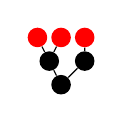
\begin{tikzpicture}[scale=.2]
\node[circle, scale=0.75, fill] (tid0) at (2.25,1.5){};
\node[circle, scale=0.75, fill] (tid1) at (1.5,3){};
\node[circle, scale=0.75, fill, red] (tid3) at (0.75,4.5){};
\node[circle, scale=0.75, fill, red] (tid4) at (2.25,4.5){};
\draw[](tid1) -- (tid3);
\draw[](tid1) -- (tid4);
\node[circle, scale=0.75, fill] (tid2) at (3.75,3){};
\node[circle, scale=0.75, fill, red] (tid5) at (3.75,4.5){};
\draw[](tid2) -- (tid5);
\draw[](tid0) -- (tid1);
\draw[](tid0) -- (tid2);
\end{tikzpicture}
\nodepart{three}
\footnotesize{4.05556}
\nodepart{four}
\footnotesize{$67\:33$}
};
 & 
\\
};
\end{scope}
\begin{scope}[yshift=\leveltopIII cm]
\matrix (line3)[column sep=0.5cm] {
\node[draw=black, rectangle split,  rectangle split parts=4] (sn0x8969bb0){
\footnotesize{66.6667}
\nodepart{two}
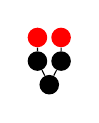
\begin{tikzpicture}[scale=.2]
\node[circle, scale=0.75, fill] (tid0) at (1.5,1.5){};
\node[circle, scale=0.75, fill] (tid1) at (0.75,3){};
\node[circle, scale=0.75, fill, red] (tid3) at (0.75,4.5){};
\draw[](tid1) -- (tid3);
\node[circle, scale=0.75, fill] (tid2) at (2.25,3){};
\node[circle, scale=0.75, fill, red] (tid4) at (2.25,4.5){};
\draw[](tid2) -- (tid4);
\draw[](tid0) -- (tid1);
\draw[](tid0) -- (tid2);
\end{tikzpicture}
\nodepart{three}
\footnotesize{3.75}
\nodepart{four}
\footnotesize{$1$}
};
 & 
\node[draw=black, rectangle split,  rectangle split parts=4] (sn0x896a3b8){
\footnotesize{33.3333}
\nodepart{two}

\begin{tikzpicture}[scale=.2]
\node[circle, scale=0.75, fill] (tid0) at (2.25,1.5){};
\node[circle, scale=0.75, fill] (tid1) at (1.5,3){};
\node[circle, scale=0.75, fill, red] (tid3) at (0.75,4.5){};
\node[circle, scale=0.75, fill, red] (tid4) at (2.25,4.5){};
\draw[](tid1) -- (tid3);
\draw[](tid1) -- (tid4);
\node[circle, scale=0.75, fill, red] (tid2) at (3.75,3){};
\draw[](tid0) -- (tid1);
\draw[](tid0) -- (tid2);
\end{tikzpicture}
\nodepart{three}
\footnotesize{3.66667}
\nodepart{four}
\footnotesize{$67\:33$}
};
 & 
\\
};
\end{scope}
\draw (sn0x8968ef8.south) -- (sn0x8969f98.north);
\draw (sn0x8969f98.south) -- (sn0x8969bb0.north);
\draw (sn0x8969f98.south) -- (sn0x896a3b8.north);
\end{tikzpicture}
\renewcommand{\leveltopI}{-15cm + \leveltop}
\renewcommand{\leveltopII}{-15cm + \leveltopI}
\renewcommand{\leveltopIII}{-15cm + \leveltopII}
\renewcommand{\leveltopIIII}{-15cm + \leveltopIII}
\renewcommand{\leveltopIIIII}{-15cm + \leveltopIIII}
\renewcommand{\leveltopIIIIII}{-15cm + \leveltopIIIII}
\renewcommand{\leveltopIIIIIII}{-15cm + \leveltopIIIIII}
\begin{tikzpicture}[scale=.2, anchor=south]
\begin{scope}[yshift=\leveltopI cm]
\matrix (line1)[column sep=0.5cm] {
\node[draw=black, rectangle split,  rectangle split parts=4] (sn0x8969e68){
\footnotesize{100}
\nodepart{two}
\begin{tikzpicture}[scale=.2]
\node[circle, scale=0.75, fill] (tid0) at (3,1.5){};
\node[circle, scale=0.75, fill] (tid1) at (2.25,3){};
\node[circle, scale=0.75, fill, red] (tid3) at (0.75,4.5){};
\node[circle, scale=0.75, fill, red] (tid4) at (2.25,4.5){};
\node[circle, scale=0.75, fill] (tid5) at (3.75,4.5){};
\draw[](tid1) -- (tid3);
\draw[](tid1) -- (tid4);
\draw[](tid1) -- (tid5);
\node[circle, scale=0.75, fill] (tid2) at (5.25,3){};
\node[circle, scale=0.75, fill, red] (tid6) at (5.25,4.5){};
\draw[](tid2) -- (tid6);
\draw[](tid0) -- (tid1);
\draw[](tid0) -- (tid2);
\end{tikzpicture}
\nodepart{three}
\footnotesize{4.37037}
\nodepart{four}
\footnotesize{$67\:33$}
};
 & 
\\
};
\end{scope}
\begin{scope}[yshift=\leveltopII cm]
\matrix (line2)[column sep=0.5cm] {
\node[draw=black, rectangle split,  rectangle split parts=4] (sn0x8969f98){
\footnotesize{66.6667}
\nodepart{two}
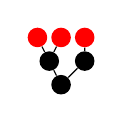
\begin{tikzpicture}[scale=.2]
\node[circle, scale=0.75, fill] (tid0) at (2.25,1.5){};
\node[circle, scale=0.75, fill] (tid1) at (1.5,3){};
\node[circle, scale=0.75, fill, red] (tid3) at (0.75,4.5){};
\node[circle, scale=0.75, fill, red] (tid4) at (2.25,4.5){};
\draw[](tid1) -- (tid3);
\draw[](tid1) -- (tid4);
\node[circle, scale=0.75, fill] (tid2) at (3.75,3){};
\node[circle, scale=0.75, fill, red] (tid5) at (3.75,4.5){};
\draw[](tid2) -- (tid5);
\draw[](tid0) -- (tid1);
\draw[](tid0) -- (tid2);
\end{tikzpicture}
\nodepart{three}
\footnotesize{4.05556}
\nodepart{four}
\footnotesize{$67\:33$}
};
 & 
\node[draw=black, rectangle split,  rectangle split parts=4] (sn0x896a940){
\footnotesize{33.3333}
\nodepart{two}
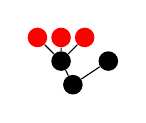
\begin{tikzpicture}[scale=.2]
\node[circle, scale=0.75, fill] (tid0) at (3,1.5){};
\node[circle, scale=0.75, fill] (tid1) at (2.25,3){};
\node[circle, scale=0.75, fill, red] (tid3) at (0.75,4.5){};
\node[circle, scale=0.75, fill, red] (tid4) at (2.25,4.5){};
\node[circle, scale=0.75, fill, red] (tid5) at (3.75,4.5){};
\draw[](tid1) -- (tid3);
\draw[](tid1) -- (tid4);
\draw[](tid1) -- (tid5);
\node[circle, scale=0.75, fill] (tid2) at (5.25,3){};
\draw[](tid0) -- (tid1);
\draw[](tid0) -- (tid2);
\end{tikzpicture}
\nodepart{three}
\footnotesize{4}
\nodepart{four}
\footnotesize{$1$}
};
 & 
\\
};
\end{scope}
\begin{scope}[yshift=\leveltopIII cm]
\matrix (line3)[column sep=0.5cm] {
\node[draw=black, rectangle split,  rectangle split parts=4] (sn0x8969bb0){
\footnotesize{44.4444}
\nodepart{two}
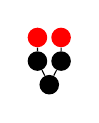
\begin{tikzpicture}[scale=.2]
\node[circle, scale=0.75, fill] (tid0) at (1.5,1.5){};
\node[circle, scale=0.75, fill] (tid1) at (0.75,3){};
\node[circle, scale=0.75, fill, red] (tid3) at (0.75,4.5){};
\draw[](tid1) -- (tid3);
\node[circle, scale=0.75, fill] (tid2) at (2.25,3){};
\node[circle, scale=0.75, fill, red] (tid4) at (2.25,4.5){};
\draw[](tid2) -- (tid4);
\draw[](tid0) -- (tid1);
\draw[](tid0) -- (tid2);
\end{tikzpicture}
\nodepart{three}
\footnotesize{3.75}
\nodepart{four}
\footnotesize{$1$}
};
 & 
\node[draw=black, rectangle split,  rectangle split parts=4] (sn0x896a3b8){
\footnotesize{55.5556}
\nodepart{two}

\begin{tikzpicture}[scale=.2]
\node[circle, scale=0.75, fill] (tid0) at (2.25,1.5){};
\node[circle, scale=0.75, fill] (tid1) at (1.5,3){};
\node[circle, scale=0.75, fill, red] (tid3) at (0.75,4.5){};
\node[circle, scale=0.75, fill, red] (tid4) at (2.25,4.5){};
\draw[](tid1) -- (tid3);
\draw[](tid1) -- (tid4);
\node[circle, scale=0.75, fill, red] (tid2) at (3.75,3){};
\draw[](tid0) -- (tid1);
\draw[](tid0) -- (tid2);
\end{tikzpicture}
\nodepart{three}
\footnotesize{3.66667}
\nodepart{four}
\footnotesize{$67\:33$}
};
 & 
\\
};
\end{scope}
\draw (sn0x8969e68.south) -- (sn0x8969f98.north);
\draw (sn0x8969e68.south) -- (sn0x896a940.north);
\draw (sn0x8969f98.south) -- (sn0x8969bb0.north);
\draw (sn0x8969f98.south) -- (sn0x896a3b8.north);
\draw (sn0x896a940.south) -- (sn0x896a3b8.north);
\end{tikzpicture}
%%% Local Variables:
%%% TeX-master: "thesis/thesis.tex"
%%% End: 
  \caption{HLF on 001112. Different runs of HLF do not necessarily produce the same result.}
  \label{fig:hlf-001112}
\end{figure}

\begin{figure}[ht]
  \centering
  \renewcommand{\leveltopI}{-15cm + \leveltop}
\renewcommand{\leveltopII}{-15cm + \leveltopI}
\renewcommand{\leveltopIII}{-15cm + \leveltopII}
\renewcommand{\leveltopIIII}{-15cm + \leveltopIII}
\renewcommand{\leveltopIIIII}{-15cm + \leveltopIIII}
\renewcommand{\leveltopIIIIII}{-15cm + \leveltopIIIII}
\renewcommand{\leveltopIIIIIII}{-15cm + \leveltopIIIIII}
\renewcommand{\leveltopIIIIIIII}{-15cm + \leveltopIIIIIII}
\renewcommand{\leveltopIIIIIIIII}{-15cm + \leveltopIIIIIIII}
\renewcommand{\leveltopIIIIIIIIII}{-15cm + \leveltopIIIIIIIII}
\renewcommand{\leveltopIIIIIIIIIII}{-15cm + \leveltopIIIIIIIIII}
\begin{tikzpicture}[scale=.2, anchor=south]
\begin{scope}[yshift=\leveltopI cm]
\matrix (line1) [column sep=1cm] {
\node[draw=black, rectangle split,  rectangle split parts=3] (sn0x14639f0){
\begin{tikzpicture}[scale=.2]
\node[circle, scale=0.75, fill] (tid0) at (3,1.5){};
\node[circle, scale=0.75, fill] (tid1) at (2.25,3){};
\node[circle, scale=0.75, fill] (tid3) at (2.25,4.5){};
\node[circle, scale=0.75, fill] (tid5) at (2.25,6){};
\node[circle, scale=0.75, fill] (tid7) at (1.5,7.5){};
\node[circle, scale=0.75, fill, red] (tid9) at (0.75,9){};
\node[circle, scale=0.75, fill, red] (tid10) at (2.25,9){};
\draw[](tid7) -- (tid9);
\draw[](tid7) -- (tid10);
\node[circle, scale=0.75, fill, red] (tid8) at (3.75,7.5){};
\draw[](tid5) -- (tid7);
\draw[](tid5) -- (tid8);
\draw[](tid3) -- (tid5);
\draw[](tid1) -- (tid3);
\node[circle, scale=0.75, fill] (tid2) at (5.25,3){};
\node[circle, scale=0.75, fill] (tid4) at (5.25,4.5){};
\node[circle, scale=0.75, fill] (tid6) at (5.25,6){};
\draw[](tid4) -- (tid6);
\draw[](tid2) -- (tid4);
\draw[](tid0) -- (tid1);
\draw[](tid0) -- (tid2);
\end{tikzpicture}
\nodepart{two}
\footnotesize{6.96798}
\nodepart{three}
\footnotesize{$33\:67$}
};
 & 
\\
};
\end{scope}
\begin{scope}[yshift=\leveltopII cm]
\matrix (line2) [column sep=1cm] {
\node[draw=black, rectangle split,  rectangle split parts=3] (sn0x1460d30){
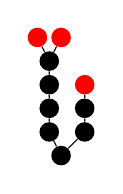
\begin{tikzpicture}[scale=.2]
\node[circle, scale=0.75, fill] (tid0) at (2.25,1.5){};
\node[circle, scale=0.75, fill] (tid1) at (1.5,3){};
\node[circle, scale=0.75, fill] (tid3) at (1.5,4.5){};
\node[circle, scale=0.75, fill] (tid5) at (1.5,6){};
\node[circle, scale=0.75, fill] (tid7) at (1.5,7.5){};
\node[circle, scale=0.75, fill, red] (tid8) at (0.75,9){};
\node[circle, scale=0.75, fill, red] (tid9) at (2.25,9){};
\draw[](tid7) -- (tid8);
\draw[](tid7) -- (tid9);
\draw[](tid5) -- (tid7);
\draw[](tid3) -- (tid5);
\draw[](tid1) -- (tid3);
\node[circle, scale=0.75, fill] (tid2) at (3.75,3){};
\node[circle, scale=0.75, fill] (tid4) at (3.75,4.5){};
\node[circle, scale=0.75, fill, red] (tid6) at (3.75,6){};
\draw[](tid4) -- (tid6);
\draw[](tid2) -- (tid4);
\draw[](tid0) -- (tid1);
\draw[](tid0) -- (tid2);
\end{tikzpicture}
\nodepart{two}
\footnotesize{6.77836}
\nodepart{three}
\footnotesize{$33\:67$}
};
 & 
\node[draw=black, rectangle split,  rectangle split parts=3] (sn0x14633d0){
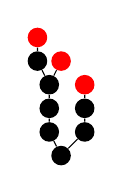
\begin{tikzpicture}[scale=.2]
\node[circle, scale=0.75, fill] (tid0) at (2.25,1.5){};
\node[circle, scale=0.75, fill] (tid1) at (1.5,3){};
\node[circle, scale=0.75, fill] (tid3) at (1.5,4.5){};
\node[circle, scale=0.75, fill] (tid5) at (1.5,6){};
\node[circle, scale=0.75, fill] (tid7) at (0.75,7.5){};
\node[circle, scale=0.75, fill, red] (tid9) at (0.75,9){};
\draw[](tid7) -- (tid9);
\node[circle, scale=0.75, fill, red] (tid8) at (2.25,7.5){};
\draw[](tid5) -- (tid7);
\draw[](tid5) -- (tid8);
\draw[](tid3) -- (tid5);
\draw[](tid1) -- (tid3);
\node[circle, scale=0.75, fill] (tid2) at (3.75,3){};
\node[circle, scale=0.75, fill] (tid4) at (3.75,4.5){};
\node[circle, scale=0.75, fill, red] (tid6) at (3.75,6){};
\draw[](tid4) -- (tid6);
\draw[](tid2) -- (tid4);
\draw[](tid0) -- (tid1);
\draw[](tid0) -- (tid2);
\end{tikzpicture}
\nodepart{two}
\footnotesize{6.56279}
\nodepart{three}
\footnotesize{$33\:33\:33$}
};
 & 
\\
};
\end{scope}
\begin{scope}[yshift=\leveltopIII cm]
\matrix (line3) [column sep=1cm] {
\node[draw=black, rectangle split,  rectangle split parts=3] (sn0x145fad0){
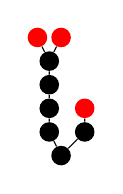
\begin{tikzpicture}[scale=.2]
\node[circle, scale=0.75, fill] (tid0) at (2.25,1.5){};
\node[circle, scale=0.75, fill] (tid1) at (1.5,3){};
\node[circle, scale=0.75, fill] (tid3) at (1.5,4.5){};
\node[circle, scale=0.75, fill] (tid5) at (1.5,6){};
\node[circle, scale=0.75, fill] (tid6) at (1.5,7.5){};
\node[circle, scale=0.75, fill, red] (tid7) at (0.75,9){};
\node[circle, scale=0.75, fill, red] (tid8) at (2.25,9){};
\draw[](tid6) -- (tid7);
\draw[](tid6) -- (tid8);
\draw[](tid5) -- (tid6);
\draw[](tid3) -- (tid5);
\draw[](tid1) -- (tid3);
\node[circle, scale=0.75, fill] (tid2) at (3.75,3){};
\node[circle, scale=0.75, fill, red] (tid4) at (3.75,4.5){};
\draw[](tid2) -- (tid4);
\draw[](tid0) -- (tid1);
\draw[](tid0) -- (tid2);
\end{tikzpicture}
\nodepart{two}
\footnotesize{6.60069}
\nodepart{three}
\footnotesize{$33\:67$}
};
 & 
\node[draw=black, rectangle split,  rectangle split parts=3] (sn0x1460050){
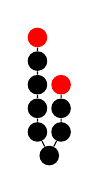
\begin{tikzpicture}[scale=.2]
\node[circle, scale=0.75, fill] (tid0) at (1.5,1.5){};
\node[circle, scale=0.75, fill] (tid1) at (0.75,3){};
\node[circle, scale=0.75, fill] (tid3) at (0.75,4.5){};
\node[circle, scale=0.75, fill] (tid5) at (0.75,6){};
\node[circle, scale=0.75, fill] (tid7) at (0.75,7.5){};
\node[circle, scale=0.75, fill, red] (tid8) at (0.75,9){};
\draw[](tid7) -- (tid8);
\draw[](tid5) -- (tid7);
\draw[](tid3) -- (tid5);
\draw[](tid1) -- (tid3);
\node[circle, scale=0.75, fill] (tid2) at (2.25,3){};
\node[circle, scale=0.75, fill] (tid4) at (2.25,4.5){};
\node[circle, scale=0.75, fill, red] (tid6) at (2.25,6){};
\draw[](tid4) -- (tid6);
\draw[](tid2) -- (tid4);
\draw[](tid0) -- (tid1);
\draw[](tid0) -- (tid2);
\end{tikzpicture}
\nodepart{two}
\footnotesize{6.36719}
\nodepart{three}
\footnotesize{$50\:50$}
};
 & 
\node[draw=black, rectangle split,  rectangle split parts=3] (sn0x1462fe0){
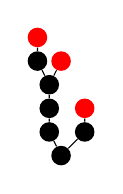
\begin{tikzpicture}[scale=.2]
\node[circle, scale=0.75, fill] (tid0) at (2.25,1.5){};
\node[circle, scale=0.75, fill] (tid1) at (1.5,3){};
\node[circle, scale=0.75, fill] (tid3) at (1.5,4.5){};
\node[circle, scale=0.75, fill] (tid5) at (1.5,6){};
\node[circle, scale=0.75, fill] (tid6) at (0.75,7.5){};
\node[circle, scale=0.75, fill, red] (tid8) at (0.75,9){};
\draw[](tid6) -- (tid8);
\node[circle, scale=0.75, fill, red] (tid7) at (2.25,7.5){};
\draw[](tid5) -- (tid6);
\draw[](tid5) -- (tid7);
\draw[](tid3) -- (tid5);
\draw[](tid1) -- (tid3);
\node[circle, scale=0.75, fill] (tid2) at (3.75,3){};
\node[circle, scale=0.75, fill, red] (tid4) at (3.75,4.5){};
\draw[](tid2) -- (tid4);
\draw[](tid0) -- (tid1);
\draw[](tid0) -- (tid2);
\end{tikzpicture}
\nodepart{two}
\footnotesize{6.36516}
\nodepart{three}
\footnotesize{$33\:33\:33$}
};
 & 
\node[draw=black, rectangle split,  rectangle split parts=3] (sn0x1462bf0){
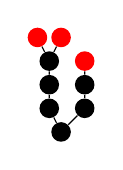
\begin{tikzpicture}[scale=.2]
\node[circle, scale=0.75, fill] (tid0) at (2.25,1.5){};
\node[circle, scale=0.75, fill] (tid1) at (1.5,3){};
\node[circle, scale=0.75, fill] (tid3) at (1.5,4.5){};
\node[circle, scale=0.75, fill] (tid5) at (1.5,6){};
\node[circle, scale=0.75, fill, red] (tid7) at (0.75,7.5){};
\node[circle, scale=0.75, fill, red] (tid8) at (2.25,7.5){};
\draw[](tid5) -- (tid7);
\draw[](tid5) -- (tid8);
\draw[](tid3) -- (tid5);
\draw[](tid1) -- (tid3);
\node[circle, scale=0.75, fill] (tid2) at (3.75,3){};
\node[circle, scale=0.75, fill] (tid4) at (3.75,4.5){};
\node[circle, scale=0.75, fill, red] (tid6) at (3.75,6){};
\draw[](tid4) -- (tid6);
\draw[](tid2) -- (tid4);
\draw[](tid0) -- (tid1);
\draw[](tid0) -- (tid2);
\end{tikzpicture}
\nodepart{two}
\footnotesize{5.95602}
\nodepart{three}
\footnotesize{$67\:33$}
};
 & 
\\
};
\end{scope}
\begin{scope}[yshift=\leveltopIIII cm]
\matrix (line4) [column sep=1cm] {
\node[draw=black, rectangle split,  rectangle split parts=3] (sn0x145e900){
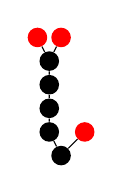
\begin{tikzpicture}[scale=.2]
\node[circle, scale=0.75, fill] (tid0) at (2.25,1.5){};
\node[circle, scale=0.75, fill] (tid1) at (1.5,3){};
\node[circle, scale=0.75, fill] (tid3) at (1.5,4.5){};
\node[circle, scale=0.75, fill] (tid4) at (1.5,6){};
\node[circle, scale=0.75, fill] (tid5) at (1.5,7.5){};
\node[circle, scale=0.75, fill, red] (tid6) at (0.75,9){};
\node[circle, scale=0.75, fill, red] (tid7) at (2.25,9){};
\draw[](tid5) -- (tid6);
\draw[](tid5) -- (tid7);
\draw[](tid4) -- (tid5);
\draw[](tid3) -- (tid4);
\draw[](tid1) -- (tid3);
\node[circle, scale=0.75, fill, red] (tid2) at (3.75,3){};
\draw[](tid0) -- (tid1);
\draw[](tid0) -- (tid2);
\end{tikzpicture}
\nodepart{two}
\footnotesize{6.52083}
\nodepart{three}
\footnotesize{$33\:67$}
};
 & 
\node[draw=black, rectangle split,  rectangle split parts=3] (sn0x145fa00){
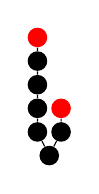
\begin{tikzpicture}[scale=.2]
\node[circle, scale=0.75, fill] (tid0) at (1.5,1.5){};
\node[circle, scale=0.75, fill] (tid1) at (0.75,3){};
\node[circle, scale=0.75, fill] (tid3) at (0.75,4.5){};
\node[circle, scale=0.75, fill] (tid5) at (0.75,6){};
\node[circle, scale=0.75, fill] (tid6) at (0.75,7.5){};
\node[circle, scale=0.75, fill, red] (tid7) at (0.75,9){};
\draw[](tid6) -- (tid7);
\draw[](tid5) -- (tid6);
\draw[](tid3) -- (tid5);
\draw[](tid1) -- (tid3);
\node[circle, scale=0.75, fill] (tid2) at (2.25,3){};
\node[circle, scale=0.75, fill, red] (tid4) at (2.25,4.5){};
\draw[](tid2) -- (tid4);
\draw[](tid0) -- (tid1);
\draw[](tid0) -- (tid2);
\end{tikzpicture}
\nodepart{two}
\footnotesize{6.14062}
\nodepart{three}
\footnotesize{$50\:50$}
};
 & 
\node[draw=black, rectangle split,  rectangle split parts=3] (sn0x145ff80){
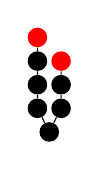
\begin{tikzpicture}[scale=.2]
\node[circle, scale=0.75, fill] (tid0) at (1.5,1.5){};
\node[circle, scale=0.75, fill] (tid1) at (0.75,3){};
\node[circle, scale=0.75, fill] (tid3) at (0.75,4.5){};
\node[circle, scale=0.75, fill] (tid5) at (0.75,6){};
\node[circle, scale=0.75, fill, red] (tid7) at (0.75,7.5){};
\draw[](tid5) -- (tid7);
\draw[](tid3) -- (tid5);
\draw[](tid1) -- (tid3);
\node[circle, scale=0.75, fill] (tid2) at (2.25,3){};
\node[circle, scale=0.75, fill] (tid4) at (2.25,4.5){};
\node[circle, scale=0.75, fill, red] (tid6) at (2.25,6){};
\draw[](tid4) -- (tid6);
\draw[](tid2) -- (tid4);
\draw[](tid0) -- (tid1);
\draw[](tid0) -- (tid2);
\end{tikzpicture}
\nodepart{two}
\footnotesize{5.59375}
\nodepart{three}
\footnotesize{$50\:50$}
};
 & 
\node[draw=black, rectangle split,  rectangle split parts=3] (sn0x1462420){
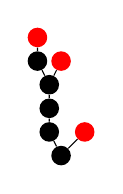
\begin{tikzpicture}[scale=.2]
\node[circle, scale=0.75, fill] (tid0) at (2.25,1.5){};
\node[circle, scale=0.75, fill] (tid1) at (1.5,3){};
\node[circle, scale=0.75, fill] (tid3) at (1.5,4.5){};
\node[circle, scale=0.75, fill] (tid4) at (1.5,6){};
\node[circle, scale=0.75, fill] (tid5) at (0.75,7.5){};
\node[circle, scale=0.75, fill, red] (tid7) at (0.75,9){};
\draw[](tid5) -- (tid7);
\node[circle, scale=0.75, fill, red] (tid6) at (2.25,7.5){};
\draw[](tid4) -- (tid5);
\draw[](tid4) -- (tid6);
\draw[](tid3) -- (tid4);
\draw[](tid1) -- (tid3);
\node[circle, scale=0.75, fill, red] (tid2) at (3.75,3){};
\draw[](tid0) -- (tid1);
\draw[](tid0) -- (tid2);
\end{tikzpicture}
\nodepart{two}
\footnotesize{6.27431}
\nodepart{three}
\footnotesize{$33\:33\:33$}
};
 & 
\node[draw=black, rectangle split,  rectangle split parts=3] (sn0x14624f0){
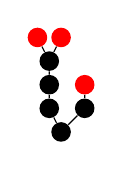
\begin{tikzpicture}[scale=.2]
\node[circle, scale=0.75, fill] (tid0) at (2.25,1.5){};
\node[circle, scale=0.75, fill] (tid1) at (1.5,3){};
\node[circle, scale=0.75, fill] (tid3) at (1.5,4.5){};
\node[circle, scale=0.75, fill] (tid5) at (1.5,6){};
\node[circle, scale=0.75, fill, red] (tid6) at (0.75,7.5){};
\node[circle, scale=0.75, fill, red] (tid7) at (2.25,7.5){};
\draw[](tid5) -- (tid6);
\draw[](tid5) -- (tid7);
\draw[](tid3) -- (tid5);
\draw[](tid1) -- (tid3);
\node[circle, scale=0.75, fill] (tid2) at (3.75,3){};
\node[circle, scale=0.75, fill, red] (tid4) at (3.75,4.5){};
\draw[](tid2) -- (tid4);
\draw[](tid0) -- (tid1);
\draw[](tid0) -- (tid2);
\end{tikzpicture}
\nodepart{two}
\footnotesize{5.68056}
\nodepart{three}
\footnotesize{$67\:33$}
};
 & 
\\
};
\end{scope}
\begin{scope}[yshift=\leveltopIIIII cm]
\matrix (line5) [column sep=1cm] {
\node[draw=black, rectangle split,  rectangle split parts=3] (sn0x145d480){
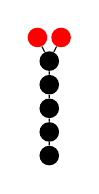
\begin{tikzpicture}[scale=.2]
\node[circle, scale=0.75, fill] (tid0) at (1.5,1.5){};
\node[circle, scale=0.75, fill] (tid1) at (1.5,3){};
\node[circle, scale=0.75, fill] (tid2) at (1.5,4.5){};
\node[circle, scale=0.75, fill] (tid3) at (1.5,6){};
\node[circle, scale=0.75, fill] (tid4) at (1.5,7.5){};
\node[circle, scale=0.75, fill, red] (tid5) at (0.75,9){};
\node[circle, scale=0.75, fill, red] (tid6) at (2.25,9){};
\draw[](tid4) -- (tid5);
\draw[](tid4) -- (tid6);
\draw[](tid3) -- (tid4);
\draw[](tid2) -- (tid3);
\draw[](tid1) -- (tid2);
\draw[](tid0) -- (tid1);
\end{tikzpicture}
\nodepart{two}
\footnotesize{6.5}
\nodepart{three}
\footnotesize{$1$}
};
 & 
\node[draw=black, rectangle split,  rectangle split parts=3] (sn0x145e670){
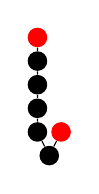
\begin{tikzpicture}[scale=.2]
\node[circle, scale=0.75, fill] (tid0) at (1.5,1.5){};
\node[circle, scale=0.75, fill] (tid1) at (0.75,3){};
\node[circle, scale=0.75, fill] (tid3) at (0.75,4.5){};
\node[circle, scale=0.75, fill] (tid4) at (0.75,6){};
\node[circle, scale=0.75, fill] (tid5) at (0.75,7.5){};
\node[circle, scale=0.75, fill, red] (tid6) at (0.75,9){};
\draw[](tid5) -- (tid6);
\draw[](tid4) -- (tid5);
\draw[](tid3) -- (tid4);
\draw[](tid1) -- (tid3);
\node[circle, scale=0.75, fill, red] (tid2) at (2.25,3){};
\draw[](tid0) -- (tid1);
\draw[](tid0) -- (tid2);
\end{tikzpicture}
\nodepart{two}
\footnotesize{6.03125}
\nodepart{three}
\footnotesize{$50\:50$}
};
 & 
\node[draw=black, rectangle split,  rectangle split parts=3] (sn0x145f770){
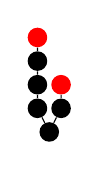
\begin{tikzpicture}[scale=.2]
\node[circle, scale=0.75, fill] (tid0) at (1.5,1.5){};
\node[circle, scale=0.75, fill] (tid1) at (0.75,3){};
\node[circle, scale=0.75, fill] (tid3) at (0.75,4.5){};
\node[circle, scale=0.75, fill] (tid5) at (0.75,6){};
\node[circle, scale=0.75, fill, red] (tid6) at (0.75,7.5){};
\draw[](tid5) -- (tid6);
\draw[](tid3) -- (tid5);
\draw[](tid1) -- (tid3);
\node[circle, scale=0.75, fill] (tid2) at (2.25,3){};
\node[circle, scale=0.75, fill, red] (tid4) at (2.25,4.5){};
\draw[](tid2) -- (tid4);
\draw[](tid0) -- (tid1);
\draw[](tid0) -- (tid2);
\end{tikzpicture}
\nodepart{two}
\footnotesize{5.25}
\nodepart{three}
\footnotesize{$50\:50$}
};
 & 
\node[draw=black, rectangle split,  rectangle split parts=3] (sn0x1460b00){
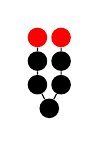
\begin{tikzpicture}[scale=.2]
\node[circle, scale=0.75, fill] (tid0) at (1.5,1.5){};
\node[circle, scale=0.75, fill] (tid1) at (0.75,3){};
\node[circle, scale=0.75, fill] (tid3) at (0.75,4.5){};
\node[circle, scale=0.75, fill, red] (tid5) at (0.75,6){};
\draw[](tid3) -- (tid5);
\draw[](tid1) -- (tid3);
\node[circle, scale=0.75, fill] (tid2) at (2.25,3){};
\node[circle, scale=0.75, fill] (tid4) at (2.25,4.5){};
\node[circle, scale=0.75, fill, red] (tid6) at (2.25,6){};
\draw[](tid4) -- (tid6);
\draw[](tid2) -- (tid4);
\draw[](tid0) -- (tid1);
\draw[](tid0) -- (tid2);
\end{tikzpicture}
\nodepart{two}
\footnotesize{4.9375}
\nodepart{three}
\footnotesize{$1$}
};
 & 
\node[draw=black, rectangle split,  rectangle split parts=3] (sn0x1462350){
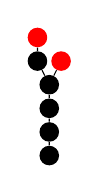
\begin{tikzpicture}[scale=.2]
\node[circle, scale=0.75, fill] (tid0) at (1.5,1.5){};
\node[circle, scale=0.75, fill] (tid1) at (1.5,3){};
\node[circle, scale=0.75, fill] (tid2) at (1.5,4.5){};
\node[circle, scale=0.75, fill] (tid3) at (1.5,6){};
\node[circle, scale=0.75, fill] (tid4) at (0.75,7.5){};
\node[circle, scale=0.75, fill, red] (tid6) at (0.75,9){};
\draw[](tid4) -- (tid6);
\node[circle, scale=0.75, fill, red] (tid5) at (2.25,7.5){};
\draw[](tid3) -- (tid4);
\draw[](tid3) -- (tid5);
\draw[](tid2) -- (tid3);
\draw[](tid1) -- (tid2);
\draw[](tid0) -- (tid1);
\end{tikzpicture}
\nodepart{two}
\footnotesize{6.25}
\nodepart{three}
\footnotesize{$50\:50$}
};
 & 
\node[draw=black, rectangle split,  rectangle split parts=3] (sn0x14628e0){
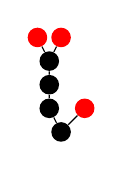
\begin{tikzpicture}[scale=.2]
\node[circle, scale=0.75, fill] (tid0) at (2.25,1.5){};
\node[circle, scale=0.75, fill] (tid1) at (1.5,3){};
\node[circle, scale=0.75, fill] (tid3) at (1.5,4.5){};
\node[circle, scale=0.75, fill] (tid4) at (1.5,6){};
\node[circle, scale=0.75, fill, red] (tid5) at (0.75,7.5){};
\node[circle, scale=0.75, fill, red] (tid6) at (2.25,7.5){};
\draw[](tid4) -- (tid5);
\draw[](tid4) -- (tid6);
\draw[](tid3) -- (tid4);
\draw[](tid1) -- (tid3);
\node[circle, scale=0.75, fill, red] (tid2) at (3.75,3){};
\draw[](tid0) -- (tid1);
\draw[](tid0) -- (tid2);
\end{tikzpicture}
\nodepart{two}
\footnotesize{5.54167}
\nodepart{three}
\footnotesize{$67\:33$}
};
 & 
\\
};
\end{scope}
\begin{scope}[yshift=\leveltopIIIIII cm]
\matrix (line6) [column sep=1cm] {
\node[draw=black, rectangle split,  rectangle split parts=3] (sn0x145d0f0){
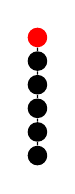
\begin{tikzpicture}[scale=.2]
\node[circle, scale=0.75, fill] (tid0) at (0.75,1.5){};
\node[circle, scale=0.75, fill] (tid1) at (0.75,3){};
\node[circle, scale=0.75, fill] (tid2) at (0.75,4.5){};
\node[circle, scale=0.75, fill] (tid3) at (0.75,6){};
\node[circle, scale=0.75, fill] (tid4) at (0.75,7.5){};
\node[circle, scale=0.75, fill, red] (tid5) at (0.75,9){};
\draw[](tid4) -- (tid5);
\draw[](tid3) -- (tid4);
\draw[](tid2) -- (tid3);
\draw[](tid1) -- (tid2);
\draw[](tid0) -- (tid1);
\end{tikzpicture}
\nodepart{two}
\footnotesize{6}
\nodepart{three}
\footnotesize{$1$}
};
 & 
\node[draw=black, rectangle split,  rectangle split parts=3] (sn0x145e380){
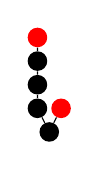
\begin{tikzpicture}[scale=.2]
\node[circle, scale=0.75, fill] (tid0) at (1.5,1.5){};
\node[circle, scale=0.75, fill] (tid1) at (0.75,3){};
\node[circle, scale=0.75, fill] (tid3) at (0.75,4.5){};
\node[circle, scale=0.75, fill] (tid4) at (0.75,6){};
\node[circle, scale=0.75, fill, red] (tid5) at (0.75,7.5){};
\draw[](tid4) -- (tid5);
\draw[](tid3) -- (tid4);
\draw[](tid1) -- (tid3);
\node[circle, scale=0.75, fill, red] (tid2) at (2.25,3){};
\draw[](tid0) -- (tid1);
\draw[](tid0) -- (tid2);
\end{tikzpicture}
\nodepart{two}
\footnotesize{5.0625}
\nodepart{three}
\footnotesize{$50\:50$}
};
 & 
\node[draw=black, rectangle split,  rectangle split parts=3] (sn0x145ec40){
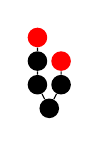
\begin{tikzpicture}[scale=.2]
\node[circle, scale=0.75, fill] (tid0) at (1.5,1.5){};
\node[circle, scale=0.75, fill] (tid1) at (0.75,3){};
\node[circle, scale=0.75, fill] (tid3) at (0.75,4.5){};
\node[circle, scale=0.75, fill, red] (tid5) at (0.75,6){};
\draw[](tid3) -- (tid5);
\draw[](tid1) -- (tid3);
\node[circle, scale=0.75, fill] (tid2) at (2.25,3){};
\node[circle, scale=0.75, fill, red] (tid4) at (2.25,4.5){};
\draw[](tid2) -- (tid4);
\draw[](tid0) -- (tid1);
\draw[](tid0) -- (tid2);
\end{tikzpicture}
\nodepart{two}
\footnotesize{4.4375}
\nodepart{three}
\footnotesize{$50\:50$}
};
 & 
\node[draw=black, rectangle split,  rectangle split parts=3] (sn0x1461150){
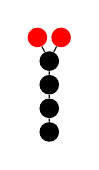
\begin{tikzpicture}[scale=.2]
\node[circle, scale=0.75, fill] (tid0) at (1.5,1.5){};
\node[circle, scale=0.75, fill] (tid1) at (1.5,3){};
\node[circle, scale=0.75, fill] (tid2) at (1.5,4.5){};
\node[circle, scale=0.75, fill] (tid3) at (1.5,6){};
\node[circle, scale=0.75, fill, red] (tid4) at (0.75,7.5){};
\node[circle, scale=0.75, fill, red] (tid5) at (2.25,7.5){};
\draw[](tid3) -- (tid4);
\draw[](tid3) -- (tid5);
\draw[](tid2) -- (tid3);
\draw[](tid1) -- (tid2);
\draw[](tid0) -- (tid1);
\end{tikzpicture}
\nodepart{two}
\footnotesize{5.5}
\nodepart{three}
\footnotesize{$1$}
};
 & 
\\
};
\end{scope}
\begin{scope}[yshift=\leveltopIIIIIII cm]
\matrix (line7) [column sep=1cm] {
\node[draw=black, rectangle split,  rectangle split parts=3] (sn0x145cdf0){
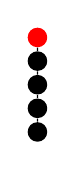
\begin{tikzpicture}[scale=.2]
\node[circle, scale=0.75, fill] (tid0) at (0.75,1.5){};
\node[circle, scale=0.75, fill] (tid1) at (0.75,3){};
\node[circle, scale=0.75, fill] (tid2) at (0.75,4.5){};
\node[circle, scale=0.75, fill] (tid3) at (0.75,6){};
\node[circle, scale=0.75, fill, red] (tid4) at (0.75,7.5){};
\draw[](tid3) -- (tid4);
\draw[](tid2) -- (tid3);
\draw[](tid1) -- (tid2);
\draw[](tid0) -- (tid1);
\end{tikzpicture}
\nodepart{two}
\footnotesize{5}
\nodepart{three}
\footnotesize{$1$}
};
 & 
\node[draw=black, rectangle split,  rectangle split parts=3] (sn0x145e0d0){
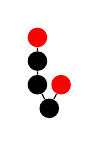
\begin{tikzpicture}[scale=.2]
\node[circle, scale=0.75, fill] (tid0) at (1.5,1.5){};
\node[circle, scale=0.75, fill] (tid1) at (0.75,3){};
\node[circle, scale=0.75, fill] (tid3) at (0.75,4.5){};
\node[circle, scale=0.75, fill, red] (tid4) at (0.75,6){};
\draw[](tid3) -- (tid4);
\draw[](tid1) -- (tid3);
\node[circle, scale=0.75, fill, red] (tid2) at (2.25,3){};
\draw[](tid0) -- (tid1);
\draw[](tid0) -- (tid2);
\end{tikzpicture}
\nodepart{two}
\footnotesize{4.125}
\nodepart{three}
\footnotesize{$50\:50$}
};
 & 
\node[draw=black, rectangle split,  rectangle split parts=3] (sn0x145eb50){
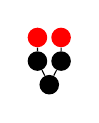
\begin{tikzpicture}[scale=.2]
\node[circle, scale=0.75, fill] (tid0) at (1.5,1.5){};
\node[circle, scale=0.75, fill] (tid1) at (0.75,3){};
\node[circle, scale=0.75, fill, red] (tid3) at (0.75,4.5){};
\draw[](tid1) -- (tid3);
\node[circle, scale=0.75, fill] (tid2) at (2.25,3){};
\node[circle, scale=0.75, fill, red] (tid4) at (2.25,4.5){};
\draw[](tid2) -- (tid4);
\draw[](tid0) -- (tid1);
\draw[](tid0) -- (tid2);
\end{tikzpicture}
\nodepart{two}
\footnotesize{3.75}
\nodepart{three}
\footnotesize{$1$}
};
 & 
\\
};
\end{scope}
\begin{scope}[yshift=\leveltopIIIIIIII cm]
\matrix (line8) [column sep=1cm] {
\node[draw=black, rectangle split,  rectangle split parts=3] (sn0x145cd20){
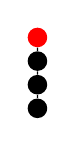
\begin{tikzpicture}[scale=.2]
\node[circle, scale=0.75, fill] (tid0) at (0.75,1.5){};
\node[circle, scale=0.75, fill] (tid1) at (0.75,3){};
\node[circle, scale=0.75, fill] (tid2) at (0.75,4.5){};
\node[circle, scale=0.75, fill, red] (tid3) at (0.75,6){};
\draw[](tid2) -- (tid3);
\draw[](tid1) -- (tid2);
\draw[](tid0) -- (tid1);
\end{tikzpicture}
\nodepart{two}
\footnotesize{4}
\nodepart{three}
\footnotesize{$1$}
};
 & 
\node[draw=black, rectangle split,  rectangle split parts=3] (sn0x145d820){
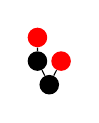
\begin{tikzpicture}[scale=.2]
\node[circle, scale=0.75, fill] (tid0) at (1.5,1.5){};
\node[circle, scale=0.75, fill] (tid1) at (0.75,3){};
\node[circle, scale=0.75, fill, red] (tid3) at (0.75,4.5){};
\draw[](tid1) -- (tid3);
\node[circle, scale=0.75, fill, red] (tid2) at (2.25,3){};
\draw[](tid0) -- (tid1);
\draw[](tid0) -- (tid2);
\end{tikzpicture}
\nodepart{two}
\footnotesize{3.25}
\nodepart{three}
\footnotesize{$50\:50$}
};
 & 
\\
};
\end{scope}
\begin{scope}[yshift=\leveltopIIIIIIIII cm]
\matrix (line9) [column sep=1cm] {
\node[draw=black, rectangle split,  rectangle split parts=3] (sn0x145b6b0){
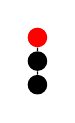
\begin{tikzpicture}[scale=.2]
\node[circle, scale=0.75, fill] (tid0) at (0.75,1.5){};
\node[circle, scale=0.75, fill] (tid1) at (0.75,3){};
\node[circle, scale=0.75, fill, red] (tid2) at (0.75,4.5){};
\draw[](tid1) -- (tid2);
\draw[](tid0) -- (tid1);
\end{tikzpicture}
\nodepart{two}
\footnotesize{3}
\nodepart{three}
\footnotesize{$1$}
};
 & 
\node[draw=black, rectangle split,  rectangle split parts=3] (sn0x145d710){

\begin{tikzpicture}[scale=.2]
\node[circle, scale=0.75, fill] (tid0) at (1.5,1.5){};
\node[circle, scale=0.75, fill, red] (tid1) at (0.75,3){};
\node[circle, scale=0.75, fill, red] (tid2) at (2.25,3){};
\draw[](tid0) -- (tid1);
\draw[](tid0) -- (tid2);
\end{tikzpicture}
\nodepart{two}
\footnotesize{2.5}
\nodepart{three}
\footnotesize{$1$}
};
 & 
\\
};
\end{scope}
\begin{scope}[yshift=\leveltopIIIIIIIIII cm]
\matrix (line10) [column sep=1cm] {
\node[draw=black, rectangle split,  rectangle split parts=3] (sn0x145aea0){

\begin{tikzpicture}[scale=.2]
\node[circle, scale=0.75, fill] (tid0) at (0.75,1.5){};
\node[circle, scale=0.75, fill, red] (tid1) at (0.75,3){};
\draw[](tid0) -- (tid1);
\end{tikzpicture}
\nodepart{two}
\footnotesize{2}
\nodepart{three}
\footnotesize{$1$}
};
 & 
\\
};
\end{scope}
\begin{scope}[yshift=\leveltopIIIIIIIIIII cm]
\matrix (line11) [column sep=1cm] {
\node[draw=black, rectangle split,  rectangle split parts=3] (sn0x145b5e0){

\begin{tikzpicture}[scale=.2]
\node[circle, scale=0.75, fill, red] (tid0) at (0.75,1.5){};
\end{tikzpicture}
\nodepart{two}
\footnotesize{1}
\nodepart{three}
\footnotesize{$$}
};
 & 
\\
};
\end{scope}
\begin{scope}[yshift=\leveltopIIIIIIIIIIII cm]
\matrix (line12) [column sep=1cm] {
\\
};
\end{scope}
\draw (sn0x14639f0.south) -- (sn0x1460d30.north);
\draw (sn0x14639f0.south) -- (sn0x14633d0.north);
\draw (sn0x1460d30.south) -- (sn0x145fad0.north);
\draw (sn0x1460d30.south) -- (sn0x1460050.north);
\draw (sn0x14633d0.south) -- (sn0x1462fe0.north);
\draw (sn0x14633d0.south) -- (sn0x1460050.north);
\draw (sn0x14633d0.south) -- (sn0x1462bf0.north);
\draw (sn0x145fad0.south) -- (sn0x145e900.north);
\draw (sn0x145fad0.south) -- (sn0x145fa00.north);
\draw (sn0x1460050.south) -- (sn0x145fa00.north);
\draw (sn0x1460050.south) -- (sn0x145ff80.north);
\draw (sn0x1462fe0.south) -- (sn0x1462420.north);
\draw (sn0x1462fe0.south) -- (sn0x145fa00.north);
\draw (sn0x1462fe0.south) -- (sn0x14624f0.north);
\draw (sn0x1462bf0.south) -- (sn0x14624f0.north);
\draw (sn0x1462bf0.south) -- (sn0x145ff80.north);
\draw (sn0x145e900.south) -- (sn0x145d480.north);
\draw (sn0x145e900.south) -- (sn0x145e670.north);
\draw (sn0x145fa00.south) -- (sn0x145e670.north);
\draw (sn0x145fa00.south) -- (sn0x145f770.north);
\draw (sn0x145ff80.south) -- (sn0x145f770.north);
\draw (sn0x145ff80.south) -- (sn0x1460b00.north);
\draw (sn0x1462420.south) -- (sn0x1462350.north);
\draw (sn0x1462420.south) -- (sn0x145e670.north);
\draw (sn0x1462420.south) -- (sn0x14628e0.north);
\draw (sn0x14624f0.south) -- (sn0x14628e0.north);
\draw (sn0x14624f0.south) -- (sn0x145f770.north);
\draw (sn0x145d480.south) -- (sn0x145d0f0.north);
\draw (sn0x145e670.south) -- (sn0x145d0f0.north);
\draw (sn0x145e670.south) -- (sn0x145e380.north);
\draw (sn0x145f770.south) -- (sn0x145e380.north);
\draw (sn0x145f770.south) -- (sn0x145ec40.north);
\draw (sn0x1460b00.south) -- (sn0x145ec40.north);
\draw (sn0x1462350.south) -- (sn0x145d0f0.north);
\draw (sn0x1462350.south) -- (sn0x1461150.north);
\draw (sn0x14628e0.south) -- (sn0x1461150.north);
\draw (sn0x14628e0.south) -- (sn0x145e380.north);
\draw (sn0x145d0f0.south) -- (sn0x145cdf0.north);
\draw (sn0x145e380.south) -- (sn0x145cdf0.north);
\draw (sn0x145e380.south) -- (sn0x145e0d0.north);
\draw (sn0x145ec40.south) -- (sn0x145e0d0.north);
\draw (sn0x145ec40.south) -- (sn0x145eb50.north);
\draw (sn0x1461150.south) -- (sn0x145cdf0.north);
\draw (sn0x145cdf0.south) -- (sn0x145cd20.north);
\draw (sn0x145e0d0.south) -- (sn0x145cd20.north);
\draw (sn0x145e0d0.south) -- (sn0x145d820.north);
\draw (sn0x145eb50.south) -- (sn0x145d820.north);
\draw (sn0x145cd20.south) -- (sn0x145b6b0.north);
\draw (sn0x145d820.south) -- (sn0x145b6b0.north);
\draw (sn0x145d820.south) -- (sn0x145d710.north);
\draw (sn0x145b6b0.south) -- (sn0x145aea0.north);
\draw (sn0x145d710.south) -- (sn0x145aea0.north);
\draw (sn0x145aea0.south) -- (sn0x145b5e0.north);
\end{tikzpicture}

%%% Local Variables:
%%% TeX-master: "thesis/thesis.tex"
%%% End: 

  \renewcommand{\leveltopI}{-15cm + \leveltop}
\renewcommand{\leveltopII}{-15cm + \leveltopI}
\renewcommand{\leveltopIII}{-15cm + \leveltopII}
\renewcommand{\leveltopIIII}{-15cm + \leveltopIII}
\renewcommand{\leveltopIIIII}{-15cm + \leveltopIIII}
\renewcommand{\leveltopIIIIII}{-15cm + \leveltopIIIII}
\renewcommand{\leveltopIIIIIII}{-15cm + \leveltopIIIIII}
\renewcommand{\leveltopIIIIIIII}{-15cm + \leveltopIIIIIII}
\renewcommand{\leveltopIIIIIIIII}{-15cm + \leveltopIIIIIIII}
\renewcommand{\leveltopIIIIIIIIII}{-15cm + \leveltopIIIIIIIII}
\renewcommand{\leveltopIIIIIIIIIII}{-15cm + \leveltopIIIIIIIIII}
\begin{tikzpicture}[scale=.2, anchor=south]
\begin{scope}[yshift=\leveltopI cm]
\matrix (line1) [column sep=1cm] {
\node[draw=black, rectangle split,  rectangle split parts=4] (sn0x18908d0){
\footnotesize{1}
\nodepart{two}
\begin{tikzpicture}[scale=.2]
\node[circle, scale=0.75, fill] (tid0) at (3,1.5){};
\node[circle, scale=0.75, fill] (tid1) at (2.25,3){};
\node[circle, scale=0.75, fill] (tid3) at (2.25,4.5){};
\node[circle, scale=0.75, fill] (tid5) at (2.25,6){};
\node[circle, scale=0.75, fill] (tid7) at (1.5,7.5){};
\node[circle, scale=0.75, fill, red] (tid9) at (0.75,9){};
\node[circle, scale=0.75, fill, red] (tid10) at (2.25,9){};
\draw[](tid7) -- (tid9);
\draw[](tid7) -- (tid10);
\node[circle, scale=0.75, fill] (tid8) at (3.75,7.5){};
\draw[](tid5) -- (tid7);
\draw[](tid5) -- (tid8);
\draw[](tid3) -- (tid5);
\draw[](tid1) -- (tid3);
\node[circle, scale=0.75, fill] (tid2) at (5.25,3){};
\node[circle, scale=0.75, fill] (tid4) at (5.25,4.5){};
\node[circle, scale=0.75, fill, red] (tid6) at (5.25,6){};
\draw[](tid4) -- (tid6);
\draw[](tid2) -- (tid4);
\draw[](tid0) -- (tid1);
\draw[](tid0) -- (tid2);
\end{tikzpicture}
\nodepart{three}
\footnotesize{6.96753}
\nodepart{four}
\footnotesize{$33\:67$}
};
 & 
\\
};
\end{scope}
\begin{scope}[yshift=\leveltopII cm]
\matrix (line2) [column sep=1cm] {
\node[draw=black, rectangle split,  rectangle split parts=4] (sn0x188ec30){
\footnotesize{0.333333}
\nodepart{two}
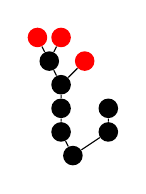
\begin{tikzpicture}[scale=.2]
\node[circle, scale=0.75, fill] (tid0) at (3,1.5){};
\node[circle, scale=0.75, fill] (tid1) at (2.25,3){};
\node[circle, scale=0.75, fill] (tid3) at (2.25,4.5){};
\node[circle, scale=0.75, fill] (tid5) at (2.25,6){};
\node[circle, scale=0.75, fill] (tid6) at (1.5,7.5){};
\node[circle, scale=0.75, fill, red] (tid8) at (0.75,9){};
\node[circle, scale=0.75, fill, red] (tid9) at (2.25,9){};
\draw[](tid6) -- (tid8);
\draw[](tid6) -- (tid9);
\node[circle, scale=0.75, fill, red] (tid7) at (3.75,7.5){};
\draw[](tid5) -- (tid6);
\draw[](tid5) -- (tid7);
\draw[](tid3) -- (tid5);
\draw[](tid1) -- (tid3);
\node[circle, scale=0.75, fill] (tid2) at (5.25,3){};
\node[circle, scale=0.75, fill] (tid4) at (5.25,4.5){};
\draw[](tid2) -- (tid4);
\draw[](tid0) -- (tid1);
\draw[](tid0) -- (tid2);
\end{tikzpicture}
\nodepart{three}
\footnotesize{6.77701}
\nodepart{four}
\footnotesize{$33\:67$}
};
 & 
\node[draw=black, rectangle split,  rectangle split parts=4] (sn0x18906a0){
\footnotesize{0.666667}
\nodepart{two}
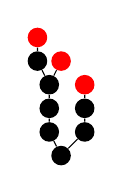
\begin{tikzpicture}[scale=.2]
\node[circle, scale=0.75, fill] (tid0) at (2.25,1.5){};
\node[circle, scale=0.75, fill] (tid1) at (1.5,3){};
\node[circle, scale=0.75, fill] (tid3) at (1.5,4.5){};
\node[circle, scale=0.75, fill] (tid5) at (1.5,6){};
\node[circle, scale=0.75, fill] (tid7) at (0.75,7.5){};
\node[circle, scale=0.75, fill, red] (tid9) at (0.75,9){};
\draw[](tid7) -- (tid9);
\node[circle, scale=0.75, fill, red] (tid8) at (2.25,7.5){};
\draw[](tid5) -- (tid7);
\draw[](tid5) -- (tid8);
\draw[](tid3) -- (tid5);
\draw[](tid1) -- (tid3);
\node[circle, scale=0.75, fill] (tid2) at (3.75,3){};
\node[circle, scale=0.75, fill] (tid4) at (3.75,4.5){};
\node[circle, scale=0.75, fill, red] (tid6) at (3.75,6){};
\draw[](tid4) -- (tid6);
\draw[](tid2) -- (tid4);
\draw[](tid0) -- (tid1);
\draw[](tid0) -- (tid2);
\end{tikzpicture}
\nodepart{three}
\footnotesize{6.56279}
\nodepart{four}
\footnotesize{$33\:33\:33$}
};
 & 
\\
};
\end{scope}
\begin{scope}[yshift=\leveltopIII cm]
\matrix (line3) [column sep=1cm] {
\node[draw=black, rectangle split,  rectangle split parts=4] (sn0x188e220){
\footnotesize{0.111111}
\nodepart{two}
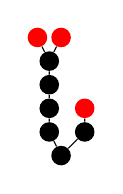
\begin{tikzpicture}[scale=.2]
\node[circle, scale=0.75, fill] (tid0) at (2.25,1.5){};
\node[circle, scale=0.75, fill] (tid1) at (1.5,3){};
\node[circle, scale=0.75, fill] (tid3) at (1.5,4.5){};
\node[circle, scale=0.75, fill] (tid5) at (1.5,6){};
\node[circle, scale=0.75, fill] (tid6) at (1.5,7.5){};
\node[circle, scale=0.75, fill, red] (tid7) at (0.75,9){};
\node[circle, scale=0.75, fill, red] (tid8) at (2.25,9){};
\draw[](tid6) -- (tid7);
\draw[](tid6) -- (tid8);
\draw[](tid5) -- (tid6);
\draw[](tid3) -- (tid5);
\draw[](tid1) -- (tid3);
\node[circle, scale=0.75, fill] (tid2) at (3.75,3){};
\node[circle, scale=0.75, fill, red] (tid4) at (3.75,4.5){};
\draw[](tid2) -- (tid4);
\draw[](tid0) -- (tid1);
\draw[](tid0) -- (tid2);
\end{tikzpicture}
\nodepart{three}
\footnotesize{6.60069}
\nodepart{four}
\footnotesize{$33\:67$}
};
 & 
\node[draw=black, rectangle split,  rectangle split parts=4] (sn0x188d8a0){
\footnotesize{0.444444}
\nodepart{two}
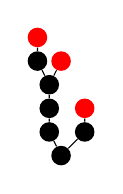
\begin{tikzpicture}[scale=.2]
\node[circle, scale=0.75, fill] (tid0) at (2.25,1.5){};
\node[circle, scale=0.75, fill] (tid1) at (1.5,3){};
\node[circle, scale=0.75, fill] (tid3) at (1.5,4.5){};
\node[circle, scale=0.75, fill] (tid5) at (1.5,6){};
\node[circle, scale=0.75, fill] (tid6) at (0.75,7.5){};
\node[circle, scale=0.75, fill, red] (tid8) at (0.75,9){};
\draw[](tid6) -- (tid8);
\node[circle, scale=0.75, fill, red] (tid7) at (2.25,7.5){};
\draw[](tid5) -- (tid6);
\draw[](tid5) -- (tid7);
\draw[](tid3) -- (tid5);
\draw[](tid1) -- (tid3);
\node[circle, scale=0.75, fill] (tid2) at (3.75,3){};
\node[circle, scale=0.75, fill, red] (tid4) at (3.75,4.5){};
\draw[](tid2) -- (tid4);
\draw[](tid0) -- (tid1);
\draw[](tid0) -- (tid2);
\end{tikzpicture}
\nodepart{three}
\footnotesize{6.36516}
\nodepart{four}
\footnotesize{$33\:33\:33$}
};
 & 
\node[draw=black, rectangle split,  rectangle split parts=4] (sn0x188f0f0){
\footnotesize{0.222222}
\nodepart{two}
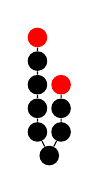
\begin{tikzpicture}[scale=.2]
\node[circle, scale=0.75, fill] (tid0) at (1.5,1.5){};
\node[circle, scale=0.75, fill] (tid1) at (0.75,3){};
\node[circle, scale=0.75, fill] (tid3) at (0.75,4.5){};
\node[circle, scale=0.75, fill] (tid5) at (0.75,6){};
\node[circle, scale=0.75, fill] (tid7) at (0.75,7.5){};
\node[circle, scale=0.75, fill, red] (tid8) at (0.75,9){};
\draw[](tid7) -- (tid8);
\draw[](tid5) -- (tid7);
\draw[](tid3) -- (tid5);
\draw[](tid1) -- (tid3);
\node[circle, scale=0.75, fill] (tid2) at (2.25,3){};
\node[circle, scale=0.75, fill] (tid4) at (2.25,4.5){};
\node[circle, scale=0.75, fill, red] (tid6) at (2.25,6){};
\draw[](tid4) -- (tid6);
\draw[](tid2) -- (tid4);
\draw[](tid0) -- (tid1);
\draw[](tid0) -- (tid2);
\end{tikzpicture}
\nodepart{three}
\footnotesize{6.36719}
\nodepart{four}
\footnotesize{$50\:50$}
};
 & 
\node[draw=black, rectangle split,  rectangle split parts=4] (sn0x188ff90){
\footnotesize{0.222222}
\nodepart{two}
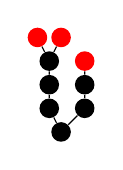
\begin{tikzpicture}[scale=.2]
\node[circle, scale=0.75, fill] (tid0) at (2.25,1.5){};
\node[circle, scale=0.75, fill] (tid1) at (1.5,3){};
\node[circle, scale=0.75, fill] (tid3) at (1.5,4.5){};
\node[circle, scale=0.75, fill] (tid5) at (1.5,6){};
\node[circle, scale=0.75, fill, red] (tid7) at (0.75,7.5){};
\node[circle, scale=0.75, fill, red] (tid8) at (2.25,7.5){};
\draw[](tid5) -- (tid7);
\draw[](tid5) -- (tid8);
\draw[](tid3) -- (tid5);
\draw[](tid1) -- (tid3);
\node[circle, scale=0.75, fill] (tid2) at (3.75,3){};
\node[circle, scale=0.75, fill] (tid4) at (3.75,4.5){};
\node[circle, scale=0.75, fill, red] (tid6) at (3.75,6){};
\draw[](tid4) -- (tid6);
\draw[](tid2) -- (tid4);
\draw[](tid0) -- (tid1);
\draw[](tid0) -- (tid2);
\end{tikzpicture}
\nodepart{three}
\footnotesize{5.95602}
\nodepart{four}
\footnotesize{$33\:67$}
};
 & 
\\
};
\end{scope}
\begin{scope}[yshift=\leveltopIIII cm]
\matrix (line4) [column sep=1cm] {
\node[draw=black, rectangle split,  rectangle split parts=4] (sn0x188c370){
\footnotesize{0.037037}
\nodepart{two}
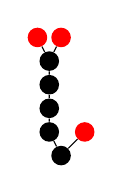
\begin{tikzpicture}[scale=.2]
\node[circle, scale=0.75, fill] (tid0) at (2.25,1.5){};
\node[circle, scale=0.75, fill] (tid1) at (1.5,3){};
\node[circle, scale=0.75, fill] (tid3) at (1.5,4.5){};
\node[circle, scale=0.75, fill] (tid4) at (1.5,6){};
\node[circle, scale=0.75, fill] (tid5) at (1.5,7.5){};
\node[circle, scale=0.75, fill, red] (tid6) at (0.75,9){};
\node[circle, scale=0.75, fill, red] (tid7) at (2.25,9){};
\draw[](tid5) -- (tid6);
\draw[](tid5) -- (tid7);
\draw[](tid4) -- (tid5);
\draw[](tid3) -- (tid4);
\draw[](tid1) -- (tid3);
\node[circle, scale=0.75, fill, red] (tid2) at (3.75,3){};
\draw[](tid0) -- (tid1);
\draw[](tid0) -- (tid2);
\end{tikzpicture}
\nodepart{three}
\footnotesize{6.52083}
\nodepart{four}
\footnotesize{$33\:67$}
};
 & 
\node[draw=black, rectangle split,  rectangle split parts=4] (sn0x188d690){
\footnotesize{0.333333}
\nodepart{two}
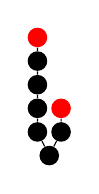
\begin{tikzpicture}[scale=.2]
\node[circle, scale=0.75, fill] (tid0) at (1.5,1.5){};
\node[circle, scale=0.75, fill] (tid1) at (0.75,3){};
\node[circle, scale=0.75, fill] (tid3) at (0.75,4.5){};
\node[circle, scale=0.75, fill] (tid5) at (0.75,6){};
\node[circle, scale=0.75, fill] (tid6) at (0.75,7.5){};
\node[circle, scale=0.75, fill, red] (tid7) at (0.75,9){};
\draw[](tid6) -- (tid7);
\draw[](tid5) -- (tid6);
\draw[](tid3) -- (tid5);
\draw[](tid1) -- (tid3);
\node[circle, scale=0.75, fill] (tid2) at (2.25,3){};
\node[circle, scale=0.75, fill, red] (tid4) at (2.25,4.5){};
\draw[](tid2) -- (tid4);
\draw[](tid0) -- (tid1);
\draw[](tid0) -- (tid2);
\end{tikzpicture}
\nodepart{three}
\footnotesize{6.14062}
\nodepart{four}
\footnotesize{$50\:50$}
};
 & 
\node[draw=black, rectangle split,  rectangle split parts=4] (sn0x188b180){
\footnotesize{0.148148}
\nodepart{two}
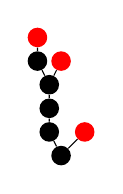
\begin{tikzpicture}[scale=.2]
\node[circle, scale=0.75, fill] (tid0) at (2.25,1.5){};
\node[circle, scale=0.75, fill] (tid1) at (1.5,3){};
\node[circle, scale=0.75, fill] (tid3) at (1.5,4.5){};
\node[circle, scale=0.75, fill] (tid4) at (1.5,6){};
\node[circle, scale=0.75, fill] (tid5) at (0.75,7.5){};
\node[circle, scale=0.75, fill, red] (tid7) at (0.75,9){};
\draw[](tid5) -- (tid7);
\node[circle, scale=0.75, fill, red] (tid6) at (2.25,7.5){};
\draw[](tid4) -- (tid5);
\draw[](tid4) -- (tid6);
\draw[](tid3) -- (tid4);
\draw[](tid1) -- (tid3);
\node[circle, scale=0.75, fill, red] (tid2) at (3.75,3){};
\draw[](tid0) -- (tid1);
\draw[](tid0) -- (tid2);
\end{tikzpicture}
\nodepart{three}
\footnotesize{6.27431}
\nodepart{four}
\footnotesize{$33\:33\:33$}
};
 & 
\node[draw=black, rectangle split,  rectangle split parts=4] (sn0x188de90){
\footnotesize{0.222222}
\nodepart{two}
\begin{tikzpicture}[scale=.2]
\node[circle, scale=0.75, fill] (tid0) at (2.25,1.5){};
\node[circle, scale=0.75, fill] (tid1) at (1.5,3){};
\node[circle, scale=0.75, fill] (tid3) at (1.5,4.5){};
\node[circle, scale=0.75, fill] (tid5) at (1.5,6){};
\node[circle, scale=0.75, fill, red] (tid6) at (0.75,7.5){};
\node[circle, scale=0.75, fill, red] (tid7) at (2.25,7.5){};
\draw[](tid5) -- (tid6);
\draw[](tid5) -- (tid7);
\draw[](tid3) -- (tid5);
\draw[](tid1) -- (tid3);
\node[circle, scale=0.75, fill] (tid2) at (3.75,3){};
\node[circle, scale=0.75, fill, red] (tid4) at (3.75,4.5){};
\draw[](tid2) -- (tid4);
\draw[](tid0) -- (tid1);
\draw[](tid0) -- (tid2);
\end{tikzpicture}
\nodepart{three}
\footnotesize{5.68056}
\nodepart{four}
\footnotesize{$67\:33$}
};
 & 
\node[draw=black, rectangle split,  rectangle split parts=4] (sn0x188f020){
\footnotesize{0.259259}
\nodepart{two}
\begin{tikzpicture}[scale=.2]
\node[circle, scale=0.75, fill] (tid0) at (1.5,1.5){};
\node[circle, scale=0.75, fill] (tid1) at (0.75,3){};
\node[circle, scale=0.75, fill] (tid3) at (0.75,4.5){};
\node[circle, scale=0.75, fill] (tid5) at (0.75,6){};
\node[circle, scale=0.75, fill, red] (tid7) at (0.75,7.5){};
\draw[](tid5) -- (tid7);
\draw[](tid3) -- (tid5);
\draw[](tid1) -- (tid3);
\node[circle, scale=0.75, fill] (tid2) at (2.25,3){};
\node[circle, scale=0.75, fill] (tid4) at (2.25,4.5){};
\node[circle, scale=0.75, fill, red] (tid6) at (2.25,6){};
\draw[](tid4) -- (tid6);
\draw[](tid2) -- (tid4);
\draw[](tid0) -- (tid1);
\draw[](tid0) -- (tid2);
\end{tikzpicture}
\nodepart{three}
\footnotesize{5.59375}
\nodepart{four}
\footnotesize{$50\:50$}
};
 & 
\\
};
\end{scope}
\begin{scope}[yshift=\leveltopIIIII cm]
\matrix (line5) [column sep=1cm] {
\node[draw=black, rectangle split,  rectangle split parts=4] (sn0x1888fa0){
\footnotesize{0.0123457}
\nodepart{two}
\begin{tikzpicture}[scale=.2]
\node[circle, scale=0.75, fill] (tid0) at (1.5,1.5){};
\node[circle, scale=0.75, fill] (tid1) at (1.5,3){};
\node[circle, scale=0.75, fill] (tid2) at (1.5,4.5){};
\node[circle, scale=0.75, fill] (tid3) at (1.5,6){};
\node[circle, scale=0.75, fill] (tid4) at (1.5,7.5){};
\node[circle, scale=0.75, fill, red] (tid5) at (0.75,9){};
\node[circle, scale=0.75, fill, red] (tid6) at (2.25,9){};
\draw[](tid4) -- (tid5);
\draw[](tid4) -- (tid6);
\draw[](tid3) -- (tid4);
\draw[](tid2) -- (tid3);
\draw[](tid1) -- (tid2);
\draw[](tid0) -- (tid1);
\end{tikzpicture}
\nodepart{three}
\footnotesize{6.5}
\nodepart{four}
\footnotesize{$1$}
};
 & 
\node[draw=black, rectangle split,  rectangle split parts=4] (sn0x188ae00){
\footnotesize{0.240741}
\nodepart{two}
\begin{tikzpicture}[scale=.2]
\node[circle, scale=0.75, fill] (tid0) at (1.5,1.5){};
\node[circle, scale=0.75, fill] (tid1) at (0.75,3){};
\node[circle, scale=0.75, fill] (tid3) at (0.75,4.5){};
\node[circle, scale=0.75, fill] (tid4) at (0.75,6){};
\node[circle, scale=0.75, fill] (tid5) at (0.75,7.5){};
\node[circle, scale=0.75, fill, red] (tid6) at (0.75,9){};
\draw[](tid5) -- (tid6);
\draw[](tid4) -- (tid5);
\draw[](tid3) -- (tid4);
\draw[](tid1) -- (tid3);
\node[circle, scale=0.75, fill, red] (tid2) at (2.25,3){};
\draw[](tid0) -- (tid1);
\draw[](tid0) -- (tid2);
\end{tikzpicture}
\nodepart{three}
\footnotesize{6.03125}
\nodepart{four}
\footnotesize{$50\:50$}
};
 & 
\node[draw=black, rectangle split,  rectangle split parts=4] (sn0x188d460){
\footnotesize{0.444444}
\nodepart{two}
\begin{tikzpicture}[scale=.2]
\node[circle, scale=0.75, fill] (tid0) at (1.5,1.5){};
\node[circle, scale=0.75, fill] (tid1) at (0.75,3){};
\node[circle, scale=0.75, fill] (tid3) at (0.75,4.5){};
\node[circle, scale=0.75, fill] (tid5) at (0.75,6){};
\node[circle, scale=0.75, fill, red] (tid6) at (0.75,7.5){};
\draw[](tid5) -- (tid6);
\draw[](tid3) -- (tid5);
\draw[](tid1) -- (tid3);
\node[circle, scale=0.75, fill] (tid2) at (2.25,3){};
\node[circle, scale=0.75, fill, red] (tid4) at (2.25,4.5){};
\draw[](tid2) -- (tid4);
\draw[](tid0) -- (tid1);
\draw[](tid0) -- (tid2);
\end{tikzpicture}
\nodepart{three}
\footnotesize{5.25}
\nodepart{four}
\footnotesize{$50\:50$}
};
 & 
\node[draw=black, rectangle split,  rectangle split parts=4] (sn0x1889a70){
\footnotesize{0.0493827}
\nodepart{two}
\begin{tikzpicture}[scale=.2]
\node[circle, scale=0.75, fill] (tid0) at (1.5,1.5){};
\node[circle, scale=0.75, fill] (tid1) at (1.5,3){};
\node[circle, scale=0.75, fill] (tid2) at (1.5,4.5){};
\node[circle, scale=0.75, fill] (tid3) at (1.5,6){};
\node[circle, scale=0.75, fill] (tid4) at (0.75,7.5){};
\node[circle, scale=0.75, fill, red] (tid6) at (0.75,9){};
\draw[](tid4) -- (tid6);
\node[circle, scale=0.75, fill, red] (tid5) at (2.25,7.5){};
\draw[](tid3) -- (tid4);
\draw[](tid3) -- (tid5);
\draw[](tid2) -- (tid3);
\draw[](tid1) -- (tid2);
\draw[](tid0) -- (tid1);
\end{tikzpicture}
\nodepart{three}
\footnotesize{6.25}
\nodepart{four}
\footnotesize{$50\:50$}
};
 & 
\node[draw=black, rectangle split,  rectangle split parts=4] (sn0x188b630){
\footnotesize{0.123457}
\nodepart{two}
\begin{tikzpicture}[scale=.2]
\node[circle, scale=0.75, fill] (tid0) at (2.25,1.5){};
\node[circle, scale=0.75, fill] (tid1) at (1.5,3){};
\node[circle, scale=0.75, fill] (tid3) at (1.5,4.5){};
\node[circle, scale=0.75, fill] (tid4) at (1.5,6){};
\node[circle, scale=0.75, fill, red] (tid5) at (0.75,7.5){};
\node[circle, scale=0.75, fill, red] (tid6) at (2.25,7.5){};
\draw[](tid4) -- (tid5);
\draw[](tid4) -- (tid6);
\draw[](tid3) -- (tid4);
\draw[](tid1) -- (tid3);
\node[circle, scale=0.75, fill, red] (tid2) at (3.75,3){};
\draw[](tid0) -- (tid1);
\draw[](tid0) -- (tid2);
\end{tikzpicture}
\nodepart{three}
\footnotesize{5.54167}
\nodepart{four}
\footnotesize{$67\:33$}
};
 & 
\node[draw=black, rectangle split,  rectangle split parts=4] (sn0x188fd60){
\footnotesize{0.12963}
\nodepart{two}
\begin{tikzpicture}[scale=.2]
\node[circle, scale=0.75, fill] (tid0) at (1.5,1.5){};
\node[circle, scale=0.75, fill] (tid1) at (0.75,3){};
\node[circle, scale=0.75, fill] (tid3) at (0.75,4.5){};
\node[circle, scale=0.75, fill, red] (tid5) at (0.75,6){};
\draw[](tid3) -- (tid5);
\draw[](tid1) -- (tid3);
\node[circle, scale=0.75, fill] (tid2) at (2.25,3){};
\node[circle, scale=0.75, fill] (tid4) at (2.25,4.5){};
\node[circle, scale=0.75, fill, red] (tid6) at (2.25,6){};
\draw[](tid4) -- (tid6);
\draw[](tid2) -- (tid4);
\draw[](tid0) -- (tid1);
\draw[](tid0) -- (tid2);
\end{tikzpicture}
\nodepart{three}
\footnotesize{4.9375}
\nodepart{four}
\footnotesize{$1$}
};
 & 
\\
};
\end{scope}
\begin{scope}[yshift=\leveltopIIIIII cm]
\matrix (line6) [column sep=1cm] {
\node[draw=black, rectangle split,  rectangle split parts=4] (sn0x1888e50){
\footnotesize{0.157407}
\nodepart{two}
\begin{tikzpicture}[scale=.2]
\node[circle, scale=0.75, fill] (tid0) at (0.75,1.5){};
\node[circle, scale=0.75, fill] (tid1) at (0.75,3){};
\node[circle, scale=0.75, fill] (tid2) at (0.75,4.5){};
\node[circle, scale=0.75, fill] (tid3) at (0.75,6){};
\node[circle, scale=0.75, fill] (tid4) at (0.75,7.5){};
\node[circle, scale=0.75, fill, red] (tid5) at (0.75,9){};
\draw[](tid4) -- (tid5);
\draw[](tid3) -- (tid4);
\draw[](tid2) -- (tid3);
\draw[](tid1) -- (tid2);
\draw[](tid0) -- (tid1);
\end{tikzpicture}
\nodepart{three}
\footnotesize{6}
\nodepart{four}
\footnotesize{$1$}
};
 & 
\node[draw=black, rectangle split,  rectangle split parts=4] (sn0x188acf0){
\footnotesize{0.424897}
\nodepart{two}
\begin{tikzpicture}[scale=.2]
\node[circle, scale=0.75, fill] (tid0) at (1.5,1.5){};
\node[circle, scale=0.75, fill] (tid1) at (0.75,3){};
\node[circle, scale=0.75, fill] (tid3) at (0.75,4.5){};
\node[circle, scale=0.75, fill] (tid4) at (0.75,6){};
\node[circle, scale=0.75, fill, red] (tid5) at (0.75,7.5){};
\draw[](tid4) -- (tid5);
\draw[](tid3) -- (tid4);
\draw[](tid1) -- (tid3);
\node[circle, scale=0.75, fill, red] (tid2) at (2.25,3){};
\draw[](tid0) -- (tid1);
\draw[](tid0) -- (tid2);
\end{tikzpicture}
\nodepart{three}
\footnotesize{5.0625}
\nodepart{four}
\footnotesize{$50\:50$}
};
 & 
\node[draw=black, rectangle split,  rectangle split parts=4] (sn0x188c6a0){
\footnotesize{0.351852}
\nodepart{two}
\begin{tikzpicture}[scale=.2]
\node[circle, scale=0.75, fill] (tid0) at (1.5,1.5){};
\node[circle, scale=0.75, fill] (tid1) at (0.75,3){};
\node[circle, scale=0.75, fill] (tid3) at (0.75,4.5){};
\node[circle, scale=0.75, fill, red] (tid5) at (0.75,6){};
\draw[](tid3) -- (tid5);
\draw[](tid1) -- (tid3);
\node[circle, scale=0.75, fill] (tid2) at (2.25,3){};
\node[circle, scale=0.75, fill, red] (tid4) at (2.25,4.5){};
\draw[](tid2) -- (tid4);
\draw[](tid0) -- (tid1);
\draw[](tid0) -- (tid2);
\end{tikzpicture}
\nodepart{three}
\footnotesize{4.4375}
\nodepart{four}
\footnotesize{$50\:50$}
};
 & 
\node[draw=black, rectangle split,  rectangle split parts=4] (sn0x1889230){
\footnotesize{0.0658436}
\nodepart{two}
\begin{tikzpicture}[scale=.2]
\node[circle, scale=0.75, fill] (tid0) at (1.5,1.5){};
\node[circle, scale=0.75, fill] (tid1) at (1.5,3){};
\node[circle, scale=0.75, fill] (tid2) at (1.5,4.5){};
\node[circle, scale=0.75, fill] (tid3) at (1.5,6){};
\node[circle, scale=0.75, fill, red] (tid4) at (0.75,7.5){};
\node[circle, scale=0.75, fill, red] (tid5) at (2.25,7.5){};
\draw[](tid3) -- (tid4);
\draw[](tid3) -- (tid5);
\draw[](tid2) -- (tid3);
\draw[](tid1) -- (tid2);
\draw[](tid0) -- (tid1);
\end{tikzpicture}
\nodepart{three}
\footnotesize{5.5}
\nodepart{four}
\footnotesize{$1$}
};
 & 
\\
};
\end{scope}
\begin{scope}[yshift=\leveltopIIIIIII cm]
\matrix (line7) [column sep=1cm] {
\node[draw=black, rectangle split,  rectangle split parts=4] (sn0x1888b50){
\footnotesize{0.4357}
\nodepart{two}
\begin{tikzpicture}[scale=.2]
\node[circle, scale=0.75, fill] (tid0) at (0.75,1.5){};
\node[circle, scale=0.75, fill] (tid1) at (0.75,3){};
\node[circle, scale=0.75, fill] (tid2) at (0.75,4.5){};
\node[circle, scale=0.75, fill] (tid3) at (0.75,6){};
\node[circle, scale=0.75, fill, red] (tid4) at (0.75,7.5){};
\draw[](tid3) -- (tid4);
\draw[](tid2) -- (tid3);
\draw[](tid1) -- (tid2);
\draw[](tid0) -- (tid1);
\end{tikzpicture}
\nodepart{three}
\footnotesize{5}
\nodepart{four}
\footnotesize{$1$}
};
 & 
\node[draw=black, rectangle split,  rectangle split parts=4] (sn0x188a9f0){
\footnotesize{0.388375}
\nodepart{two}
\begin{tikzpicture}[scale=.2]
\node[circle, scale=0.75, fill] (tid0) at (1.5,1.5){};
\node[circle, scale=0.75, fill] (tid1) at (0.75,3){};
\node[circle, scale=0.75, fill] (tid3) at (0.75,4.5){};
\node[circle, scale=0.75, fill, red] (tid4) at (0.75,6){};
\draw[](tid3) -- (tid4);
\draw[](tid1) -- (tid3);
\node[circle, scale=0.75, fill, red] (tid2) at (2.25,3){};
\draw[](tid0) -- (tid1);
\draw[](tid0) -- (tid2);
\end{tikzpicture}
\nodepart{three}
\footnotesize{4.125}
\nodepart{four}
\footnotesize{$50\:50$}
};
 & 
\node[draw=black, rectangle split,  rectangle split parts=4] (sn0x188c5b0){
\footnotesize{0.175926}
\nodepart{two}
\begin{tikzpicture}[scale=.2]
\node[circle, scale=0.75, fill] (tid0) at (1.5,1.5){};
\node[circle, scale=0.75, fill] (tid1) at (0.75,3){};
\node[circle, scale=0.75, fill, red] (tid3) at (0.75,4.5){};
\draw[](tid1) -- (tid3);
\node[circle, scale=0.75, fill] (tid2) at (2.25,3){};
\node[circle, scale=0.75, fill, red] (tid4) at (2.25,4.5){};
\draw[](tid2) -- (tid4);
\draw[](tid0) -- (tid1);
\draw[](tid0) -- (tid2);
\end{tikzpicture}
\nodepart{three}
\footnotesize{3.75}
\nodepart{four}
\footnotesize{$1$}
};
 & 
\\
};
\end{scope}
\begin{scope}[yshift=\leveltopIIIIIIII cm]
\matrix (line8) [column sep=1cm] {
\node[draw=black, rectangle split,  rectangle split parts=4] (sn0x1888900){
\footnotesize{0.629887}
\nodepart{two}
\begin{tikzpicture}[scale=.2]
\node[circle, scale=0.75, fill] (tid0) at (0.75,1.5){};
\node[circle, scale=0.75, fill] (tid1) at (0.75,3){};
\node[circle, scale=0.75, fill] (tid2) at (0.75,4.5){};
\node[circle, scale=0.75, fill, red] (tid3) at (0.75,6){};
\draw[](tid2) -- (tid3);
\draw[](tid1) -- (tid2);
\draw[](tid0) -- (tid1);
\end{tikzpicture}
\nodepart{three}
\footnotesize{4}
\nodepart{four}
\footnotesize{$1$}
};
 & 
\node[draw=black, rectangle split,  rectangle split parts=4] (sn0x188a920){
\footnotesize{0.370113}
\nodepart{two}
\begin{tikzpicture}[scale=.2]
\node[circle, scale=0.75, fill] (tid0) at (1.5,1.5){};
\node[circle, scale=0.75, fill] (tid1) at (0.75,3){};
\node[circle, scale=0.75, fill, red] (tid3) at (0.75,4.5){};
\draw[](tid1) -- (tid3);
\node[circle, scale=0.75, fill, red] (tid2) at (2.25,3){};
\draw[](tid0) -- (tid1);
\draw[](tid0) -- (tid2);
\end{tikzpicture}
\nodepart{three}
\footnotesize{3.25}
\nodepart{four}
\footnotesize{$50\:50$}
};
 & 
\\
};
\end{scope}
\begin{scope}[yshift=\leveltopIIIIIIIII cm]
\matrix (line9) [column sep=1cm] {
\node[draw=black, rectangle split,  rectangle split parts=4] (sn0x1888830){
\footnotesize{0.814943}
\nodepart{two}
\begin{tikzpicture}[scale=.2]
\node[circle, scale=0.75, fill] (tid0) at (0.75,1.5){};
\node[circle, scale=0.75, fill] (tid1) at (0.75,3){};
\node[circle, scale=0.75, fill, red] (tid2) at (0.75,4.5){};
\draw[](tid1) -- (tid2);
\draw[](tid0) -- (tid1);
\end{tikzpicture}
\nodepart{three}
\footnotesize{3}
\nodepart{four}
\footnotesize{$1$}
};
 & 
\node[draw=black, rectangle split,  rectangle split parts=4] (sn0x1889c10){
\footnotesize{0.185057}
\nodepart{two}
\begin{tikzpicture}[scale=.2]
\node[circle, scale=0.75, fill] (tid0) at (1.5,1.5){};
\node[circle, scale=0.75, fill, red] (tid1) at (0.75,3){};
\node[circle, scale=0.75, fill, red] (tid2) at (2.25,3){};
\draw[](tid0) -- (tid1);
\draw[](tid0) -- (tid2);
\end{tikzpicture}
\nodepart{three}
\footnotesize{2.5}
\nodepart{four}
\footnotesize{$1$}
};
 & 
\\
};
\end{scope}
\begin{scope}[yshift=\leveltopIIIIIIIIII cm]
\matrix (line10) [column sep=1cm] {
\node[draw=black, rectangle split,  rectangle split parts=4] (sn0x1887520){
\footnotesize{1}
\nodepart{two}
\begin{tikzpicture}[scale=.2]
\node[circle, scale=0.75, fill] (tid0) at (0.75,1.5){};
\node[circle, scale=0.75, fill, red] (tid1) at (0.75,3){};
\draw[](tid0) -- (tid1);
\end{tikzpicture}
\nodepart{three}
\footnotesize{2}
\nodepart{four}
\footnotesize{$1$}
};
 & 
\\
};
\end{scope}
\begin{scope}[yshift=\leveltopIIIIIIIIIII cm]
\matrix (line11) [column sep=1cm] {
\node[draw=black, rectangle split,  rectangle split parts=4] (sn0x1887450){
\footnotesize{1}
\nodepart{two}
\begin{tikzpicture}[scale=.2]
\node[circle, scale=0.75, fill, red] (tid0) at (0.75,1.5){};
\end{tikzpicture}
\nodepart{three}
\footnotesize{1}
\nodepart{four}
\footnotesize{$$}
};
 & 
\\
};
\end{scope}
\begin{scope}[yshift=\leveltopIIIIIIIIIIII cm]
\matrix (line12) [column sep=1cm] {
\\
};
\end{scope}
\draw (sn0x18908d0.south) -- (sn0x188ec30.north);
\draw (sn0x18908d0.south) -- (sn0x18906a0.north);
\draw (sn0x188ec30.south) -- (sn0x188e220.north);
\draw (sn0x188ec30.south) -- (sn0x188d8a0.north);
\draw (sn0x18906a0.south) -- (sn0x188d8a0.north);
\draw (sn0x18906a0.south) -- (sn0x188f0f0.north);
\draw (sn0x18906a0.south) -- (sn0x188ff90.north);
\draw (sn0x188e220.south) -- (sn0x188c370.north);
\draw (sn0x188e220.south) -- (sn0x188d690.north);
\draw (sn0x188d8a0.south) -- (sn0x188b180.north);
\draw (sn0x188d8a0.south) -- (sn0x188d690.north);
\draw (sn0x188d8a0.south) -- (sn0x188de90.north);
\draw (sn0x188f0f0.south) -- (sn0x188d690.north);
\draw (sn0x188f0f0.south) -- (sn0x188f020.north);
\draw (sn0x188ff90.south) -- (sn0x188de90.north);
\draw (sn0x188ff90.south) -- (sn0x188f020.north);
\draw (sn0x188c370.south) -- (sn0x1888fa0.north);
\draw (sn0x188c370.south) -- (sn0x188ae00.north);
\draw (sn0x188d690.south) -- (sn0x188ae00.north);
\draw (sn0x188d690.south) -- (sn0x188d460.north);
\draw (sn0x188b180.south) -- (sn0x1889a70.north);
\draw (sn0x188b180.south) -- (sn0x188ae00.north);
\draw (sn0x188b180.south) -- (sn0x188b630.north);
\draw (sn0x188de90.south) -- (sn0x188b630.north);
\draw (sn0x188de90.south) -- (sn0x188d460.north);
\draw (sn0x188f020.south) -- (sn0x188d460.north);
\draw (sn0x188f020.south) -- (sn0x188fd60.north);
\draw (sn0x1888fa0.south) -- (sn0x1888e50.north);
\draw (sn0x188ae00.south) -- (sn0x1888e50.north);
\draw (sn0x188ae00.south) -- (sn0x188acf0.north);
\draw (sn0x188d460.south) -- (sn0x188acf0.north);
\draw (sn0x188d460.south) -- (sn0x188c6a0.north);
\draw (sn0x1889a70.south) -- (sn0x1888e50.north);
\draw (sn0x1889a70.south) -- (sn0x1889230.north);
\draw (sn0x188b630.south) -- (sn0x1889230.north);
\draw (sn0x188b630.south) -- (sn0x188acf0.north);
\draw (sn0x188fd60.south) -- (sn0x188c6a0.north);
\draw (sn0x1888e50.south) -- (sn0x1888b50.north);
\draw (sn0x188acf0.south) -- (sn0x1888b50.north);
\draw (sn0x188acf0.south) -- (sn0x188a9f0.north);
\draw (sn0x188c6a0.south) -- (sn0x188a9f0.north);
\draw (sn0x188c6a0.south) -- (sn0x188c5b0.north);
\draw (sn0x1889230.south) -- (sn0x1888b50.north);
\draw (sn0x1888b50.south) -- (sn0x1888900.north);
\draw (sn0x188a9f0.south) -- (sn0x1888900.north);
\draw (sn0x188a9f0.south) -- (sn0x188a920.north);
\draw (sn0x188c5b0.south) -- (sn0x188a920.north);
\draw (sn0x1888900.south) -- (sn0x1888830.north);
\draw (sn0x188a920.south) -- (sn0x1888830.north);
\draw (sn0x188a920.south) -- (sn0x1889c10.north);
\draw (sn0x1888830.south) -- (sn0x1887520.north);
\draw (sn0x1889c10.south) -- (sn0x1887520.north);
\draw (sn0x1887520.south) -- (sn0x1887450.north);
\end{tikzpicture}

%%% Local Variables:
%%% TeX-master: "thesis/thesis.tex"
%%% End: 
\renewcommand{\leveltopI}{-15cm + \leveltop}
\renewcommand{\leveltopII}{-15cm + \leveltopI}
\renewcommand{\leveltopIII}{-15cm + \leveltopII}
\renewcommand{\leveltopIIII}{-15cm + \leveltopIII}
\renewcommand{\leveltopIIIII}{-15cm + \leveltopIIII}
\renewcommand{\leveltopIIIIII}{-15cm + \leveltopIIIII}
\renewcommand{\leveltopIIIIIII}{-15cm + \leveltopIIIIII}
\renewcommand{\leveltopIIIIIIII}{-15cm + \leveltopIIIIIII}
\renewcommand{\leveltopIIIIIIIII}{-15cm + \leveltopIIIIIIII}
\renewcommand{\leveltopIIIIIIIIII}{-15cm + \leveltopIIIIIIIII}
\renewcommand{\leveltopIIIIIIIIIII}{-15cm + \leveltopIIIIIIIIII}
\begin{tikzpicture}[scale=.2, anchor=south]
\begin{scope}[yshift=\leveltopI cm]
\matrix (line1) [column sep=1cm] {
\node[draw=black, rectangle split,  rectangle split parts=4] (sn0x1891fa0){
\footnotesize{1}
\nodepart{two}
\begin{tikzpicture}[scale=.2]
\node[circle, scale=0.75, fill] (tid0) at (3,1.5){};
\node[circle, scale=0.75, fill] (tid1) at (2.25,3){};
\node[circle, scale=0.75, fill] (tid3) at (2.25,4.5){};
\node[circle, scale=0.75, fill] (tid5) at (2.25,6){};
\node[circle, scale=0.75, fill] (tid7) at (1.5,7.5){};
\node[circle, scale=0.75, fill, red] (tid9) at (0.75,9){};
\node[circle, scale=0.75, fill] (tid10) at (2.25,9){};
\draw[](tid7) -- (tid9);
\draw[](tid7) -- (tid10);
\node[circle, scale=0.75, fill, red] (tid8) at (3.75,7.5){};
\draw[](tid5) -- (tid7);
\draw[](tid5) -- (tid8);
\draw[](tid3) -- (tid5);
\draw[](tid1) -- (tid3);
\node[circle, scale=0.75, fill] (tid2) at (5.25,3){};
\node[circle, scale=0.75, fill] (tid4) at (5.25,4.5){};
\node[circle, scale=0.75, fill, red] (tid6) at (5.25,6){};
\draw[](tid4) -- (tid6);
\draw[](tid2) -- (tid4);
\draw[](tid0) -- (tid1);
\draw[](tid0) -- (tid2);
\end{tikzpicture}
\nodepart{three}
\footnotesize{7.03938}
\nodepart{four}
\footnotesize{$33\:33\:33$}
};
 & 
\\
};
\end{scope}
\begin{scope}[yshift=\leveltopII cm]
\matrix (line2) [column sep=1cm] {
\node[draw=black, rectangle split,  rectangle split parts=4] (sn0x188ec30){
\footnotesize{0.333333}
\nodepart{two}
\begin{tikzpicture}[scale=.2]
\node[circle, scale=0.75, fill] (tid0) at (3,1.5){};
\node[circle, scale=0.75, fill] (tid1) at (2.25,3){};
\node[circle, scale=0.75, fill] (tid3) at (2.25,4.5){};
\node[circle, scale=0.75, fill] (tid5) at (2.25,6){};
\node[circle, scale=0.75, fill] (tid6) at (1.5,7.5){};
\node[circle, scale=0.75, fill, red] (tid8) at (0.75,9){};
\node[circle, scale=0.75, fill, red] (tid9) at (2.25,9){};
\draw[](tid6) -- (tid8);
\draw[](tid6) -- (tid9);
\node[circle, scale=0.75, fill, red] (tid7) at (3.75,7.5){};
\draw[](tid5) -- (tid6);
\draw[](tid5) -- (tid7);
\draw[](tid3) -- (tid5);
\draw[](tid1) -- (tid3);
\node[circle, scale=0.75, fill] (tid2) at (5.25,3){};
\node[circle, scale=0.75, fill] (tid4) at (5.25,4.5){};
\draw[](tid2) -- (tid4);
\draw[](tid0) -- (tid1);
\draw[](tid0) -- (tid2);
\end{tikzpicture}
\nodepart{three}
\footnotesize{6.77701}
\nodepart{four}
\footnotesize{$33\:67$}
};
 & 
\node[draw=black, rectangle split,  rectangle split parts=4] (sn0x1891ba0){
\footnotesize{0.333333}
\nodepart{two}
\begin{tikzpicture}[scale=.2]
\node[circle, scale=0.75, fill] (tid0) at (2.25,1.5){};
\node[circle, scale=0.75, fill] (tid1) at (1.5,3){};
\node[circle, scale=0.75, fill] (tid3) at (1.5,4.5){};
\node[circle, scale=0.75, fill] (tid5) at (1.5,6){};
\node[circle, scale=0.75, fill] (tid7) at (1.5,7.5){};
\node[circle, scale=0.75, fill, red] (tid8) at (0.75,9){};
\node[circle, scale=0.75, fill, red] (tid9) at (2.25,9){};
\draw[](tid7) -- (tid8);
\draw[](tid7) -- (tid9);
\draw[](tid5) -- (tid7);
\draw[](tid3) -- (tid5);
\draw[](tid1) -- (tid3);
\node[circle, scale=0.75, fill] (tid2) at (3.75,3){};
\node[circle, scale=0.75, fill] (tid4) at (3.75,4.5){};
\node[circle, scale=0.75, fill, red] (tid6) at (3.75,6){};
\draw[](tid4) -- (tid6);
\draw[](tid2) -- (tid4);
\draw[](tid0) -- (tid1);
\draw[](tid0) -- (tid2);
\end{tikzpicture}
\nodepart{three}
\footnotesize{6.77836}
\nodepart{four}
\footnotesize{$33\:67$}
};
 & 
\node[draw=black, rectangle split,  rectangle split parts=4] (sn0x18906a0){
\footnotesize{0.333333}
\nodepart{two}
\begin{tikzpicture}[scale=.2]
\node[circle, scale=0.75, fill] (tid0) at (2.25,1.5){};
\node[circle, scale=0.75, fill] (tid1) at (1.5,3){};
\node[circle, scale=0.75, fill] (tid3) at (1.5,4.5){};
\node[circle, scale=0.75, fill] (tid5) at (1.5,6){};
\node[circle, scale=0.75, fill] (tid7) at (0.75,7.5){};
\node[circle, scale=0.75, fill, red] (tid9) at (0.75,9){};
\draw[](tid7) -- (tid9);
\node[circle, scale=0.75, fill, red] (tid8) at (2.25,7.5){};
\draw[](tid5) -- (tid7);
\draw[](tid5) -- (tid8);
\draw[](tid3) -- (tid5);
\draw[](tid1) -- (tid3);
\node[circle, scale=0.75, fill] (tid2) at (3.75,3){};
\node[circle, scale=0.75, fill] (tid4) at (3.75,4.5){};
\node[circle, scale=0.75, fill, red] (tid6) at (3.75,6){};
\draw[](tid4) -- (tid6);
\draw[](tid2) -- (tid4);
\draw[](tid0) -- (tid1);
\draw[](tid0) -- (tid2);
\end{tikzpicture}
\nodepart{three}
\footnotesize{6.56279}
\nodepart{four}
\footnotesize{$33\:33\:33$}
};
 & 
\\
};
\end{scope}
\begin{scope}[yshift=\leveltopIII cm]
\matrix (line3) [column sep=1cm] {
\node[draw=black, rectangle split,  rectangle split parts=4] (sn0x188e220){
\footnotesize{0.222222}
\nodepart{two}
\begin{tikzpicture}[scale=.2]
\node[circle, scale=0.75, fill] (tid0) at (2.25,1.5){};
\node[circle, scale=0.75, fill] (tid1) at (1.5,3){};
\node[circle, scale=0.75, fill] (tid3) at (1.5,4.5){};
\node[circle, scale=0.75, fill] (tid5) at (1.5,6){};
\node[circle, scale=0.75, fill] (tid6) at (1.5,7.5){};
\node[circle, scale=0.75, fill, red] (tid7) at (0.75,9){};
\node[circle, scale=0.75, fill, red] (tid8) at (2.25,9){};
\draw[](tid6) -- (tid7);
\draw[](tid6) -- (tid8);
\draw[](tid5) -- (tid6);
\draw[](tid3) -- (tid5);
\draw[](tid1) -- (tid3);
\node[circle, scale=0.75, fill] (tid2) at (3.75,3){};
\node[circle, scale=0.75, fill, red] (tid4) at (3.75,4.5){};
\draw[](tid2) -- (tid4);
\draw[](tid0) -- (tid1);
\draw[](tid0) -- (tid2);
\end{tikzpicture}
\nodepart{three}
\footnotesize{6.60069}
\nodepart{four}
\footnotesize{$33\:67$}
};
 & 
\node[draw=black, rectangle split,  rectangle split parts=4] (sn0x188d8a0){
\footnotesize{0.333333}
\nodepart{two}
\begin{tikzpicture}[scale=.2]
\node[circle, scale=0.75, fill] (tid0) at (2.25,1.5){};
\node[circle, scale=0.75, fill] (tid1) at (1.5,3){};
\node[circle, scale=0.75, fill] (tid3) at (1.5,4.5){};
\node[circle, scale=0.75, fill] (tid5) at (1.5,6){};
\node[circle, scale=0.75, fill] (tid6) at (0.75,7.5){};
\node[circle, scale=0.75, fill, red] (tid8) at (0.75,9){};
\draw[](tid6) -- (tid8);
\node[circle, scale=0.75, fill, red] (tid7) at (2.25,7.5){};
\draw[](tid5) -- (tid6);
\draw[](tid5) -- (tid7);
\draw[](tid3) -- (tid5);
\draw[](tid1) -- (tid3);
\node[circle, scale=0.75, fill] (tid2) at (3.75,3){};
\node[circle, scale=0.75, fill, red] (tid4) at (3.75,4.5){};
\draw[](tid2) -- (tid4);
\draw[](tid0) -- (tid1);
\draw[](tid0) -- (tid2);
\end{tikzpicture}
\nodepart{three}
\footnotesize{6.36516}
\nodepart{four}
\footnotesize{$33\:33\:33$}
};
 & 
\node[draw=black, rectangle split,  rectangle split parts=4] (sn0x188f0f0){
\footnotesize{0.333333}
\nodepart{two}
\begin{tikzpicture}[scale=.2]
\node[circle, scale=0.75, fill] (tid0) at (1.5,1.5){};
\node[circle, scale=0.75, fill] (tid1) at (0.75,3){};
\node[circle, scale=0.75, fill] (tid3) at (0.75,4.5){};
\node[circle, scale=0.75, fill] (tid5) at (0.75,6){};
\node[circle, scale=0.75, fill] (tid7) at (0.75,7.5){};
\node[circle, scale=0.75, fill, red] (tid8) at (0.75,9){};
\draw[](tid7) -- (tid8);
\draw[](tid5) -- (tid7);
\draw[](tid3) -- (tid5);
\draw[](tid1) -- (tid3);
\node[circle, scale=0.75, fill] (tid2) at (2.25,3){};
\node[circle, scale=0.75, fill] (tid4) at (2.25,4.5){};
\node[circle, scale=0.75, fill, red] (tid6) at (2.25,6){};
\draw[](tid4) -- (tid6);
\draw[](tid2) -- (tid4);
\draw[](tid0) -- (tid1);
\draw[](tid0) -- (tid2);
\end{tikzpicture}
\nodepart{three}
\footnotesize{6.36719}
\nodepart{four}
\footnotesize{$50\:50$}
};
 & 
\node[draw=black, rectangle split,  rectangle split parts=4] (sn0x188ff90){
\footnotesize{0.111111}
\nodepart{two}
\begin{tikzpicture}[scale=.2]
\node[circle, scale=0.75, fill] (tid0) at (2.25,1.5){};
\node[circle, scale=0.75, fill] (tid1) at (1.5,3){};
\node[circle, scale=0.75, fill] (tid3) at (1.5,4.5){};
\node[circle, scale=0.75, fill] (tid5) at (1.5,6){};
\node[circle, scale=0.75, fill, red] (tid7) at (0.75,7.5){};
\node[circle, scale=0.75, fill, red] (tid8) at (2.25,7.5){};
\draw[](tid5) -- (tid7);
\draw[](tid5) -- (tid8);
\draw[](tid3) -- (tid5);
\draw[](tid1) -- (tid3);
\node[circle, scale=0.75, fill] (tid2) at (3.75,3){};
\node[circle, scale=0.75, fill] (tid4) at (3.75,4.5){};
\node[circle, scale=0.75, fill, red] (tid6) at (3.75,6){};
\draw[](tid4) -- (tid6);
\draw[](tid2) -- (tid4);
\draw[](tid0) -- (tid1);
\draw[](tid0) -- (tid2);
\end{tikzpicture}
\nodepart{three}
\footnotesize{5.95602}
\nodepart{four}
\footnotesize{$33\:67$}
};
 & 
\\
};
\end{scope}
\begin{scope}[yshift=\leveltopIIII cm]
\matrix (line4) [column sep=1cm] {
\node[draw=black, rectangle split,  rectangle split parts=4] (sn0x188c370){
\footnotesize{0.0740741}
\nodepart{two}
\begin{tikzpicture}[scale=.2]
\node[circle, scale=0.75, fill] (tid0) at (2.25,1.5){};
\node[circle, scale=0.75, fill] (tid1) at (1.5,3){};
\node[circle, scale=0.75, fill] (tid3) at (1.5,4.5){};
\node[circle, scale=0.75, fill] (tid4) at (1.5,6){};
\node[circle, scale=0.75, fill] (tid5) at (1.5,7.5){};
\node[circle, scale=0.75, fill, red] (tid6) at (0.75,9){};
\node[circle, scale=0.75, fill, red] (tid7) at (2.25,9){};
\draw[](tid5) -- (tid6);
\draw[](tid5) -- (tid7);
\draw[](tid4) -- (tid5);
\draw[](tid3) -- (tid4);
\draw[](tid1) -- (tid3);
\node[circle, scale=0.75, fill, red] (tid2) at (3.75,3){};
\draw[](tid0) -- (tid1);
\draw[](tid0) -- (tid2);
\end{tikzpicture}
\nodepart{three}
\footnotesize{6.52083}
\nodepart{four}
\footnotesize{$33\:67$}
};
 & 
\node[draw=black, rectangle split,  rectangle split parts=4] (sn0x188d690){
\footnotesize{0.425926}
\nodepart{two}
\begin{tikzpicture}[scale=.2]
\node[circle, scale=0.75, fill] (tid0) at (1.5,1.5){};
\node[circle, scale=0.75, fill] (tid1) at (0.75,3){};
\node[circle, scale=0.75, fill] (tid3) at (0.75,4.5){};
\node[circle, scale=0.75, fill] (tid5) at (0.75,6){};
\node[circle, scale=0.75, fill] (tid6) at (0.75,7.5){};
\node[circle, scale=0.75, fill, red] (tid7) at (0.75,9){};
\draw[](tid6) -- (tid7);
\draw[](tid5) -- (tid6);
\draw[](tid3) -- (tid5);
\draw[](tid1) -- (tid3);
\node[circle, scale=0.75, fill] (tid2) at (2.25,3){};
\node[circle, scale=0.75, fill, red] (tid4) at (2.25,4.5){};
\draw[](tid2) -- (tid4);
\draw[](tid0) -- (tid1);
\draw[](tid0) -- (tid2);
\end{tikzpicture}
\nodepart{three}
\footnotesize{6.14062}
\nodepart{four}
\footnotesize{$50\:50$}
};
 & 
\node[draw=black, rectangle split,  rectangle split parts=4] (sn0x188b180){
\footnotesize{0.111111}
\nodepart{two}
\begin{tikzpicture}[scale=.2]
\node[circle, scale=0.75, fill] (tid0) at (2.25,1.5){};
\node[circle, scale=0.75, fill] (tid1) at (1.5,3){};
\node[circle, scale=0.75, fill] (tid3) at (1.5,4.5){};
\node[circle, scale=0.75, fill] (tid4) at (1.5,6){};
\node[circle, scale=0.75, fill] (tid5) at (0.75,7.5){};
\node[circle, scale=0.75, fill, red] (tid7) at (0.75,9){};
\draw[](tid5) -- (tid7);
\node[circle, scale=0.75, fill, red] (tid6) at (2.25,7.5){};
\draw[](tid4) -- (tid5);
\draw[](tid4) -- (tid6);
\draw[](tid3) -- (tid4);
\draw[](tid1) -- (tid3);
\node[circle, scale=0.75, fill, red] (tid2) at (3.75,3){};
\draw[](tid0) -- (tid1);
\draw[](tid0) -- (tid2);
\end{tikzpicture}
\nodepart{three}
\footnotesize{6.27431}
\nodepart{four}
\footnotesize{$33\:33\:33$}
};
 & 
\node[draw=black, rectangle split,  rectangle split parts=4] (sn0x188de90){
\footnotesize{0.148148}
\nodepart{two}
\begin{tikzpicture}[scale=.2]
\node[circle, scale=0.75, fill] (tid0) at (2.25,1.5){};
\node[circle, scale=0.75, fill] (tid1) at (1.5,3){};
\node[circle, scale=0.75, fill] (tid3) at (1.5,4.5){};
\node[circle, scale=0.75, fill] (tid5) at (1.5,6){};
\node[circle, scale=0.75, fill, red] (tid6) at (0.75,7.5){};
\node[circle, scale=0.75, fill, red] (tid7) at (2.25,7.5){};
\draw[](tid5) -- (tid6);
\draw[](tid5) -- (tid7);
\draw[](tid3) -- (tid5);
\draw[](tid1) -- (tid3);
\node[circle, scale=0.75, fill] (tid2) at (3.75,3){};
\node[circle, scale=0.75, fill, red] (tid4) at (3.75,4.5){};
\draw[](tid2) -- (tid4);
\draw[](tid0) -- (tid1);
\draw[](tid0) -- (tid2);
\end{tikzpicture}
\nodepart{three}
\footnotesize{5.68056}
\nodepart{four}
\footnotesize{$67\:33$}
};
 & 
\node[draw=black, rectangle split,  rectangle split parts=4] (sn0x188f020){
\footnotesize{0.240741}
\nodepart{two}
\begin{tikzpicture}[scale=.2]
\node[circle, scale=0.75, fill] (tid0) at (1.5,1.5){};
\node[circle, scale=0.75, fill] (tid1) at (0.75,3){};
\node[circle, scale=0.75, fill] (tid3) at (0.75,4.5){};
\node[circle, scale=0.75, fill] (tid5) at (0.75,6){};
\node[circle, scale=0.75, fill, red] (tid7) at (0.75,7.5){};
\draw[](tid5) -- (tid7);
\draw[](tid3) -- (tid5);
\draw[](tid1) -- (tid3);
\node[circle, scale=0.75, fill] (tid2) at (2.25,3){};
\node[circle, scale=0.75, fill] (tid4) at (2.25,4.5){};
\node[circle, scale=0.75, fill, red] (tid6) at (2.25,6){};
\draw[](tid4) -- (tid6);
\draw[](tid2) -- (tid4);
\draw[](tid0) -- (tid1);
\draw[](tid0) -- (tid2);
\end{tikzpicture}
\nodepart{three}
\footnotesize{5.59375}
\nodepart{four}
\footnotesize{$50\:50$}
};
 & 
\\
};
\end{scope}
\begin{scope}[yshift=\leveltopIIIII cm]
\matrix (line5) [column sep=1cm] {
\node[draw=black, rectangle split,  rectangle split parts=4] (sn0x1888fa0){
\footnotesize{0.0246914}
\nodepart{two}
\begin{tikzpicture}[scale=.2]
\node[circle, scale=0.75, fill] (tid0) at (1.5,1.5){};
\node[circle, scale=0.75, fill] (tid1) at (1.5,3){};
\node[circle, scale=0.75, fill] (tid2) at (1.5,4.5){};
\node[circle, scale=0.75, fill] (tid3) at (1.5,6){};
\node[circle, scale=0.75, fill] (tid4) at (1.5,7.5){};
\node[circle, scale=0.75, fill, red] (tid5) at (0.75,9){};
\node[circle, scale=0.75, fill, red] (tid6) at (2.25,9){};
\draw[](tid4) -- (tid5);
\draw[](tid4) -- (tid6);
\draw[](tid3) -- (tid4);
\draw[](tid2) -- (tid3);
\draw[](tid1) -- (tid2);
\draw[](tid0) -- (tid1);
\end{tikzpicture}
\nodepart{three}
\footnotesize{6.5}
\nodepart{four}
\footnotesize{$1$}
};
 & 
\node[draw=black, rectangle split,  rectangle split parts=4] (sn0x188ae00){
\footnotesize{0.299383}
\nodepart{two}
\begin{tikzpicture}[scale=.2]
\node[circle, scale=0.75, fill] (tid0) at (1.5,1.5){};
\node[circle, scale=0.75, fill] (tid1) at (0.75,3){};
\node[circle, scale=0.75, fill] (tid3) at (0.75,4.5){};
\node[circle, scale=0.75, fill] (tid4) at (0.75,6){};
\node[circle, scale=0.75, fill] (tid5) at (0.75,7.5){};
\node[circle, scale=0.75, fill, red] (tid6) at (0.75,9){};
\draw[](tid5) -- (tid6);
\draw[](tid4) -- (tid5);
\draw[](tid3) -- (tid4);
\draw[](tid1) -- (tid3);
\node[circle, scale=0.75, fill, red] (tid2) at (2.25,3){};
\draw[](tid0) -- (tid1);
\draw[](tid0) -- (tid2);
\end{tikzpicture}
\nodepart{three}
\footnotesize{6.03125}
\nodepart{four}
\footnotesize{$50\:50$}
};
 & 
\node[draw=black, rectangle split,  rectangle split parts=4] (sn0x188d460){
\footnotesize{0.432099}
\nodepart{two}
\begin{tikzpicture}[scale=.2]
\node[circle, scale=0.75, fill] (tid0) at (1.5,1.5){};
\node[circle, scale=0.75, fill] (tid1) at (0.75,3){};
\node[circle, scale=0.75, fill] (tid3) at (0.75,4.5){};
\node[circle, scale=0.75, fill] (tid5) at (0.75,6){};
\node[circle, scale=0.75, fill, red] (tid6) at (0.75,7.5){};
\draw[](tid5) -- (tid6);
\draw[](tid3) -- (tid5);
\draw[](tid1) -- (tid3);
\node[circle, scale=0.75, fill] (tid2) at (2.25,3){};
\node[circle, scale=0.75, fill, red] (tid4) at (2.25,4.5){};
\draw[](tid2) -- (tid4);
\draw[](tid0) -- (tid1);
\draw[](tid0) -- (tid2);
\end{tikzpicture}
\nodepart{three}
\footnotesize{5.25}
\nodepart{four}
\footnotesize{$50\:50$}
};
 & 
\node[draw=black, rectangle split,  rectangle split parts=4] (sn0x1889a70){
\footnotesize{0.037037}
\nodepart{two}
\begin{tikzpicture}[scale=.2]
\node[circle, scale=0.75, fill] (tid0) at (1.5,1.5){};
\node[circle, scale=0.75, fill] (tid1) at (1.5,3){};
\node[circle, scale=0.75, fill] (tid2) at (1.5,4.5){};
\node[circle, scale=0.75, fill] (tid3) at (1.5,6){};
\node[circle, scale=0.75, fill] (tid4) at (0.75,7.5){};
\node[circle, scale=0.75, fill, red] (tid6) at (0.75,9){};
\draw[](tid4) -- (tid6);
\node[circle, scale=0.75, fill, red] (tid5) at (2.25,7.5){};
\draw[](tid3) -- (tid4);
\draw[](tid3) -- (tid5);
\draw[](tid2) -- (tid3);
\draw[](tid1) -- (tid2);
\draw[](tid0) -- (tid1);
\end{tikzpicture}
\nodepart{three}
\footnotesize{6.25}
\nodepart{four}
\footnotesize{$50\:50$}
};
 & 
\node[draw=black, rectangle split,  rectangle split parts=4] (sn0x188b630){
\footnotesize{0.0864198}
\nodepart{two}
\begin{tikzpicture}[scale=.2]
\node[circle, scale=0.75, fill] (tid0) at (2.25,1.5){};
\node[circle, scale=0.75, fill] (tid1) at (1.5,3){};
\node[circle, scale=0.75, fill] (tid3) at (1.5,4.5){};
\node[circle, scale=0.75, fill] (tid4) at (1.5,6){};
\node[circle, scale=0.75, fill, red] (tid5) at (0.75,7.5){};
\node[circle, scale=0.75, fill, red] (tid6) at (2.25,7.5){};
\draw[](tid4) -- (tid5);
\draw[](tid4) -- (tid6);
\draw[](tid3) -- (tid4);
\draw[](tid1) -- (tid3);
\node[circle, scale=0.75, fill, red] (tid2) at (3.75,3){};
\draw[](tid0) -- (tid1);
\draw[](tid0) -- (tid2);
\end{tikzpicture}
\nodepart{three}
\footnotesize{5.54167}
\nodepart{four}
\footnotesize{$67\:33$}
};
 & 
\node[draw=black, rectangle split,  rectangle split parts=4] (sn0x188fd60){
\footnotesize{0.12037}
\nodepart{two}
\begin{tikzpicture}[scale=.2]
\node[circle, scale=0.75, fill] (tid0) at (1.5,1.5){};
\node[circle, scale=0.75, fill] (tid1) at (0.75,3){};
\node[circle, scale=0.75, fill] (tid3) at (0.75,4.5){};
\node[circle, scale=0.75, fill, red] (tid5) at (0.75,6){};
\draw[](tid3) -- (tid5);
\draw[](tid1) -- (tid3);
\node[circle, scale=0.75, fill] (tid2) at (2.25,3){};
\node[circle, scale=0.75, fill] (tid4) at (2.25,4.5){};
\node[circle, scale=0.75, fill, red] (tid6) at (2.25,6){};
\draw[](tid4) -- (tid6);
\draw[](tid2) -- (tid4);
\draw[](tid0) -- (tid1);
\draw[](tid0) -- (tid2);
\end{tikzpicture}
\nodepart{three}
\footnotesize{4.9375}
\nodepart{four}
\footnotesize{$1$}
};
 & 
\\
};
\end{scope}
\begin{scope}[yshift=\leveltopIIIIII cm]
\matrix (line6) [column sep=1cm] {
\node[draw=black, rectangle split,  rectangle split parts=4] (sn0x1888e50){
\footnotesize{0.192901}
\nodepart{two}
\begin{tikzpicture}[scale=.2]
\node[circle, scale=0.75, fill] (tid0) at (0.75,1.5){};
\node[circle, scale=0.75, fill] (tid1) at (0.75,3){};
\node[circle, scale=0.75, fill] (tid2) at (0.75,4.5){};
\node[circle, scale=0.75, fill] (tid3) at (0.75,6){};
\node[circle, scale=0.75, fill] (tid4) at (0.75,7.5){};
\node[circle, scale=0.75, fill, red] (tid5) at (0.75,9){};
\draw[](tid4) -- (tid5);
\draw[](tid3) -- (tid4);
\draw[](tid2) -- (tid3);
\draw[](tid1) -- (tid2);
\draw[](tid0) -- (tid1);
\end{tikzpicture}
\nodepart{three}
\footnotesize{6}
\nodepart{four}
\footnotesize{$1$}
};
 & 
\node[draw=black, rectangle split,  rectangle split parts=4] (sn0x188acf0){
\footnotesize{0.423354}
\nodepart{two}
\begin{tikzpicture}[scale=.2]
\node[circle, scale=0.75, fill] (tid0) at (1.5,1.5){};
\node[circle, scale=0.75, fill] (tid1) at (0.75,3){};
\node[circle, scale=0.75, fill] (tid3) at (0.75,4.5){};
\node[circle, scale=0.75, fill] (tid4) at (0.75,6){};
\node[circle, scale=0.75, fill, red] (tid5) at (0.75,7.5){};
\draw[](tid4) -- (tid5);
\draw[](tid3) -- (tid4);
\draw[](tid1) -- (tid3);
\node[circle, scale=0.75, fill, red] (tid2) at (2.25,3){};
\draw[](tid0) -- (tid1);
\draw[](tid0) -- (tid2);
\end{tikzpicture}
\nodepart{three}
\footnotesize{5.0625}
\nodepart{four}
\footnotesize{$50\:50$}
};
 & 
\node[draw=black, rectangle split,  rectangle split parts=4] (sn0x188c6a0){
\footnotesize{0.33642}
\nodepart{two}
\begin{tikzpicture}[scale=.2]
\node[circle, scale=0.75, fill] (tid0) at (1.5,1.5){};
\node[circle, scale=0.75, fill] (tid1) at (0.75,3){};
\node[circle, scale=0.75, fill] (tid3) at (0.75,4.5){};
\node[circle, scale=0.75, fill, red] (tid5) at (0.75,6){};
\draw[](tid3) -- (tid5);
\draw[](tid1) -- (tid3);
\node[circle, scale=0.75, fill] (tid2) at (2.25,3){};
\node[circle, scale=0.75, fill, red] (tid4) at (2.25,4.5){};
\draw[](tid2) -- (tid4);
\draw[](tid0) -- (tid1);
\draw[](tid0) -- (tid2);
\end{tikzpicture}
\nodepart{three}
\footnotesize{4.4375}
\nodepart{four}
\footnotesize{$50\:50$}
};
 & 
\node[draw=black, rectangle split,  rectangle split parts=4] (sn0x1889230){
\footnotesize{0.0473251}
\nodepart{two}
\begin{tikzpicture}[scale=.2]
\node[circle, scale=0.75, fill] (tid0) at (1.5,1.5){};
\node[circle, scale=0.75, fill] (tid1) at (1.5,3){};
\node[circle, scale=0.75, fill] (tid2) at (1.5,4.5){};
\node[circle, scale=0.75, fill] (tid3) at (1.5,6){};
\node[circle, scale=0.75, fill, red] (tid4) at (0.75,7.5){};
\node[circle, scale=0.75, fill, red] (tid5) at (2.25,7.5){};
\draw[](tid3) -- (tid4);
\draw[](tid3) -- (tid5);
\draw[](tid2) -- (tid3);
\draw[](tid1) -- (tid2);
\draw[](tid0) -- (tid1);
\end{tikzpicture}
\nodepart{three}
\footnotesize{5.5}
\nodepart{four}
\footnotesize{$1$}
};
 & 
\\
};
\end{scope}
\begin{scope}[yshift=\leveltopIIIIIII cm]
\matrix (line7) [column sep=1cm] {
\node[draw=black, rectangle split,  rectangle split parts=4] (sn0x1888b50){
\footnotesize{0.451903}
\nodepart{two}
\begin{tikzpicture}[scale=.2]
\node[circle, scale=0.75, fill] (tid0) at (0.75,1.5){};
\node[circle, scale=0.75, fill] (tid1) at (0.75,3){};
\node[circle, scale=0.75, fill] (tid2) at (0.75,4.5){};
\node[circle, scale=0.75, fill] (tid3) at (0.75,6){};
\node[circle, scale=0.75, fill, red] (tid4) at (0.75,7.5){};
\draw[](tid3) -- (tid4);
\draw[](tid2) -- (tid3);
\draw[](tid1) -- (tid2);
\draw[](tid0) -- (tid1);
\end{tikzpicture}
\nodepart{three}
\footnotesize{5}
\nodepart{four}
\footnotesize{$1$}
};
 & 
\node[draw=black, rectangle split,  rectangle split parts=4] (sn0x188a9f0){
\footnotesize{0.379887}
\nodepart{two}
\begin{tikzpicture}[scale=.2]
\node[circle, scale=0.75, fill] (tid0) at (1.5,1.5){};
\node[circle, scale=0.75, fill] (tid1) at (0.75,3){};
\node[circle, scale=0.75, fill] (tid3) at (0.75,4.5){};
\node[circle, scale=0.75, fill, red] (tid4) at (0.75,6){};
\draw[](tid3) -- (tid4);
\draw[](tid1) -- (tid3);
\node[circle, scale=0.75, fill, red] (tid2) at (2.25,3){};
\draw[](tid0) -- (tid1);
\draw[](tid0) -- (tid2);
\end{tikzpicture}
\nodepart{three}
\footnotesize{4.125}
\nodepart{four}
\footnotesize{$50\:50$}
};
 & 
\node[draw=black, rectangle split,  rectangle split parts=4] (sn0x188c5b0){
\footnotesize{0.16821}
\nodepart{two}
\begin{tikzpicture}[scale=.2]
\node[circle, scale=0.75, fill] (tid0) at (1.5,1.5){};
\node[circle, scale=0.75, fill] (tid1) at (0.75,3){};
\node[circle, scale=0.75, fill, red] (tid3) at (0.75,4.5){};
\draw[](tid1) -- (tid3);
\node[circle, scale=0.75, fill] (tid2) at (2.25,3){};
\node[circle, scale=0.75, fill, red] (tid4) at (2.25,4.5){};
\draw[](tid2) -- (tid4);
\draw[](tid0) -- (tid1);
\draw[](tid0) -- (tid2);
\end{tikzpicture}
\nodepart{three}
\footnotesize{3.75}
\nodepart{four}
\footnotesize{$1$}
};
 & 
\\
};
\end{scope}
\begin{scope}[yshift=\leveltopIIIIIIII cm]
\matrix (line8) [column sep=1cm] {
\node[draw=black, rectangle split,  rectangle split parts=4] (sn0x1888900){
\footnotesize{0.641847}
\nodepart{two}
\begin{tikzpicture}[scale=.2]
\node[circle, scale=0.75, fill] (tid0) at (0.75,1.5){};
\node[circle, scale=0.75, fill] (tid1) at (0.75,3){};
\node[circle, scale=0.75, fill] (tid2) at (0.75,4.5){};
\node[circle, scale=0.75, fill, red] (tid3) at (0.75,6){};
\draw[](tid2) -- (tid3);
\draw[](tid1) -- (tid2);
\draw[](tid0) -- (tid1);
\end{tikzpicture}
\nodepart{three}
\footnotesize{4}
\nodepart{four}
\footnotesize{$1$}
};
 & 
\node[draw=black, rectangle split,  rectangle split parts=4] (sn0x188a920){
\footnotesize{0.358153}
\nodepart{two}
\begin{tikzpicture}[scale=.2]
\node[circle, scale=0.75, fill] (tid0) at (1.5,1.5){};
\node[circle, scale=0.75, fill] (tid1) at (0.75,3){};
\node[circle, scale=0.75, fill, red] (tid3) at (0.75,4.5){};
\draw[](tid1) -- (tid3);
\node[circle, scale=0.75, fill, red] (tid2) at (2.25,3){};
\draw[](tid0) -- (tid1);
\draw[](tid0) -- (tid2);
\end{tikzpicture}
\nodepart{three}
\footnotesize{3.25}
\nodepart{four}
\footnotesize{$50\:50$}
};
 & 
\\
};
\end{scope}
\begin{scope}[yshift=\leveltopIIIIIIIII cm]
\matrix (line9) [column sep=1cm] {
\node[draw=black, rectangle split,  rectangle split parts=4] (sn0x1888830){
\footnotesize{0.820923}
\nodepart{two}
\begin{tikzpicture}[scale=.2]
\node[circle, scale=0.75, fill] (tid0) at (0.75,1.5){};
\node[circle, scale=0.75, fill] (tid1) at (0.75,3){};
\node[circle, scale=0.75, fill, red] (tid2) at (0.75,4.5){};
\draw[](tid1) -- (tid2);
\draw[](tid0) -- (tid1);
\end{tikzpicture}
\nodepart{three}
\footnotesize{3}
\nodepart{four}
\footnotesize{$1$}
};
 & 
\node[draw=black, rectangle split,  rectangle split parts=4] (sn0x1889c10){
\footnotesize{0.179077}
\nodepart{two}
\begin{tikzpicture}[scale=.2]
\node[circle, scale=0.75, fill] (tid0) at (1.5,1.5){};
\node[circle, scale=0.75, fill, red] (tid1) at (0.75,3){};
\node[circle, scale=0.75, fill, red] (tid2) at (2.25,3){};
\draw[](tid0) -- (tid1);
\draw[](tid0) -- (tid2);
\end{tikzpicture}
\nodepart{three}
\footnotesize{2.5}
\nodepart{four}
\footnotesize{$1$}
};
 & 
\\
};
\end{scope}
\begin{scope}[yshift=\leveltopIIIIIIIIII cm]
\matrix (line10) [column sep=1cm] {
\node[draw=black, rectangle split,  rectangle split parts=4] (sn0x1887520){
\footnotesize{1}
\nodepart{two}
\begin{tikzpicture}[scale=.2]
\node[circle, scale=0.75, fill] (tid0) at (0.75,1.5){};
\node[circle, scale=0.75, fill, red] (tid1) at (0.75,3){};
\draw[](tid0) -- (tid1);
\end{tikzpicture}
\nodepart{three}
\footnotesize{2}
\nodepart{four}
\footnotesize{$1$}
};
 & 
\\
};
\end{scope}
\begin{scope}[yshift=\leveltopIIIIIIIIIII cm]
\matrix (line11) [column sep=1cm] {
\node[draw=black, rectangle split,  rectangle split parts=4] (sn0x1887450){
\footnotesize{1}
\nodepart{two}
\begin{tikzpicture}[scale=.2]
\node[circle, scale=0.75, fill, red] (tid0) at (0.75,1.5){};
\end{tikzpicture}
\nodepart{three}
\footnotesize{1}
\nodepart{four}
\footnotesize{$$}
};
 & 
\\
};
\end{scope}
\begin{scope}[yshift=\leveltopIIIIIIIIIIII cm]
\matrix (line12) [column sep=1cm] {
\\
};
\end{scope}
\draw (sn0x1891fa0.south) -- (sn0x188ec30.north);
\draw (sn0x1891fa0.south) -- (sn0x1891ba0.north);
\draw (sn0x1891fa0.south) -- (sn0x18906a0.north);
\draw (sn0x188ec30.south) -- (sn0x188e220.north);
\draw (sn0x188ec30.south) -- (sn0x188d8a0.north);
\draw (sn0x1891ba0.south) -- (sn0x188e220.north);
\draw (sn0x1891ba0.south) -- (sn0x188f0f0.north);
\draw (sn0x18906a0.south) -- (sn0x188d8a0.north);
\draw (sn0x18906a0.south) -- (sn0x188f0f0.north);
\draw (sn0x18906a0.south) -- (sn0x188ff90.north);
\draw (sn0x188e220.south) -- (sn0x188c370.north);
\draw (sn0x188e220.south) -- (sn0x188d690.north);
\draw (sn0x188d8a0.south) -- (sn0x188b180.north);
\draw (sn0x188d8a0.south) -- (sn0x188d690.north);
\draw (sn0x188d8a0.south) -- (sn0x188de90.north);
\draw (sn0x188f0f0.south) -- (sn0x188d690.north);
\draw (sn0x188f0f0.south) -- (sn0x188f020.north);
\draw (sn0x188ff90.south) -- (sn0x188de90.north);
\draw (sn0x188ff90.south) -- (sn0x188f020.north);
\draw (sn0x188c370.south) -- (sn0x1888fa0.north);
\draw (sn0x188c370.south) -- (sn0x188ae00.north);
\draw (sn0x188d690.south) -- (sn0x188ae00.north);
\draw (sn0x188d690.south) -- (sn0x188d460.north);
\draw (sn0x188b180.south) -- (sn0x1889a70.north);
\draw (sn0x188b180.south) -- (sn0x188ae00.north);
\draw (sn0x188b180.south) -- (sn0x188b630.north);
\draw (sn0x188de90.south) -- (sn0x188b630.north);
\draw (sn0x188de90.south) -- (sn0x188d460.north);
\draw (sn0x188f020.south) -- (sn0x188d460.north);
\draw (sn0x188f020.south) -- (sn0x188fd60.north);
\draw (sn0x1888fa0.south) -- (sn0x1888e50.north);
\draw (sn0x188ae00.south) -- (sn0x1888e50.north);
\draw (sn0x188ae00.south) -- (sn0x188acf0.north);
\draw (sn0x188d460.south) -- (sn0x188acf0.north);
\draw (sn0x188d460.south) -- (sn0x188c6a0.north);
\draw (sn0x1889a70.south) -- (sn0x1888e50.north);
\draw (sn0x1889a70.south) -- (sn0x1889230.north);
\draw (sn0x188b630.south) -- (sn0x1889230.north);
\draw (sn0x188b630.south) -- (sn0x188acf0.north);
\draw (sn0x188fd60.south) -- (sn0x188c6a0.north);
\draw (sn0x1888e50.south) -- (sn0x1888b50.north);
\draw (sn0x188acf0.south) -- (sn0x1888b50.north);
\draw (sn0x188acf0.south) -- (sn0x188a9f0.north);
\draw (sn0x188c6a0.south) -- (sn0x188a9f0.north);
\draw (sn0x188c6a0.south) -- (sn0x188c5b0.north);
\draw (sn0x1889230.south) -- (sn0x1888b50.north);
\draw (sn0x1888b50.south) -- (sn0x1888900.north);
\draw (sn0x188a9f0.south) -- (sn0x1888900.north);
\draw (sn0x188a9f0.south) -- (sn0x188a920.north);
\draw (sn0x188c5b0.south) -- (sn0x188a920.north);
\draw (sn0x1888900.south) -- (sn0x1888830.north);
\draw (sn0x188a920.south) -- (sn0x1888830.north);
\draw (sn0x188a920.south) -- (sn0x1889c10.north);
\draw (sn0x1888830.south) -- (sn0x1887520.north);
\draw (sn0x1889c10.south) -- (sn0x1887520.north);
\draw (sn0x1887520.south) -- (sn0x1887450.north);
\end{tikzpicture}

%%% Local Variables:
%%% TeX-master: "thesis/thesis.tex"
%%% End: 
\renewcommand{\leveltopI}{-15cm + \leveltop}
\renewcommand{\leveltopII}{-15cm + \leveltopI}
\renewcommand{\leveltopIII}{-15cm + \leveltopII}
\renewcommand{\leveltopIIII}{-15cm + \leveltopIII}
\renewcommand{\leveltopIIIII}{-15cm + \leveltopIIII}
\renewcommand{\leveltopIIIIII}{-15cm + \leveltopIIIII}
\renewcommand{\leveltopIIIIIII}{-15cm + \leveltopIIIIII}
\renewcommand{\leveltopIIIIIIII}{-15cm + \leveltopIIIIIII}
\renewcommand{\leveltopIIIIIIIII}{-15cm + \leveltopIIIIIIII}
\renewcommand{\leveltopIIIIIIIIII}{-15cm + \leveltopIIIIIIIII}
\renewcommand{\leveltopIIIIIIIIIII}{-15cm + \leveltopIIIIIIIIII}
\begin{tikzpicture}[scale=.2, anchor=south]
\begin{scope}[yshift=\leveltopI cm]
\matrix (line1) [column sep=1cm] {
\node[draw=black, rectangle split,  rectangle split parts=4] (sn0x1892300){
\footnotesize{1}
\nodepart{two}
\begin{tikzpicture}[scale=.2]
\node[circle, scale=0.75, fill] (tid0) at (3,1.5){};
\node[circle, scale=0.75, fill] (tid1) at (2.25,3){};
\node[circle, scale=0.75, fill] (tid3) at (2.25,4.5){};
\node[circle, scale=0.75, fill] (tid5) at (2.25,6){};
\node[circle, scale=0.75, fill] (tid7) at (1.5,7.5){};
\node[circle, scale=0.75, fill, red] (tid9) at (0.75,9){};
\node[circle, scale=0.75, fill, red] (tid10) at (2.25,9){};
\draw[](tid7) -- (tid9);
\draw[](tid7) -- (tid10);
\node[circle, scale=0.75, fill, red] (tid8) at (3.75,7.5){};
\draw[](tid5) -- (tid7);
\draw[](tid5) -- (tid8);
\draw[](tid3) -- (tid5);
\draw[](tid1) -- (tid3);
\node[circle, scale=0.75, fill] (tid2) at (5.25,3){};
\node[circle, scale=0.75, fill] (tid4) at (5.25,4.5){};
\node[circle, scale=0.75, fill] (tid6) at (5.25,6){};
\draw[](tid4) -- (tid6);
\draw[](tid2) -- (tid4);
\draw[](tid0) -- (tid1);
\draw[](tid0) -- (tid2);
\end{tikzpicture}
\nodepart{three}
\footnotesize{6.96798}
\nodepart{four}
\footnotesize{$33\:67$}
};
 & 
\\
};
\end{scope}
\begin{scope}[yshift=\leveltopII cm]
\matrix (line2) [column sep=1cm] {
\node[draw=black, rectangle split,  rectangle split parts=4] (sn0x1891ba0){
\footnotesize{0.333333}
\nodepart{two}
\begin{tikzpicture}[scale=.2]
\node[circle, scale=0.75, fill] (tid0) at (2.25,1.5){};
\node[circle, scale=0.75, fill] (tid1) at (1.5,3){};
\node[circle, scale=0.75, fill] (tid3) at (1.5,4.5){};
\node[circle, scale=0.75, fill] (tid5) at (1.5,6){};
\node[circle, scale=0.75, fill] (tid7) at (1.5,7.5){};
\node[circle, scale=0.75, fill, red] (tid8) at (0.75,9){};
\node[circle, scale=0.75, fill, red] (tid9) at (2.25,9){};
\draw[](tid7) -- (tid8);
\draw[](tid7) -- (tid9);
\draw[](tid5) -- (tid7);
\draw[](tid3) -- (tid5);
\draw[](tid1) -- (tid3);
\node[circle, scale=0.75, fill] (tid2) at (3.75,3){};
\node[circle, scale=0.75, fill] (tid4) at (3.75,4.5){};
\node[circle, scale=0.75, fill, red] (tid6) at (3.75,6){};
\draw[](tid4) -- (tid6);
\draw[](tid2) -- (tid4);
\draw[](tid0) -- (tid1);
\draw[](tid0) -- (tid2);
\end{tikzpicture}
\nodepart{three}
\footnotesize{6.77836}
\nodepart{four}
\footnotesize{$33\:67$}
};
 & 
\node[draw=black, rectangle split,  rectangle split parts=4] (sn0x18906a0){
\footnotesize{0.666667}
\nodepart{two}
\begin{tikzpicture}[scale=.2]
\node[circle, scale=0.75, fill] (tid0) at (2.25,1.5){};
\node[circle, scale=0.75, fill] (tid1) at (1.5,3){};
\node[circle, scale=0.75, fill] (tid3) at (1.5,4.5){};
\node[circle, scale=0.75, fill] (tid5) at (1.5,6){};
\node[circle, scale=0.75, fill] (tid7) at (0.75,7.5){};
\node[circle, scale=0.75, fill, red] (tid9) at (0.75,9){};
\draw[](tid7) -- (tid9);
\node[circle, scale=0.75, fill, red] (tid8) at (2.25,7.5){};
\draw[](tid5) -- (tid7);
\draw[](tid5) -- (tid8);
\draw[](tid3) -- (tid5);
\draw[](tid1) -- (tid3);
\node[circle, scale=0.75, fill] (tid2) at (3.75,3){};
\node[circle, scale=0.75, fill] (tid4) at (3.75,4.5){};
\node[circle, scale=0.75, fill, red] (tid6) at (3.75,6){};
\draw[](tid4) -- (tid6);
\draw[](tid2) -- (tid4);
\draw[](tid0) -- (tid1);
\draw[](tid0) -- (tid2);
\end{tikzpicture}
\nodepart{three}
\footnotesize{6.56279}
\nodepart{four}
\footnotesize{$33\:33\:33$}
};
 & 
\\
};
\end{scope}
\begin{scope}[yshift=\leveltopIII cm]
\matrix (line3) [column sep=1cm] {
\node[draw=black, rectangle split,  rectangle split parts=4] (sn0x188e220){
\footnotesize{0.111111}
\nodepart{two}
\begin{tikzpicture}[scale=.2]
\node[circle, scale=0.75, fill] (tid0) at (2.25,1.5){};
\node[circle, scale=0.75, fill] (tid1) at (1.5,3){};
\node[circle, scale=0.75, fill] (tid3) at (1.5,4.5){};
\node[circle, scale=0.75, fill] (tid5) at (1.5,6){};
\node[circle, scale=0.75, fill] (tid6) at (1.5,7.5){};
\node[circle, scale=0.75, fill, red] (tid7) at (0.75,9){};
\node[circle, scale=0.75, fill, red] (tid8) at (2.25,9){};
\draw[](tid6) -- (tid7);
\draw[](tid6) -- (tid8);
\draw[](tid5) -- (tid6);
\draw[](tid3) -- (tid5);
\draw[](tid1) -- (tid3);
\node[circle, scale=0.75, fill] (tid2) at (3.75,3){};
\node[circle, scale=0.75, fill, red] (tid4) at (3.75,4.5){};
\draw[](tid2) -- (tid4);
\draw[](tid0) -- (tid1);
\draw[](tid0) -- (tid2);
\end{tikzpicture}
\nodepart{three}
\footnotesize{6.60069}
\nodepart{four}
\footnotesize{$33\:67$}
};
 & 
\node[draw=black, rectangle split,  rectangle split parts=4] (sn0x188f0f0){
\footnotesize{0.444444}
\nodepart{two}
\begin{tikzpicture}[scale=.2]
\node[circle, scale=0.75, fill] (tid0) at (1.5,1.5){};
\node[circle, scale=0.75, fill] (tid1) at (0.75,3){};
\node[circle, scale=0.75, fill] (tid3) at (0.75,4.5){};
\node[circle, scale=0.75, fill] (tid5) at (0.75,6){};
\node[circle, scale=0.75, fill] (tid7) at (0.75,7.5){};
\node[circle, scale=0.75, fill, red] (tid8) at (0.75,9){};
\draw[](tid7) -- (tid8);
\draw[](tid5) -- (tid7);
\draw[](tid3) -- (tid5);
\draw[](tid1) -- (tid3);
\node[circle, scale=0.75, fill] (tid2) at (2.25,3){};
\node[circle, scale=0.75, fill] (tid4) at (2.25,4.5){};
\node[circle, scale=0.75, fill, red] (tid6) at (2.25,6){};
\draw[](tid4) -- (tid6);
\draw[](tid2) -- (tid4);
\draw[](tid0) -- (tid1);
\draw[](tid0) -- (tid2);
\end{tikzpicture}
\nodepart{three}
\footnotesize{6.36719}
\nodepart{four}
\footnotesize{$50\:50$}
};
 & 
\node[draw=black, rectangle split,  rectangle split parts=4] (sn0x188d8a0){
\footnotesize{0.222222}
\nodepart{two}
\begin{tikzpicture}[scale=.2]
\node[circle, scale=0.75, fill] (tid0) at (2.25,1.5){};
\node[circle, scale=0.75, fill] (tid1) at (1.5,3){};
\node[circle, scale=0.75, fill] (tid3) at (1.5,4.5){};
\node[circle, scale=0.75, fill] (tid5) at (1.5,6){};
\node[circle, scale=0.75, fill] (tid6) at (0.75,7.5){};
\node[circle, scale=0.75, fill, red] (tid8) at (0.75,9){};
\draw[](tid6) -- (tid8);
\node[circle, scale=0.75, fill, red] (tid7) at (2.25,7.5){};
\draw[](tid5) -- (tid6);
\draw[](tid5) -- (tid7);
\draw[](tid3) -- (tid5);
\draw[](tid1) -- (tid3);
\node[circle, scale=0.75, fill] (tid2) at (3.75,3){};
\node[circle, scale=0.75, fill, red] (tid4) at (3.75,4.5){};
\draw[](tid2) -- (tid4);
\draw[](tid0) -- (tid1);
\draw[](tid0) -- (tid2);
\end{tikzpicture}
\nodepart{three}
\footnotesize{6.36516}
\nodepart{four}
\footnotesize{$33\:33\:33$}
};
 & 
\node[draw=black, rectangle split,  rectangle split parts=4] (sn0x188ff90){
\footnotesize{0.222222}
\nodepart{two}
\begin{tikzpicture}[scale=.2]
\node[circle, scale=0.75, fill] (tid0) at (2.25,1.5){};
\node[circle, scale=0.75, fill] (tid1) at (1.5,3){};
\node[circle, scale=0.75, fill] (tid3) at (1.5,4.5){};
\node[circle, scale=0.75, fill] (tid5) at (1.5,6){};
\node[circle, scale=0.75, fill, red] (tid7) at (0.75,7.5){};
\node[circle, scale=0.75, fill, red] (tid8) at (2.25,7.5){};
\draw[](tid5) -- (tid7);
\draw[](tid5) -- (tid8);
\draw[](tid3) -- (tid5);
\draw[](tid1) -- (tid3);
\node[circle, scale=0.75, fill] (tid2) at (3.75,3){};
\node[circle, scale=0.75, fill] (tid4) at (3.75,4.5){};
\node[circle, scale=0.75, fill, red] (tid6) at (3.75,6){};
\draw[](tid4) -- (tid6);
\draw[](tid2) -- (tid4);
\draw[](tid0) -- (tid1);
\draw[](tid0) -- (tid2);
\end{tikzpicture}
\nodepart{three}
\footnotesize{5.95602}
\nodepart{four}
\footnotesize{$67\:33$}
};
 & 
\\
};
\end{scope}
\begin{scope}[yshift=\leveltopIIII cm]
\matrix (line4) [column sep=1cm] {
\node[draw=black, rectangle split,  rectangle split parts=4] (sn0x188c370){
\footnotesize{0.037037}
\nodepart{two}
\begin{tikzpicture}[scale=.2]
\node[circle, scale=0.75, fill] (tid0) at (2.25,1.5){};
\node[circle, scale=0.75, fill] (tid1) at (1.5,3){};
\node[circle, scale=0.75, fill] (tid3) at (1.5,4.5){};
\node[circle, scale=0.75, fill] (tid4) at (1.5,6){};
\node[circle, scale=0.75, fill] (tid5) at (1.5,7.5){};
\node[circle, scale=0.75, fill, red] (tid6) at (0.75,9){};
\node[circle, scale=0.75, fill, red] (tid7) at (2.25,9){};
\draw[](tid5) -- (tid6);
\draw[](tid5) -- (tid7);
\draw[](tid4) -- (tid5);
\draw[](tid3) -- (tid4);
\draw[](tid1) -- (tid3);
\node[circle, scale=0.75, fill, red] (tid2) at (3.75,3){};
\draw[](tid0) -- (tid1);
\draw[](tid0) -- (tid2);
\end{tikzpicture}
\nodepart{three}
\footnotesize{6.52083}
\nodepart{four}
\footnotesize{$33\:67$}
};
 & 
\node[draw=black, rectangle split,  rectangle split parts=4] (sn0x188d690){
\footnotesize{0.37037}
\nodepart{two}
\begin{tikzpicture}[scale=.2]
\node[circle, scale=0.75, fill] (tid0) at (1.5,1.5){};
\node[circle, scale=0.75, fill] (tid1) at (0.75,3){};
\node[circle, scale=0.75, fill] (tid3) at (0.75,4.5){};
\node[circle, scale=0.75, fill] (tid5) at (0.75,6){};
\node[circle, scale=0.75, fill] (tid6) at (0.75,7.5){};
\node[circle, scale=0.75, fill, red] (tid7) at (0.75,9){};
\draw[](tid6) -- (tid7);
\draw[](tid5) -- (tid6);
\draw[](tid3) -- (tid5);
\draw[](tid1) -- (tid3);
\node[circle, scale=0.75, fill] (tid2) at (2.25,3){};
\node[circle, scale=0.75, fill, red] (tid4) at (2.25,4.5){};
\draw[](tid2) -- (tid4);
\draw[](tid0) -- (tid1);
\draw[](tid0) -- (tid2);
\end{tikzpicture}
\nodepart{three}
\footnotesize{6.14062}
\nodepart{four}
\footnotesize{$50\:50$}
};
 & 
\node[draw=black, rectangle split,  rectangle split parts=4] (sn0x188f020){
\footnotesize{0.37037}
\nodepart{two}
\begin{tikzpicture}[scale=.2]
\node[circle, scale=0.75, fill] (tid0) at (1.5,1.5){};
\node[circle, scale=0.75, fill] (tid1) at (0.75,3){};
\node[circle, scale=0.75, fill] (tid3) at (0.75,4.5){};
\node[circle, scale=0.75, fill] (tid5) at (0.75,6){};
\node[circle, scale=0.75, fill, red] (tid7) at (0.75,7.5){};
\draw[](tid5) -- (tid7);
\draw[](tid3) -- (tid5);
\draw[](tid1) -- (tid3);
\node[circle, scale=0.75, fill] (tid2) at (2.25,3){};
\node[circle, scale=0.75, fill] (tid4) at (2.25,4.5){};
\node[circle, scale=0.75, fill, red] (tid6) at (2.25,6){};
\draw[](tid4) -- (tid6);
\draw[](tid2) -- (tid4);
\draw[](tid0) -- (tid1);
\draw[](tid0) -- (tid2);
\end{tikzpicture}
\nodepart{three}
\footnotesize{5.59375}
\nodepart{four}
\footnotesize{$50\:50$}
};
 & 
\node[draw=black, rectangle split,  rectangle split parts=4] (sn0x188b180){
\footnotesize{0.0740741}
\nodepart{two}
\begin{tikzpicture}[scale=.2]
\node[circle, scale=0.75, fill] (tid0) at (2.25,1.5){};
\node[circle, scale=0.75, fill] (tid1) at (1.5,3){};
\node[circle, scale=0.75, fill] (tid3) at (1.5,4.5){};
\node[circle, scale=0.75, fill] (tid4) at (1.5,6){};
\node[circle, scale=0.75, fill] (tid5) at (0.75,7.5){};
\node[circle, scale=0.75, fill, red] (tid7) at (0.75,9){};
\draw[](tid5) -- (tid7);
\node[circle, scale=0.75, fill, red] (tid6) at (2.25,7.5){};
\draw[](tid4) -- (tid5);
\draw[](tid4) -- (tid6);
\draw[](tid3) -- (tid4);
\draw[](tid1) -- (tid3);
\node[circle, scale=0.75, fill, red] (tid2) at (3.75,3){};
\draw[](tid0) -- (tid1);
\draw[](tid0) -- (tid2);
\end{tikzpicture}
\nodepart{three}
\footnotesize{6.27431}
\nodepart{four}
\footnotesize{$33\:33\:33$}
};
 & 
\node[draw=black, rectangle split,  rectangle split parts=4] (sn0x188de90){
\footnotesize{0.148148}
\nodepart{two}
\begin{tikzpicture}[scale=.2]
\node[circle, scale=0.75, fill] (tid0) at (2.25,1.5){};
\node[circle, scale=0.75, fill] (tid1) at (1.5,3){};
\node[circle, scale=0.75, fill] (tid3) at (1.5,4.5){};
\node[circle, scale=0.75, fill] (tid5) at (1.5,6){};
\node[circle, scale=0.75, fill, red] (tid6) at (0.75,7.5){};
\node[circle, scale=0.75, fill, red] (tid7) at (2.25,7.5){};
\draw[](tid5) -- (tid6);
\draw[](tid5) -- (tid7);
\draw[](tid3) -- (tid5);
\draw[](tid1) -- (tid3);
\node[circle, scale=0.75, fill] (tid2) at (3.75,3){};
\node[circle, scale=0.75, fill, red] (tid4) at (3.75,4.5){};
\draw[](tid2) -- (tid4);
\draw[](tid0) -- (tid1);
\draw[](tid0) -- (tid2);
\end{tikzpicture}
\nodepart{three}
\footnotesize{5.68056}
\nodepart{four}
\footnotesize{$67\:33$}
};
 & 
\\
};
\end{scope}
\begin{scope}[yshift=\leveltopIIIII cm]
\matrix (line5) [column sep=1cm] {
\node[draw=black, rectangle split,  rectangle split parts=4] (sn0x1888fa0){
\footnotesize{0.0123457}
\nodepart{two}
\begin{tikzpicture}[scale=.2]
\node[circle, scale=0.75, fill] (tid0) at (1.5,1.5){};
\node[circle, scale=0.75, fill] (tid1) at (1.5,3){};
\node[circle, scale=0.75, fill] (tid2) at (1.5,4.5){};
\node[circle, scale=0.75, fill] (tid3) at (1.5,6){};
\node[circle, scale=0.75, fill] (tid4) at (1.5,7.5){};
\node[circle, scale=0.75, fill, red] (tid5) at (0.75,9){};
\node[circle, scale=0.75, fill, red] (tid6) at (2.25,9){};
\draw[](tid4) -- (tid5);
\draw[](tid4) -- (tid6);
\draw[](tid3) -- (tid4);
\draw[](tid2) -- (tid3);
\draw[](tid1) -- (tid2);
\draw[](tid0) -- (tid1);
\end{tikzpicture}
\nodepart{three}
\footnotesize{6.5}
\nodepart{four}
\footnotesize{$1$}
};
 & 
\node[draw=black, rectangle split,  rectangle split parts=4] (sn0x188ae00){
\footnotesize{0.234568}
\nodepart{two}
\begin{tikzpicture}[scale=.2]
\node[circle, scale=0.75, fill] (tid0) at (1.5,1.5){};
\node[circle, scale=0.75, fill] (tid1) at (0.75,3){};
\node[circle, scale=0.75, fill] (tid3) at (0.75,4.5){};
\node[circle, scale=0.75, fill] (tid4) at (0.75,6){};
\node[circle, scale=0.75, fill] (tid5) at (0.75,7.5){};
\node[circle, scale=0.75, fill, red] (tid6) at (0.75,9){};
\draw[](tid5) -- (tid6);
\draw[](tid4) -- (tid5);
\draw[](tid3) -- (tid4);
\draw[](tid1) -- (tid3);
\node[circle, scale=0.75, fill, red] (tid2) at (2.25,3){};
\draw[](tid0) -- (tid1);
\draw[](tid0) -- (tid2);
\end{tikzpicture}
\nodepart{three}
\footnotesize{6.03125}
\nodepart{four}
\footnotesize{$50\:50$}
};
 & 
\node[draw=black, rectangle split,  rectangle split parts=4] (sn0x188d460){
\footnotesize{0.469136}
\nodepart{two}
\begin{tikzpicture}[scale=.2]
\node[circle, scale=0.75, fill] (tid0) at (1.5,1.5){};
\node[circle, scale=0.75, fill] (tid1) at (0.75,3){};
\node[circle, scale=0.75, fill] (tid3) at (0.75,4.5){};
\node[circle, scale=0.75, fill] (tid5) at (0.75,6){};
\node[circle, scale=0.75, fill, red] (tid6) at (0.75,7.5){};
\draw[](tid5) -- (tid6);
\draw[](tid3) -- (tid5);
\draw[](tid1) -- (tid3);
\node[circle, scale=0.75, fill] (tid2) at (2.25,3){};
\node[circle, scale=0.75, fill, red] (tid4) at (2.25,4.5){};
\draw[](tid2) -- (tid4);
\draw[](tid0) -- (tid1);
\draw[](tid0) -- (tid2);
\end{tikzpicture}
\nodepart{three}
\footnotesize{5.25}
\nodepart{four}
\footnotesize{$50\:50$}
};
 & 
\node[draw=black, rectangle split,  rectangle split parts=4] (sn0x188fd60){
\footnotesize{0.185185}
\nodepart{two}
\begin{tikzpicture}[scale=.2]
\node[circle, scale=0.75, fill] (tid0) at (1.5,1.5){};
\node[circle, scale=0.75, fill] (tid1) at (0.75,3){};
\node[circle, scale=0.75, fill] (tid3) at (0.75,4.5){};
\node[circle, scale=0.75, fill, red] (tid5) at (0.75,6){};
\draw[](tid3) -- (tid5);
\draw[](tid1) -- (tid3);
\node[circle, scale=0.75, fill] (tid2) at (2.25,3){};
\node[circle, scale=0.75, fill] (tid4) at (2.25,4.5){};
\node[circle, scale=0.75, fill, red] (tid6) at (2.25,6){};
\draw[](tid4) -- (tid6);
\draw[](tid2) -- (tid4);
\draw[](tid0) -- (tid1);
\draw[](tid0) -- (tid2);
\end{tikzpicture}
\nodepart{three}
\footnotesize{4.9375}
\nodepart{four}
\footnotesize{$1$}
};
 & 
\node[draw=black, rectangle split,  rectangle split parts=4] (sn0x1889a70){
\footnotesize{0.0246914}
\nodepart{two}
\begin{tikzpicture}[scale=.2]
\node[circle, scale=0.75, fill] (tid0) at (1.5,1.5){};
\node[circle, scale=0.75, fill] (tid1) at (1.5,3){};
\node[circle, scale=0.75, fill] (tid2) at (1.5,4.5){};
\node[circle, scale=0.75, fill] (tid3) at (1.5,6){};
\node[circle, scale=0.75, fill] (tid4) at (0.75,7.5){};
\node[circle, scale=0.75, fill, red] (tid6) at (0.75,9){};
\draw[](tid4) -- (tid6);
\node[circle, scale=0.75, fill, red] (tid5) at (2.25,7.5){};
\draw[](tid3) -- (tid4);
\draw[](tid3) -- (tid5);
\draw[](tid2) -- (tid3);
\draw[](tid1) -- (tid2);
\draw[](tid0) -- (tid1);
\end{tikzpicture}
\nodepart{three}
\footnotesize{6.25}
\nodepart{four}
\footnotesize{$50\:50$}
};
 & 
\node[draw=black, rectangle split,  rectangle split parts=4] (sn0x188b630){
\footnotesize{0.0740741}
\nodepart{two}
\begin{tikzpicture}[scale=.2]
\node[circle, scale=0.75, fill] (tid0) at (2.25,1.5){};
\node[circle, scale=0.75, fill] (tid1) at (1.5,3){};
\node[circle, scale=0.75, fill] (tid3) at (1.5,4.5){};
\node[circle, scale=0.75, fill] (tid4) at (1.5,6){};
\node[circle, scale=0.75, fill, red] (tid5) at (0.75,7.5){};
\node[circle, scale=0.75, fill, red] (tid6) at (2.25,7.5){};
\draw[](tid4) -- (tid5);
\draw[](tid4) -- (tid6);
\draw[](tid3) -- (tid4);
\draw[](tid1) -- (tid3);
\node[circle, scale=0.75, fill, red] (tid2) at (3.75,3){};
\draw[](tid0) -- (tid1);
\draw[](tid0) -- (tid2);
\end{tikzpicture}
\nodepart{three}
\footnotesize{5.54167}
\nodepart{four}
\footnotesize{$67\:33$}
};
 & 
\\
};
\end{scope}
\begin{scope}[yshift=\leveltopIIIIII cm]
\matrix (line6) [column sep=1cm] {
\node[draw=black, rectangle split,  rectangle split parts=4] (sn0x1888e50){
\footnotesize{0.141975}
\nodepart{two}
\begin{tikzpicture}[scale=.2]
\node[circle, scale=0.75, fill] (tid0) at (0.75,1.5){};
\node[circle, scale=0.75, fill] (tid1) at (0.75,3){};
\node[circle, scale=0.75, fill] (tid2) at (0.75,4.5){};
\node[circle, scale=0.75, fill] (tid3) at (0.75,6){};
\node[circle, scale=0.75, fill] (tid4) at (0.75,7.5){};
\node[circle, scale=0.75, fill, red] (tid5) at (0.75,9){};
\draw[](tid4) -- (tid5);
\draw[](tid3) -- (tid4);
\draw[](tid2) -- (tid3);
\draw[](tid1) -- (tid2);
\draw[](tid0) -- (tid1);
\end{tikzpicture}
\nodepart{three}
\footnotesize{6}
\nodepart{four}
\footnotesize{$1$}
};
 & 
\node[draw=black, rectangle split,  rectangle split parts=4] (sn0x188acf0){
\footnotesize{0.401235}
\nodepart{two}
\begin{tikzpicture}[scale=.2]
\node[circle, scale=0.75, fill] (tid0) at (1.5,1.5){};
\node[circle, scale=0.75, fill] (tid1) at (0.75,3){};
\node[circle, scale=0.75, fill] (tid3) at (0.75,4.5){};
\node[circle, scale=0.75, fill] (tid4) at (0.75,6){};
\node[circle, scale=0.75, fill, red] (tid5) at (0.75,7.5){};
\draw[](tid4) -- (tid5);
\draw[](tid3) -- (tid4);
\draw[](tid1) -- (tid3);
\node[circle, scale=0.75, fill, red] (tid2) at (2.25,3){};
\draw[](tid0) -- (tid1);
\draw[](tid0) -- (tid2);
\end{tikzpicture}
\nodepart{three}
\footnotesize{5.0625}
\nodepart{four}
\footnotesize{$50\:50$}
};
 & 
\node[draw=black, rectangle split,  rectangle split parts=4] (sn0x188c6a0){
\footnotesize{0.419753}
\nodepart{two}
\begin{tikzpicture}[scale=.2]
\node[circle, scale=0.75, fill] (tid0) at (1.5,1.5){};
\node[circle, scale=0.75, fill] (tid1) at (0.75,3){};
\node[circle, scale=0.75, fill] (tid3) at (0.75,4.5){};
\node[circle, scale=0.75, fill, red] (tid5) at (0.75,6){};
\draw[](tid3) -- (tid5);
\draw[](tid1) -- (tid3);
\node[circle, scale=0.75, fill] (tid2) at (2.25,3){};
\node[circle, scale=0.75, fill, red] (tid4) at (2.25,4.5){};
\draw[](tid2) -- (tid4);
\draw[](tid0) -- (tid1);
\draw[](tid0) -- (tid2);
\end{tikzpicture}
\nodepart{three}
\footnotesize{4.4375}
\nodepart{four}
\footnotesize{$50\:50$}
};
 & 
\node[draw=black, rectangle split,  rectangle split parts=4] (sn0x1889230){
\footnotesize{0.037037}
\nodepart{two}
\begin{tikzpicture}[scale=.2]
\node[circle, scale=0.75, fill] (tid0) at (1.5,1.5){};
\node[circle, scale=0.75, fill] (tid1) at (1.5,3){};
\node[circle, scale=0.75, fill] (tid2) at (1.5,4.5){};
\node[circle, scale=0.75, fill] (tid3) at (1.5,6){};
\node[circle, scale=0.75, fill, red] (tid4) at (0.75,7.5){};
\node[circle, scale=0.75, fill, red] (tid5) at (2.25,7.5){};
\draw[](tid3) -- (tid4);
\draw[](tid3) -- (tid5);
\draw[](tid2) -- (tid3);
\draw[](tid1) -- (tid2);
\draw[](tid0) -- (tid1);
\end{tikzpicture}
\nodepart{three}
\footnotesize{5.5}
\nodepart{four}
\footnotesize{$1$}
};
 & 
\\
};
\end{scope}
\begin{scope}[yshift=\leveltopIIIIIII cm]
\matrix (line7) [column sep=1cm] {
\node[draw=black, rectangle split,  rectangle split parts=4] (sn0x1888b50){
\footnotesize{0.37963}
\nodepart{two}
\begin{tikzpicture}[scale=.2]
\node[circle, scale=0.75, fill] (tid0) at (0.75,1.5){};
\node[circle, scale=0.75, fill] (tid1) at (0.75,3){};
\node[circle, scale=0.75, fill] (tid2) at (0.75,4.5){};
\node[circle, scale=0.75, fill] (tid3) at (0.75,6){};
\node[circle, scale=0.75, fill, red] (tid4) at (0.75,7.5){};
\draw[](tid3) -- (tid4);
\draw[](tid2) -- (tid3);
\draw[](tid1) -- (tid2);
\draw[](tid0) -- (tid1);
\end{tikzpicture}
\nodepart{three}
\footnotesize{5}
\nodepart{four}
\footnotesize{$1$}
};
 & 
\node[draw=black, rectangle split,  rectangle split parts=4] (sn0x188a9f0){
\footnotesize{0.410494}
\nodepart{two}
\begin{tikzpicture}[scale=.2]
\node[circle, scale=0.75, fill] (tid0) at (1.5,1.5){};
\node[circle, scale=0.75, fill] (tid1) at (0.75,3){};
\node[circle, scale=0.75, fill] (tid3) at (0.75,4.5){};
\node[circle, scale=0.75, fill, red] (tid4) at (0.75,6){};
\draw[](tid3) -- (tid4);
\draw[](tid1) -- (tid3);
\node[circle, scale=0.75, fill, red] (tid2) at (2.25,3){};
\draw[](tid0) -- (tid1);
\draw[](tid0) -- (tid2);
\end{tikzpicture}
\nodepart{three}
\footnotesize{4.125}
\nodepart{four}
\footnotesize{$50\:50$}
};
 & 
\node[draw=black, rectangle split,  rectangle split parts=4] (sn0x188c5b0){
\footnotesize{0.209877}
\nodepart{two}
\begin{tikzpicture}[scale=.2]
\node[circle, scale=0.75, fill] (tid0) at (1.5,1.5){};
\node[circle, scale=0.75, fill] (tid1) at (0.75,3){};
\node[circle, scale=0.75, fill, red] (tid3) at (0.75,4.5){};
\draw[](tid1) -- (tid3);
\node[circle, scale=0.75, fill] (tid2) at (2.25,3){};
\node[circle, scale=0.75, fill, red] (tid4) at (2.25,4.5){};
\draw[](tid2) -- (tid4);
\draw[](tid0) -- (tid1);
\draw[](tid0) -- (tid2);
\end{tikzpicture}
\nodepart{three}
\footnotesize{3.75}
\nodepart{four}
\footnotesize{$1$}
};
 & 
\\
};
\end{scope}
\begin{scope}[yshift=\leveltopIIIIIIII cm]
\matrix (line8) [column sep=1cm] {
\node[draw=black, rectangle split,  rectangle split parts=4] (sn0x1888900){
\footnotesize{0.584877}
\nodepart{two}
\begin{tikzpicture}[scale=.2]
\node[circle, scale=0.75, fill] (tid0) at (0.75,1.5){};
\node[circle, scale=0.75, fill] (tid1) at (0.75,3){};
\node[circle, scale=0.75, fill] (tid2) at (0.75,4.5){};
\node[circle, scale=0.75, fill, red] (tid3) at (0.75,6){};
\draw[](tid2) -- (tid3);
\draw[](tid1) -- (tid2);
\draw[](tid0) -- (tid1);
\end{tikzpicture}
\nodepart{three}
\footnotesize{4}
\nodepart{four}
\footnotesize{$1$}
};
 & 
\node[draw=black, rectangle split,  rectangle split parts=4] (sn0x188a920){
\footnotesize{0.415124}
\nodepart{two}
\begin{tikzpicture}[scale=.2]
\node[circle, scale=0.75, fill] (tid0) at (1.5,1.5){};
\node[circle, scale=0.75, fill] (tid1) at (0.75,3){};
\node[circle, scale=0.75, fill, red] (tid3) at (0.75,4.5){};
\draw[](tid1) -- (tid3);
\node[circle, scale=0.75, fill, red] (tid2) at (2.25,3){};
\draw[](tid0) -- (tid1);
\draw[](tid0) -- (tid2);
\end{tikzpicture}
\nodepart{three}
\footnotesize{3.25}
\nodepart{four}
\footnotesize{$50\:50$}
};
 & 
\\
};
\end{scope}
\begin{scope}[yshift=\leveltopIIIIIIIII cm]
\matrix (line9) [column sep=1cm] {
\node[draw=black, rectangle split,  rectangle split parts=4] (sn0x1888830){
\footnotesize{0.792438}
\nodepart{two}
\begin{tikzpicture}[scale=.2]
\node[circle, scale=0.75, fill] (tid0) at (0.75,1.5){};
\node[circle, scale=0.75, fill] (tid1) at (0.75,3){};
\node[circle, scale=0.75, fill, red] (tid2) at (0.75,4.5){};
\draw[](tid1) -- (tid2);
\draw[](tid0) -- (tid1);
\end{tikzpicture}
\nodepart{three}
\footnotesize{3}
\nodepart{four}
\footnotesize{$1$}
};
 & 
\node[draw=black, rectangle split,  rectangle split parts=4] (sn0x1889c10){
\footnotesize{0.207562}
\nodepart{two}
\begin{tikzpicture}[scale=.2]
\node[circle, scale=0.75, fill] (tid0) at (1.5,1.5){};
\node[circle, scale=0.75, fill, red] (tid1) at (0.75,3){};
\node[circle, scale=0.75, fill, red] (tid2) at (2.25,3){};
\draw[](tid0) -- (tid1);
\draw[](tid0) -- (tid2);
\end{tikzpicture}
\nodepart{three}
\footnotesize{2.5}
\nodepart{four}
\footnotesize{$1$}
};
 & 
\\
};
\end{scope}
\begin{scope}[yshift=\leveltopIIIIIIIIII cm]
\matrix (line10) [column sep=1cm] {
\node[draw=black, rectangle split,  rectangle split parts=4] (sn0x1887520){
\footnotesize{1}
\nodepart{two}
\begin{tikzpicture}[scale=.2]
\node[circle, scale=0.75, fill] (tid0) at (0.75,1.5){};
\node[circle, scale=0.75, fill, red] (tid1) at (0.75,3){};
\draw[](tid0) -- (tid1);
\end{tikzpicture}
\nodepart{three}
\footnotesize{2}
\nodepart{four}
\footnotesize{$1$}
};
 & 
\\
};
\end{scope}
\begin{scope}[yshift=\leveltopIIIIIIIIIII cm]
\matrix (line11) [column sep=1cm] {
\node[draw=black, rectangle split,  rectangle split parts=4] (sn0x1887450){
\footnotesize{1}
\nodepart{two}
\begin{tikzpicture}[scale=.2]
\node[circle, scale=0.75, fill, red] (tid0) at (0.75,1.5){};
\end{tikzpicture}
\nodepart{three}
\footnotesize{1}
\nodepart{four}
\footnotesize{$$}
};
 & 
\\
};
\end{scope}
\begin{scope}[yshift=\leveltopIIIIIIIIIIII cm]
\matrix (line12) [column sep=1cm] {
\\
};
\end{scope}
\draw (sn0x1892300.south) -- (sn0x1891ba0.north);
\draw (sn0x1892300.south) -- (sn0x18906a0.north);
\draw (sn0x1891ba0.south) -- (sn0x188e220.north);
\draw (sn0x1891ba0.south) -- (sn0x188f0f0.north);
\draw (sn0x18906a0.south) -- (sn0x188d8a0.north);
\draw (sn0x18906a0.south) -- (sn0x188f0f0.north);
\draw (sn0x18906a0.south) -- (sn0x188ff90.north);
\draw (sn0x188e220.south) -- (sn0x188c370.north);
\draw (sn0x188e220.south) -- (sn0x188d690.north);
\draw (sn0x188f0f0.south) -- (sn0x188d690.north);
\draw (sn0x188f0f0.south) -- (sn0x188f020.north);
\draw (sn0x188d8a0.south) -- (sn0x188b180.north);
\draw (sn0x188d8a0.south) -- (sn0x188d690.north);
\draw (sn0x188d8a0.south) -- (sn0x188de90.north);
\draw (sn0x188ff90.south) -- (sn0x188de90.north);
\draw (sn0x188ff90.south) -- (sn0x188f020.north);
\draw (sn0x188c370.south) -- (sn0x1888fa0.north);
\draw (sn0x188c370.south) -- (sn0x188ae00.north);
\draw (sn0x188d690.south) -- (sn0x188ae00.north);
\draw (sn0x188d690.south) -- (sn0x188d460.north);
\draw (sn0x188f020.south) -- (sn0x188d460.north);
\draw (sn0x188f020.south) -- (sn0x188fd60.north);
\draw (sn0x188b180.south) -- (sn0x1889a70.north);
\draw (sn0x188b180.south) -- (sn0x188ae00.north);
\draw (sn0x188b180.south) -- (sn0x188b630.north);
\draw (sn0x188de90.south) -- (sn0x188b630.north);
\draw (sn0x188de90.south) -- (sn0x188d460.north);
\draw (sn0x1888fa0.south) -- (sn0x1888e50.north);
\draw (sn0x188ae00.south) -- (sn0x1888e50.north);
\draw (sn0x188ae00.south) -- (sn0x188acf0.north);
\draw (sn0x188d460.south) -- (sn0x188acf0.north);
\draw (sn0x188d460.south) -- (sn0x188c6a0.north);
\draw (sn0x188fd60.south) -- (sn0x188c6a0.north);
\draw (sn0x1889a70.south) -- (sn0x1888e50.north);
\draw (sn0x1889a70.south) -- (sn0x1889230.north);
\draw (sn0x188b630.south) -- (sn0x1889230.north);
\draw (sn0x188b630.south) -- (sn0x188acf0.north);
\draw (sn0x1888e50.south) -- (sn0x1888b50.north);
\draw (sn0x188acf0.south) -- (sn0x1888b50.north);
\draw (sn0x188acf0.south) -- (sn0x188a9f0.north);
\draw (sn0x188c6a0.south) -- (sn0x188a9f0.north);
\draw (sn0x188c6a0.south) -- (sn0x188c5b0.north);
\draw (sn0x1889230.south) -- (sn0x1888b50.north);
\draw (sn0x1888b50.south) -- (sn0x1888900.north);
\draw (sn0x188a9f0.south) -- (sn0x1888900.north);
\draw (sn0x188a9f0.south) -- (sn0x188a920.north);
\draw (sn0x188c5b0.south) -- (sn0x188a920.north);
\draw (sn0x1888900.south) -- (sn0x1888830.north);
\draw (sn0x188a920.south) -- (sn0x1888830.north);
\draw (sn0x188a920.south) -- (sn0x1889c10.north);
\draw (sn0x1888830.south) -- (sn0x1887520.north);
\draw (sn0x1889c10.south) -- (sn0x1887520.north);
\draw (sn0x1887520.south) -- (sn0x1887450.north);
\end{tikzpicture}

%%% Local Variables:
%%% TeX-master: "thesis/thesis.tex"
%%% End: 

  \caption{HLF vs. optimal solution for 0012346688}
  \label{fig:hlf-vs-opt-0012346688}
\end{figure}

\begin{figure}[ht]
  \centering
  \renewcommand{\leveltopI}{-19cm + \leveltop}
\renewcommand{\leveltopII}{-19cm + \leveltopI}
\renewcommand{\leveltopIII}{-19cm + \leveltopII}
\renewcommand{\leveltopIIII}{-19cm + \leveltopIII}
\renewcommand{\leveltopIIIII}{-19cm + \leveltopIIII}
\renewcommand{\leveltopIIIIII}{-19cm + \leveltopIIIII}
\renewcommand{\leveltopIIIIIII}{-19cm + \leveltopIIIIII}
\renewcommand{\leveltopIIIIIIII}{-19cm + \leveltopIIIIIII}
\renewcommand{\leveltopIIIIIIIII}{-19cm + \leveltopIIIIIIII}
\renewcommand{\leveltopIIIIIIIIII}{-19cm + \leveltopIIIIIIIII}
\renewcommand{\leveltopIIIIIIIIIII}{-19cm + \leveltopIIIIIIIIII}
\begin{tikzpicture}[scale=.2, anchor=south]
\begin{scope}[yshift=\leveltopI cm]
\matrix (line1) [column sep=.5cm] {
\node[draw=black, rectangle split,  rectangle split parts=4] (sn0x983680){
\footnotesize{100}
\nodepart{two}
\begin{tikzpicture}[scale=.2]
\node[circle, scale=0.75, fill] (tid0) at (3,1.5){};
\node[circle, scale=0.75, fill] (tid1) at (2.25,3){};
\node[circle, scale=0.75, fill] (tid3) at (2.25,4.5){};
\node[circle, scale=0.75, fill] (tid5) at (1.5,6){};
\node[circle, scale=0.75, fill] (tid7) at (1.5,7.5){};
\node[circle, scale=0.75, fill] (tid8) at (1.5,9){};
\node[circle, scale=0.75, fill, red] (tid9) at (0.75,10.5){};
\node[circle, scale=0.75, fill, red] (tid10) at (2.25,10.5){};
\draw[](tid8) -- (tid9);
\draw[](tid8) -- (tid10);
\draw[](tid7) -- (tid8);
\draw[](tid5) -- (tid7);
\node[circle, scale=0.75, fill, red] (tid6) at (3.75,6){};
\draw[](tid3) -- (tid5);
\draw[](tid3) -- (tid6);
\draw[](tid1) -- (tid3);
\node[circle, scale=0.75, fill] (tid2) at (5.25,3){};
\node[circle, scale=0.75, fill] (tid4) at (5.25,4.5){};
\draw[](tid2) -- (tid4);
\draw[](tid0) -- (tid1);
\draw[](tid0) -- (tid2);
\end{tikzpicture}
\nodepart{three}
\footnotesize{7.60833}
\nodepart{four}
\footnotesize{$33\:67$}
};
 & 
\\
};
\end{scope}
\begin{scope}[yshift=\leveltopII cm]
\matrix (line2) [column sep=.5cm] {
\node[draw=black, rectangle split,  rectangle split parts=4] (sn0x984240){
\footnotesize{33.3333}
\nodepart{two}
\begin{tikzpicture}[scale=.2]
\node[circle, scale=0.75, fill] (tid0) at (2.25,1.5){};
\node[circle, scale=0.75, fill] (tid1) at (1.5,3){};
\node[circle, scale=0.75, fill] (tid3) at (1.5,4.5){};
\node[circle, scale=0.75, fill] (tid5) at (1.5,6){};
\node[circle, scale=0.75, fill] (tid6) at (1.5,7.5){};
\node[circle, scale=0.75, fill] (tid7) at (1.5,9){};
\node[circle, scale=0.75, fill, red] (tid8) at (0.75,10.5){};
\node[circle, scale=0.75, fill, red] (tid9) at (2.25,10.5){};
\draw[](tid7) -- (tid8);
\draw[](tid7) -- (tid9);
\draw[](tid6) -- (tid7);
\draw[](tid5) -- (tid6);
\draw[](tid3) -- (tid5);
\draw[](tid1) -- (tid3);
\node[circle, scale=0.75, fill] (tid2) at (3.75,3){};
\node[circle, scale=0.75, fill, red] (tid4) at (3.75,4.5){};
\draw[](tid2) -- (tid4);
\draw[](tid0) -- (tid1);
\draw[](tid0) -- (tid2);
\end{tikzpicture}
\nodepart{three}
\footnotesize{7.55556}
\nodepart{four}
\footnotesize{$33\:67$}
};
 & 
\node[draw=black, rectangle split,  rectangle split parts=4] (sn0x984830){
\footnotesize{66.6667}
\nodepart{two}
\begin{tikzpicture}[scale=.2]
\node[circle, scale=0.75, fill] (tid0) at (2.25,1.5){};
\node[circle, scale=0.75, fill] (tid1) at (1.5,3){};
\node[circle, scale=0.75, fill] (tid3) at (1.5,4.5){};
\node[circle, scale=0.75, fill] (tid5) at (0.75,6){};
\node[circle, scale=0.75, fill] (tid7) at (0.75,7.5){};
\node[circle, scale=0.75, fill] (tid8) at (0.75,9){};
\node[circle, scale=0.75, fill, red] (tid9) at (0.75,10.5){};
\draw[](tid8) -- (tid9);
\draw[](tid7) -- (tid8);
\draw[](tid5) -- (tid7);
\node[circle, scale=0.75, fill, red] (tid6) at (2.25,6){};
\draw[](tid3) -- (tid5);
\draw[](tid3) -- (tid6);
\draw[](tid1) -- (tid3);
\node[circle, scale=0.75, fill] (tid2) at (3.75,3){};
\node[circle, scale=0.75, fill, red] (tid4) at (3.75,4.5){};
\draw[](tid2) -- (tid4);
\draw[](tid0) -- (tid1);
\draw[](tid0) -- (tid2);
\end{tikzpicture}
\nodepart{three}
\footnotesize{7.13471}
\nodepart{four}
\footnotesize{$33\:33\:33$}
};
 & 
\\
};
\end{scope}
\begin{scope}[yshift=\leveltopIII cm]
\matrix (line3) [column sep=.5cm] {
\node[draw=black, rectangle split,  rectangle split parts=4] (sn0x984fb0){
\footnotesize{11.1111}
\nodepart{two}
\begin{tikzpicture}[scale=.2]
\node[circle, scale=0.75, fill] (tid0) at (2.25,1.5){};
\node[circle, scale=0.75, fill] (tid1) at (1.5,3){};
\node[circle, scale=0.75, fill] (tid3) at (1.5,4.5){};
\node[circle, scale=0.75, fill] (tid4) at (1.5,6){};
\node[circle, scale=0.75, fill] (tid5) at (1.5,7.5){};
\node[circle, scale=0.75, fill] (tid6) at (1.5,9){};
\node[circle, scale=0.75, fill, red] (tid7) at (0.75,10.5){};
\node[circle, scale=0.75, fill, red] (tid8) at (2.25,10.5){};
\draw[](tid6) -- (tid7);
\draw[](tid6) -- (tid8);
\draw[](tid5) -- (tid6);
\draw[](tid4) -- (tid5);
\draw[](tid3) -- (tid4);
\draw[](tid1) -- (tid3);
\node[circle, scale=0.75, fill, red] (tid2) at (3.75,3){};
\draw[](tid0) -- (tid1);
\draw[](tid0) -- (tid2);
\end{tikzpicture}
\nodepart{three}
\footnotesize{7.51042}
\nodepart{four}
\footnotesize{$33\:67$}
};
 & 
\node[draw=black, rectangle split,  rectangle split parts=4] (sn0x984d10){
\footnotesize{44.4444}
\nodepart{two}
\begin{tikzpicture}[scale=.2]
\node[circle, scale=0.75, fill] (tid0) at (1.5,1.5){};
\node[circle, scale=0.75, fill] (tid1) at (0.75,3){};
\node[circle, scale=0.75, fill] (tid3) at (0.75,4.5){};
\node[circle, scale=0.75, fill] (tid5) at (0.75,6){};
\node[circle, scale=0.75, fill] (tid6) at (0.75,7.5){};
\node[circle, scale=0.75, fill] (tid7) at (0.75,9){};
\node[circle, scale=0.75, fill, red] (tid8) at (0.75,10.5){};
\draw[](tid7) -- (tid8);
\draw[](tid6) -- (tid7);
\draw[](tid5) -- (tid6);
\draw[](tid3) -- (tid5);
\draw[](tid1) -- (tid3);
\node[circle, scale=0.75, fill] (tid2) at (2.25,3){};
\node[circle, scale=0.75, fill, red] (tid4) at (2.25,4.5){};
\draw[](tid2) -- (tid4);
\draw[](tid0) -- (tid1);
\draw[](tid0) -- (tid2);
\end{tikzpicture}
\nodepart{three}
\footnotesize{7.07812}
\nodepart{four}
\footnotesize{$50\:50$}
};
 & 
\node[draw=black, rectangle split,  rectangle split parts=4] (sn0x9897c0){
\footnotesize{22.2222}
\nodepart{two}
\begin{tikzpicture}[scale=.2]
\node[circle, scale=0.75, fill] (tid0) at (2.25,1.5){};
\node[circle, scale=0.75, fill] (tid1) at (1.5,3){};
\node[circle, scale=0.75, fill] (tid3) at (1.5,4.5){};
\node[circle, scale=0.75, fill] (tid4) at (0.75,6){};
\node[circle, scale=0.75, fill] (tid6) at (0.75,7.5){};
\node[circle, scale=0.75, fill] (tid7) at (0.75,9){};
\node[circle, scale=0.75, fill, red] (tid8) at (0.75,10.5){};
\draw[](tid7) -- (tid8);
\draw[](tid6) -- (tid7);
\draw[](tid4) -- (tid6);
\node[circle, scale=0.75, fill, red] (tid5) at (2.25,6){};
\draw[](tid3) -- (tid4);
\draw[](tid3) -- (tid5);
\draw[](tid1) -- (tid3);
\node[circle, scale=0.75, fill, red] (tid2) at (3.75,3){};
\draw[](tid0) -- (tid1);
\draw[](tid0) -- (tid2);
\end{tikzpicture}
\nodepart{three}
\footnotesize{7.07658}
\nodepart{four}
\footnotesize{$33\:33\:33$}
};
 & 
\node[draw=black, rectangle split,  rectangle split parts=4] (sn0x98a0b0){
\footnotesize{22.2222}
\nodepart{two}
\begin{tikzpicture}[scale=.2]
\node[circle, scale=0.75, fill] (tid0) at (2.25,1.5){};
\node[circle, scale=0.75, fill] (tid1) at (1.5,3){};
\node[circle, scale=0.75, fill] (tid3) at (1.5,4.5){};
\node[circle, scale=0.75, fill] (tid5) at (0.75,6){};
\node[circle, scale=0.75, fill] (tid7) at (0.75,7.5){};
\node[circle, scale=0.75, fill, red] (tid8) at (0.75,9){};
\draw[](tid7) -- (tid8);
\draw[](tid5) -- (tid7);
\node[circle, scale=0.75, fill, red] (tid6) at (2.25,6){};
\draw[](tid3) -- (tid5);
\draw[](tid3) -- (tid6);
\draw[](tid1) -- (tid3);
\node[circle, scale=0.75, fill] (tid2) at (3.75,3){};
\node[circle, scale=0.75, fill, red] (tid4) at (3.75,4.5){};
\draw[](tid2) -- (tid4);
\draw[](tid0) -- (tid1);
\draw[](tid0) -- (tid2);
\end{tikzpicture}
\nodepart{three}
\footnotesize{6.24942}
\nodepart{four}
\footnotesize{$33\:33\:33$}
};
 & 
\\
};
\end{scope}
\draw (sn0x983680.south) -- (sn0x984240.north);
\draw (sn0x983680.south) -- (sn0x984830.north);
\draw (sn0x984240.south) -- (sn0x984fb0.north);
\draw (sn0x984240.south) -- (sn0x984d10.north);
\draw (sn0x984830.south) -- (sn0x9897c0.north);
\draw (sn0x984830.south) -- (sn0x984d10.north);
\draw (sn0x984830.south) -- (sn0x98a0b0.north);
\end{tikzpicture}
%%% Local Variables:
%%% TeX-master: "thesis/thesis.tex"
%%% End: 
  \renewcommand{\leveltopI}{-19cm + \leveltop}
\renewcommand{\leveltopII}{-19cm + \leveltopI}
\renewcommand{\leveltopIII}{-19cm + \leveltopII}
\renewcommand{\leveltopIIII}{-19cm + \leveltopIII}
\renewcommand{\leveltopIIIII}{-19cm + \leveltopIIII}
\renewcommand{\leveltopIIIIII}{-19cm + \leveltopIIIII}
\renewcommand{\leveltopIIIIIII}{-19cm + \leveltopIIIIII}
\renewcommand{\leveltopIIIIIIII}{-19cm + \leveltopIIIIIII}
\renewcommand{\leveltopIIIIIIIII}{-19cm + \leveltopIIIIIIII}
\renewcommand{\leveltopIIIIIIIIII}{-19cm + \leveltopIIIIIIIII}
\renewcommand{\leveltopIIIIIIIIIII}{-19cm + \leveltopIIIIIIIIII}
\begin{tikzpicture}[scale=.2, anchor=south]
\begin{scope}[yshift=\leveltopI cm]
\matrix (line1)[column sep=0.5cm] {
\node[draw=black, rectangle split,  rectangle split parts=4] (sn0x18e59c0){
\footnotesize{100}
\nodepart{two}
\begin{tikzpicture}[scale=.2]
\node[circle, scale=0.75, fill] (tid0) at (3,1.5){};
\node[circle, scale=0.75, fill] (tid1) at (2.25,3){};
\node[circle, scale=0.75, fill] (tid3) at (2.25,4.5){};
\node[circle, scale=0.75, fill] (tid5) at (1.5,6){};
\node[circle, scale=0.75, fill] (tid7) at (1.5,7.5){};
\node[circle, scale=0.75, fill] (tid8) at (1.5,9){};
\node[circle, scale=0.75, fill, red] (tid9) at (0.75,10.5){};
\node[circle, scale=0.75, fill, red] (tid10) at (2.25,10.5){};
\draw[](tid8) -- (tid9);
\draw[](tid8) -- (tid10);
\draw[](tid7) -- (tid8);
\draw[](tid5) -- (tid7);
\node[circle, scale=0.75, fill] (tid6) at (3.75,6){};
\draw[](tid3) -- (tid5);
\draw[](tid3) -- (tid6);
\draw[](tid1) -- (tid3);
\node[circle, scale=0.75, fill] (tid2) at (5.25,3){};
\node[circle, scale=0.75, fill, red] (tid4) at (5.25,4.5){};
\draw[](tid2) -- (tid4);
\draw[](tid0) -- (tid1);
\draw[](tid0) -- (tid2);
\end{tikzpicture}
\nodepart{three}
\footnotesize{7.60798}
\nodepart{four}
\footnotesize{$33\:67$}
};
 & 
\\
};
\end{scope}
\begin{scope}[yshift=\leveltopII cm]
\matrix (line2)[column sep=0.5cm] {
\node[draw=black, rectangle split,  rectangle split parts=4] (sn0x18e2cc0){
\footnotesize{33.3333}
\nodepart{two}
\begin{tikzpicture}[scale=.2]
\node[circle, scale=0.75, fill] (tid0) at (3,1.5){};
\node[circle, scale=0.75, fill] (tid1) at (2.25,3){};
\node[circle, scale=0.75, fill] (tid3) at (2.25,4.5){};
\node[circle, scale=0.75, fill] (tid4) at (1.5,6){};
\node[circle, scale=0.75, fill] (tid6) at (1.5,7.5){};
\node[circle, scale=0.75, fill] (tid7) at (1.5,9){};
\node[circle, scale=0.75, fill, red] (tid8) at (0.75,10.5){};
\node[circle, scale=0.75, fill, red] (tid9) at (2.25,10.5){};
\draw[](tid7) -- (tid8);
\draw[](tid7) -- (tid9);
\draw[](tid6) -- (tid7);
\draw[](tid4) -- (tid6);
\node[circle, scale=0.75, fill, red] (tid5) at (3.75,6){};
\draw[](tid3) -- (tid4);
\draw[](tid3) -- (tid5);
\draw[](tid1) -- (tid3);
\node[circle, scale=0.75, fill] (tid2) at (5.25,3){};
\draw[](tid0) -- (tid1);
\draw[](tid0) -- (tid2);
\end{tikzpicture}
\nodepart{three}
\footnotesize{7.55453}
\nodepart{four}
\footnotesize{$33\:67$}
};
 & 
\node[draw=black, rectangle split,  rectangle split parts=4] (sn0x18e5770){
\footnotesize{66.6667}
\nodepart{two}
\begin{tikzpicture}[scale=.2]
\node[circle, scale=0.75, fill] (tid0) at (2.25,1.5){};
\node[circle, scale=0.75, fill] (tid1) at (1.5,3){};
\node[circle, scale=0.75, fill] (tid3) at (1.5,4.5){};
\node[circle, scale=0.75, fill] (tid5) at (0.75,6){};
\node[circle, scale=0.75, fill] (tid7) at (0.75,7.5){};
\node[circle, scale=0.75, fill] (tid8) at (0.75,9){};
\node[circle, scale=0.75, fill, red] (tid9) at (0.75,10.5){};
\draw[](tid8) -- (tid9);
\draw[](tid7) -- (tid8);
\draw[](tid5) -- (tid7);
\node[circle, scale=0.75, fill, red] (tid6) at (2.25,6){};
\draw[](tid3) -- (tid5);
\draw[](tid3) -- (tid6);
\draw[](tid1) -- (tid3);
\node[circle, scale=0.75, fill] (tid2) at (3.75,3){};
\node[circle, scale=0.75, fill, red] (tid4) at (3.75,4.5){};
\draw[](tid2) -- (tid4);
\draw[](tid0) -- (tid1);
\draw[](tid0) -- (tid2);
\end{tikzpicture}
\nodepart{three}
\footnotesize{7.13471}
\nodepart{four}
\footnotesize{$33\:33\:33$}
};
 & 
\\
};
\end{scope}
\begin{scope}[yshift=\leveltopIII cm]
\matrix (line3)[column sep=0.5cm] {
\node[draw=black, rectangle split,  rectangle split parts=4] (sn0x18e21e0){
\footnotesize{11.1111}
\nodepart{two}
\begin{tikzpicture}[scale=.2]
\node[circle, scale=0.75, fill] (tid0) at (2.25,1.5){};
\node[circle, scale=0.75, fill] (tid1) at (1.5,3){};
\node[circle, scale=0.75, fill] (tid3) at (1.5,4.5){};
\node[circle, scale=0.75, fill] (tid4) at (1.5,6){};
\node[circle, scale=0.75, fill] (tid5) at (1.5,7.5){};
\node[circle, scale=0.75, fill] (tid6) at (1.5,9){};
\node[circle, scale=0.75, fill, red] (tid7) at (0.75,10.5){};
\node[circle, scale=0.75, fill, red] (tid8) at (2.25,10.5){};
\draw[](tid6) -- (tid7);
\draw[](tid6) -- (tid8);
\draw[](tid5) -- (tid6);
\draw[](tid4) -- (tid5);
\draw[](tid3) -- (tid4);
\draw[](tid1) -- (tid3);
\node[circle, scale=0.75, fill, red] (tid2) at (3.75,3){};
\draw[](tid0) -- (tid1);
\draw[](tid0) -- (tid2);
\end{tikzpicture}
\nodepart{three}
\footnotesize{7.51042}
\nodepart{four}
\footnotesize{$33\:67$}
};
 & 
\node[draw=black, rectangle split,  rectangle split parts=4] (sn0x18e1e60){
\footnotesize{44.4444}
\nodepart{two}
\begin{tikzpicture}[scale=.2]
\node[circle, scale=0.75, fill] (tid0) at (2.25,1.5){};
\node[circle, scale=0.75, fill] (tid1) at (1.5,3){};
\node[circle, scale=0.75, fill] (tid3) at (1.5,4.5){};
\node[circle, scale=0.75, fill] (tid4) at (0.75,6){};
\node[circle, scale=0.75, fill] (tid6) at (0.75,7.5){};
\node[circle, scale=0.75, fill] (tid7) at (0.75,9){};
\node[circle, scale=0.75, fill, red] (tid8) at (0.75,10.5){};
\draw[](tid7) -- (tid8);
\draw[](tid6) -- (tid7);
\draw[](tid4) -- (tid6);
\node[circle, scale=0.75, fill, red] (tid5) at (2.25,6){};
\draw[](tid3) -- (tid4);
\draw[](tid3) -- (tid5);
\draw[](tid1) -- (tid3);
\node[circle, scale=0.75, fill, red] (tid2) at (3.75,3){};
\draw[](tid0) -- (tid1);
\draw[](tid0) -- (tid2);
\end{tikzpicture}
\nodepart{three}
\footnotesize{7.07658}
\nodepart{four}
\footnotesize{$33\:33\:33$}
};
 & 
\node[draw=black, rectangle split,  rectangle split parts=4] (sn0x18e45f0){
\footnotesize{22.2222}
\nodepart{two}
\begin{tikzpicture}[scale=.2]
\node[circle, scale=0.75, fill] (tid0) at (1.5,1.5){};
\node[circle, scale=0.75, fill] (tid1) at (0.75,3){};
\node[circle, scale=0.75, fill] (tid3) at (0.75,4.5){};
\node[circle, scale=0.75, fill] (tid5) at (0.75,6){};
\node[circle, scale=0.75, fill] (tid6) at (0.75,7.5){};
\node[circle, scale=0.75, fill] (tid7) at (0.75,9){};
\node[circle, scale=0.75, fill, red] (tid8) at (0.75,10.5){};
\draw[](tid7) -- (tid8);
\draw[](tid6) -- (tid7);
\draw[](tid5) -- (tid6);
\draw[](tid3) -- (tid5);
\draw[](tid1) -- (tid3);
\node[circle, scale=0.75, fill] (tid2) at (2.25,3){};
\node[circle, scale=0.75, fill, red] (tid4) at (2.25,4.5){};
\draw[](tid2) -- (tid4);
\draw[](tid0) -- (tid1);
\draw[](tid0) -- (tid2);
\end{tikzpicture}
\nodepart{three}
\footnotesize{7.07812}
\nodepart{four}
\footnotesize{$50\:50$}
};
 & 
\node[draw=black, rectangle split,  rectangle split parts=4] (sn0x18e49e0){
\footnotesize{22.2222}
\nodepart{two}
\begin{tikzpicture}[scale=.2]
\node[circle, scale=0.75, fill] (tid0) at (2.25,1.5){};
\node[circle, scale=0.75, fill] (tid1) at (1.5,3){};
\node[circle, scale=0.75, fill] (tid3) at (1.5,4.5){};
\node[circle, scale=0.75, fill] (tid5) at (0.75,6){};
\node[circle, scale=0.75, fill] (tid7) at (0.75,7.5){};
\node[circle, scale=0.75, fill, red] (tid8) at (0.75,9){};
\draw[](tid7) -- (tid8);
\draw[](tid5) -- (tid7);
\node[circle, scale=0.75, fill, red] (tid6) at (2.25,6){};
\draw[](tid3) -- (tid5);
\draw[](tid3) -- (tid6);
\draw[](tid1) -- (tid3);
\node[circle, scale=0.75, fill] (tid2) at (3.75,3){};
\node[circle, scale=0.75, fill, red] (tid4) at (3.75,4.5){};
\draw[](tid2) -- (tid4);
\draw[](tid0) -- (tid1);
\draw[](tid0) -- (tid2);
\end{tikzpicture}
\nodepart{three}
\footnotesize{6.24942}
\nodepart{four}
\footnotesize{$33\:33\:33$}
};
 & 
\\
};
\end{scope}
\draw (sn0x18e59c0.south) -- (sn0x18e2cc0.north);
\draw (sn0x18e59c0.south) -- (sn0x18e5770.north);
\draw (sn0x18e2cc0.south) -- (sn0x18e21e0.north);
\draw (sn0x18e2cc0.south) -- (sn0x18e1e60.north);
\draw (sn0x18e5770.south) -- (sn0x18e1e60.north);
\draw (sn0x18e5770.south) -- (sn0x18e45f0.north);
\draw (sn0x18e5770.south) -- (sn0x18e49e0.north);
\end{tikzpicture}
%%% Local Variables:
%%% TeX-master: "thesis/thesis.tex"
%%% End: 

  \caption{HLF vs. optimal solution for 0012446788 (taken from Ernst Mayr)}
  \label{fig:hlf-vs-opt-0012446788}
\end{figure}

\begin{figure}[ht]
  \centering
  \renewcommand{\leveltopI}{-19cm + \leveltop}
\renewcommand{\leveltopII}{-19cm + \leveltopI}
\renewcommand{\leveltopIII}{-19cm + \leveltopII}
\renewcommand{\leveltopIIII}{-19cm + \leveltopIII}
\renewcommand{\leveltopIIIII}{-19cm + \leveltopIIII}
\renewcommand{\leveltopIIIIII}{-19cm + \leveltopIIIII}
\renewcommand{\leveltopIIIIIII}{-19cm + \leveltopIIIIII}
\renewcommand{\leveltopIIIIIIII}{-19cm + \leveltopIIIIIII}
\renewcommand{\leveltopIIIIIIIII}{-19cm + \leveltopIIIIIIII}
\renewcommand{\leveltopIIIIIIIIII}{-19cm + \leveltopIIIIIIIII}
\renewcommand{\leveltopIIIIIIIIIII}{-19cm + \leveltopIIIIIIIIII}
\renewcommand{\leveltopIIIIIIIIIIII}{-19cm + \leveltopIIIIIIIIIII}
\begin{tikzpicture}[scale=.2, anchor=south]
\begin{scope}[yshift=\leveltopI cm]
\matrix (line1)[column sep=0.5cm] {
\node[draw=black, rectangle split,  rectangle split parts=4] (sn0x90bf0b8){
\footnotesize{100}
\nodepart{two}
\begin{tikzpicture}[scale=.2]
\node[circle, scale=0.75, fill] (tid0) at (3,1.5){};
\node[circle, scale=0.75, fill] (tid1) at (2.25,3){};
\node[circle, scale=0.75, fill] (tid3) at (2.25,4.5){};
\node[circle, scale=0.75, fill] (tid5) at (2.25,6){};
\node[circle, scale=0.75, fill] (tid7) at (1.5,7.5){};
\node[circle, scale=0.75, fill] (tid9) at (1.5,9){};
\node[circle, scale=0.75, fill, red] (tid10) at (0.75,10.5){};
\node[circle, scale=0.75, fill, red] (tid11) at (2.25,10.5){};
\draw[](tid9) -- (tid10);
\draw[](tid9) -- (tid11);
\draw[](tid7) -- (tid9);
\node[circle, scale=0.75, fill, red] (tid8) at (3.75,7.5){};
\draw[](tid5) -- (tid7);
\draw[](tid5) -- (tid8);
\draw[](tid3) -- (tid5);
\draw[](tid1) -- (tid3);
\node[circle, scale=0.75, fill] (tid2) at (5.25,3){};
\node[circle, scale=0.75, fill] (tid4) at (5.25,4.5){};
\node[circle, scale=0.75, fill] (tid6) at (5.25,6){};
\draw[](tid4) -- (tid6);
\draw[](tid2) -- (tid4);
\draw[](tid0) -- (tid1);
\draw[](tid0) -- (tid2);
\end{tikzpicture}
\nodepart{three}
\footnotesize{7.77328}
\nodepart{four}
\footnotesize{$33\:67$}
};
 & 
\\
};
\end{scope}
\begin{scope}[yshift=\leveltopII cm]
\matrix (line2)[column sep=0.5cm] {
\node[draw=black, rectangle split,  rectangle split parts=4] (sn0x90be790){
\footnotesize{33.3333}
\nodepart{two}
\begin{tikzpicture}[scale=.2]
\node[circle, scale=0.75, fill] (tid0) at (2.25,1.5){};
\node[circle, scale=0.75, fill] (tid1) at (1.5,3){};
\node[circle, scale=0.75, fill] (tid3) at (1.5,4.5){};
\node[circle, scale=0.75, fill] (tid5) at (1.5,6){};
\node[circle, scale=0.75, fill] (tid7) at (1.5,7.5){};
\node[circle, scale=0.75, fill] (tid8) at (1.5,9){};
\node[circle, scale=0.75, fill, red] (tid9) at (0.75,10.5){};
\node[circle, scale=0.75, fill, red] (tid10) at (2.25,10.5){};
\draw[](tid8) -- (tid9);
\draw[](tid8) -- (tid10);
\draw[](tid7) -- (tid8);
\draw[](tid5) -- (tid7);
\draw[](tid3) -- (tid5);
\draw[](tid1) -- (tid3);
\node[circle, scale=0.75, fill] (tid2) at (3.75,3){};
\node[circle, scale=0.75, fill] (tid4) at (3.75,4.5){};
\node[circle, scale=0.75, fill, red] (tid6) at (3.75,6){};
\draw[](tid4) -- (tid6);
\draw[](tid2) -- (tid4);
\draw[](tid0) -- (tid1);
\draw[](tid0) -- (tid2);
\end{tikzpicture}
\nodepart{three}
\footnotesize{7.66696}
\nodepart{four}
\footnotesize{$33\:67$}
};
 & 
\node[draw=black, rectangle split,  rectangle split parts=4] (sn0x90bd580){
\footnotesize{66.6667}
\nodepart{two}
\begin{tikzpicture}[scale=.2]
\node[circle, scale=0.75, fill] (tid0) at (2.25,1.5){};
\node[circle, scale=0.75, fill] (tid1) at (1.5,3){};
\node[circle, scale=0.75, fill] (tid3) at (1.5,4.5){};
\node[circle, scale=0.75, fill] (tid5) at (1.5,6){};
\node[circle, scale=0.75, fill] (tid7) at (0.75,7.5){};
\node[circle, scale=0.75, fill] (tid9) at (0.75,9){};
\node[circle, scale=0.75, fill, red] (tid10) at (0.75,10.5){};
\draw[](tid9) -- (tid10);
\draw[](tid7) -- (tid9);
\node[circle, scale=0.75, fill, red] (tid8) at (2.25,7.5){};
\draw[](tid5) -- (tid7);
\draw[](tid5) -- (tid8);
\draw[](tid3) -- (tid5);
\draw[](tid1) -- (tid3);
\node[circle, scale=0.75, fill] (tid2) at (3.75,3){};
\node[circle, scale=0.75, fill] (tid4) at (3.75,4.5){};
\node[circle, scale=0.75, fill, red] (tid6) at (3.75,6){};
\draw[](tid4) -- (tid6);
\draw[](tid2) -- (tid4);
\draw[](tid0) -- (tid1);
\draw[](tid0) -- (tid2);
\end{tikzpicture}
\nodepart{three}
\footnotesize{7.32644}
\nodepart{four}
\footnotesize{$33\:33\:33$}
};
 & 
\\
};
\end{scope}
\begin{scope}[yshift=\leveltopIII cm]
\matrix (line3)[column sep=0.5cm] {
\node[draw=black, rectangle split,  rectangle split parts=4] (sn0x90beb08){
\footnotesize{11.1111}
\nodepart{two}
\begin{tikzpicture}[scale=.2]
\node[circle, scale=0.75, fill] (tid0) at (2.25,1.5){};
\node[circle, scale=0.75, fill] (tid1) at (1.5,3){};
\node[circle, scale=0.75, fill] (tid3) at (1.5,4.5){};
\node[circle, scale=0.75, fill] (tid5) at (1.5,6){};
\node[circle, scale=0.75, fill] (tid6) at (1.5,7.5){};
\node[circle, scale=0.75, fill] (tid7) at (1.5,9){};
\node[circle, scale=0.75, fill, red] (tid8) at (0.75,10.5){};
\node[circle, scale=0.75, fill, red] (tid9) at (2.25,10.5){};
\draw[](tid7) -- (tid8);
\draw[](tid7) -- (tid9);
\draw[](tid6) -- (tid7);
\draw[](tid5) -- (tid6);
\draw[](tid3) -- (tid5);
\draw[](tid1) -- (tid3);
\node[circle, scale=0.75, fill] (tid2) at (3.75,3){};
\node[circle, scale=0.75, fill, red] (tid4) at (3.75,4.5){};
\draw[](tid2) -- (tid4);
\draw[](tid0) -- (tid1);
\draw[](tid0) -- (tid2);
\end{tikzpicture}
\nodepart{three}
\footnotesize{7.55556}
\nodepart{four}
\footnotesize{$33\:67$}
};
 & 
\node[draw=black, rectangle split,  rectangle split parts=4] (sn0x90bf898){
\footnotesize{44.4444}
\nodepart{two}
\begin{tikzpicture}[scale=.2]
\node[circle, scale=0.75, fill] (tid0) at (1.5,1.5){};
\node[circle, scale=0.75, fill] (tid1) at (0.75,3){};
\node[circle, scale=0.75, fill] (tid3) at (0.75,4.5){};
\node[circle, scale=0.75, fill] (tid5) at (0.75,6){};
\node[circle, scale=0.75, fill] (tid7) at (0.75,7.5){};
\node[circle, scale=0.75, fill] (tid8) at (0.75,9){};
\node[circle, scale=0.75, fill, red] (tid9) at (0.75,10.5){};
\draw[](tid8) -- (tid9);
\draw[](tid7) -- (tid8);
\draw[](tid5) -- (tid7);
\draw[](tid3) -- (tid5);
\draw[](tid1) -- (tid3);
\node[circle, scale=0.75, fill] (tid2) at (2.25,3){};
\node[circle, scale=0.75, fill] (tid4) at (2.25,4.5){};
\node[circle, scale=0.75, fill, red] (tid6) at (2.25,6){};
\draw[](tid4) -- (tid6);
\draw[](tid2) -- (tid4);
\draw[](tid0) -- (tid1);
\draw[](tid0) -- (tid2);
\end{tikzpicture}
\nodepart{three}
\footnotesize{7.22266}
\nodepart{four}
\footnotesize{$50\:50$}
};
 & 
\node[draw=black, rectangle split,  rectangle split parts=4] (sn0x90c1df8){
\footnotesize{22.2222}
\nodepart{two}
\begin{tikzpicture}[scale=.2]
\node[circle, scale=0.75, fill] (tid0) at (2.25,1.5){};
\node[circle, scale=0.75, fill] (tid1) at (1.5,3){};
\node[circle, scale=0.75, fill] (tid3) at (1.5,4.5){};
\node[circle, scale=0.75, fill] (tid5) at (1.5,6){};
\node[circle, scale=0.75, fill] (tid6) at (0.75,7.5){};
\node[circle, scale=0.75, fill] (tid8) at (0.75,9){};
\node[circle, scale=0.75, fill, red] (tid9) at (0.75,10.5){};
\draw[](tid8) -- (tid9);
\draw[](tid6) -- (tid8);
\node[circle, scale=0.75, fill, red] (tid7) at (2.25,7.5){};
\draw[](tid5) -- (tid6);
\draw[](tid5) -- (tid7);
\draw[](tid3) -- (tid5);
\draw[](tid1) -- (tid3);
\node[circle, scale=0.75, fill] (tid2) at (3.75,3){};
\node[circle, scale=0.75, fill, red] (tid4) at (3.75,4.5){};
\draw[](tid2) -- (tid4);
\draw[](tid0) -- (tid1);
\draw[](tid0) -- (tid2);
\end{tikzpicture}
\nodepart{three}
\footnotesize{7.19387}
\nodepart{four}
\footnotesize{$33\:33\:33$}
};
 & 
\node[draw=black, rectangle split,  rectangle split parts=4] (sn0x90c3bd8){
\footnotesize{22.2222}
\nodepart{two}
\begin{tikzpicture}[scale=.2]
\node[circle, scale=0.75, fill] (tid0) at (2.25,1.5){};
\node[circle, scale=0.75, fill] (tid1) at (1.5,3){};
\node[circle, scale=0.75, fill] (tid3) at (1.5,4.5){};
\node[circle, scale=0.75, fill] (tid5) at (1.5,6){};
\node[circle, scale=0.75, fill] (tid7) at (0.75,7.5){};
\node[circle, scale=0.75, fill, red] (tid9) at (0.75,9){};
\draw[](tid7) -- (tid9);
\node[circle, scale=0.75, fill, red] (tid8) at (2.25,7.5){};
\draw[](tid5) -- (tid7);
\draw[](tid5) -- (tid8);
\draw[](tid3) -- (tid5);
\draw[](tid1) -- (tid3);
\node[circle, scale=0.75, fill] (tid2) at (3.75,3){};
\node[circle, scale=0.75, fill] (tid4) at (3.75,4.5){};
\node[circle, scale=0.75, fill, red] (tid6) at (3.75,6){};
\draw[](tid4) -- (tid6);
\draw[](tid2) -- (tid4);
\draw[](tid0) -- (tid1);
\draw[](tid0) -- (tid2);
\end{tikzpicture}
\nodepart{three}
\footnotesize{6.56279}
\nodepart{four}
\footnotesize{$33\:33\:33$}
};
 & 
\\
};
\end{scope}
\draw (sn0x90bf0b8.south) -- (sn0x90be790.north);
\draw (sn0x90bf0b8.south) -- (sn0x90bd580.north);
\draw (sn0x90be790.south) -- (sn0x90beb08.north);
\draw (sn0x90be790.south) -- (sn0x90bf898.north);
\draw (sn0x90bd580.south) -- (sn0x90c1df8.north);
\draw (sn0x90bd580.south) -- (sn0x90bf898.north);
\draw (sn0x90bd580.south) -- (sn0x90c3bd8.north);
\end{tikzpicture}
%%% Local Variables:
%%% TeX-master: "thesis/thesis.tex"
%%% End: 
  \renewcommand{\leveltopI}{-19cm + \leveltop}
\renewcommand{\leveltopII}{-19cm + \leveltopI}
\renewcommand{\leveltopIII}{-19cm + \leveltopII}
\renewcommand{\leveltopIIII}{-19cm + \leveltopIII}
\renewcommand{\leveltopIIIII}{-19cm + \leveltopIIII}
\renewcommand{\leveltopIIIIII}{-19cm + \leveltopIIIII}
\renewcommand{\leveltopIIIIIII}{-19cm + \leveltopIIIIII}
\renewcommand{\leveltopIIIIIIII}{-19cm + \leveltopIIIIIII}
\renewcommand{\leveltopIIIIIIIII}{-19cm + \leveltopIIIIIIII}
\renewcommand{\leveltopIIIIIIIIII}{-19cm + \leveltopIIIIIIIII}
\renewcommand{\leveltopIIIIIIIIIII}{-19cm + \leveltopIIIIIIIIII}
\renewcommand{\leveltopIIIIIIIIIIII}{-19cm + \leveltopIIIIIIIIIII}
\begin{tikzpicture}[scale=.2, anchor=south]
\begin{scope}[yshift=\leveltopI cm]
\matrix (line1)[column sep=0.5cm] {
\node[draw=black, rectangle split,  rectangle split parts=4] (sn0x9748440){
\footnotesize{100}
\nodepart{two}
\begin{tikzpicture}[scale=.2]
\node[circle, scale=0.75, fill] (tid0) at (3,1.5){};
\node[circle, scale=0.75, fill] (tid1) at (2.25,3){};
\node[circle, scale=0.75, fill] (tid3) at (2.25,4.5){};
\node[circle, scale=0.75, fill] (tid5) at (2.25,6){};
\node[circle, scale=0.75, fill] (tid7) at (1.5,7.5){};
\node[circle, scale=0.75, fill] (tid9) at (1.5,9){};
\node[circle, scale=0.75, fill, red] (tid10) at (0.75,10.5){};
\node[circle, scale=0.75, fill, red] (tid11) at (2.25,10.5){};
\draw[](tid9) -- (tid10);
\draw[](tid9) -- (tid11);
\draw[](tid7) -- (tid9);
\node[circle, scale=0.75, fill] (tid8) at (3.75,7.5){};
\draw[](tid5) -- (tid7);
\draw[](tid5) -- (tid8);
\draw[](tid3) -- (tid5);
\draw[](tid1) -- (tid3);
\node[circle, scale=0.75, fill] (tid2) at (5.25,3){};
\node[circle, scale=0.75, fill] (tid4) at (5.25,4.5){};
\node[circle, scale=0.75, fill, red] (tid6) at (5.25,6){};
\draw[](tid4) -- (tid6);
\draw[](tid2) -- (tid4);
\draw[](tid0) -- (tid1);
\draw[](tid0) -- (tid2);
\end{tikzpicture}
\nodepart{three}
\footnotesize{7.76688}
\nodepart{four}
\footnotesize{$33\:67$}
};
 & 
\\
};
\end{scope}
\begin{scope}[yshift=\leveltopII cm]
\matrix (line2)[column sep=0.5cm] {
\node[draw=black, rectangle split,  rectangle split parts=4] (sn0x97466f8){
\footnotesize{33.3333}
\nodepart{two}
\begin{tikzpicture}[scale=.2]
\node[circle, scale=0.75, fill] (tid0) at (3,1.5){};
\node[circle, scale=0.75, fill] (tid1) at (2.25,3){};
\node[circle, scale=0.75, fill] (tid3) at (2.25,4.5){};
\node[circle, scale=0.75, fill] (tid5) at (2.25,6){};
\node[circle, scale=0.75, fill] (tid6) at (1.5,7.5){};
\node[circle, scale=0.75, fill] (tid8) at (1.5,9){};
\node[circle, scale=0.75, fill, red] (tid9) at (0.75,10.5){};
\node[circle, scale=0.75, fill, red] (tid10) at (2.25,10.5){};
\draw[](tid8) -- (tid9);
\draw[](tid8) -- (tid10);
\draw[](tid6) -- (tid8);
\node[circle, scale=0.75, fill, red] (tid7) at (3.75,7.5){};
\draw[](tid5) -- (tid6);
\draw[](tid5) -- (tid7);
\draw[](tid3) -- (tid5);
\draw[](tid1) -- (tid3);
\node[circle, scale=0.75, fill] (tid2) at (5.25,3){};
\node[circle, scale=0.75, fill] (tid4) at (5.25,4.5){};
\draw[](tid2) -- (tid4);
\draw[](tid0) -- (tid1);
\draw[](tid0) -- (tid2);
\end{tikzpicture}
\nodepart{three}
\footnotesize{7.64776}
\nodepart{four}
\footnotesize{$33\:67$}
};
 & 
\node[draw=black, rectangle split,  rectangle split parts=4] (sn0x9748060){
\footnotesize{66.6667}
\nodepart{two}
\begin{tikzpicture}[scale=.2]
\node[circle, scale=0.75, fill] (tid0) at (2.25,1.5){};
\node[circle, scale=0.75, fill] (tid1) at (1.5,3){};
\node[circle, scale=0.75, fill] (tid3) at (1.5,4.5){};
\node[circle, scale=0.75, fill] (tid5) at (1.5,6){};
\node[circle, scale=0.75, fill] (tid7) at (0.75,7.5){};
\node[circle, scale=0.75, fill] (tid9) at (0.75,9){};
\node[circle, scale=0.75, fill, red] (tid10) at (0.75,10.5){};
\draw[](tid9) -- (tid10);
\draw[](tid7) -- (tid9);
\node[circle, scale=0.75, fill, red] (tid8) at (2.25,7.5){};
\draw[](tid5) -- (tid7);
\draw[](tid5) -- (tid8);
\draw[](tid3) -- (tid5);
\draw[](tid1) -- (tid3);
\node[circle, scale=0.75, fill] (tid2) at (3.75,3){};
\node[circle, scale=0.75, fill] (tid4) at (3.75,4.5){};
\node[circle, scale=0.75, fill, red] (tid6) at (3.75,6){};
\draw[](tid4) -- (tid6);
\draw[](tid2) -- (tid4);
\draw[](tid0) -- (tid1);
\draw[](tid0) -- (tid2);
\end{tikzpicture}
\nodepart{three}
\footnotesize{7.32644}
\nodepart{four}
\footnotesize{$33\:33\:33$}
};
 & 
\\
};
\end{scope}
\begin{scope}[yshift=\leveltopIII cm]
\matrix (line3)[column sep=0.5cm] {
\node[draw=black, rectangle split,  rectangle split parts=4] (sn0x9746d20){
\footnotesize{11.1111}
\nodepart{two}
\begin{tikzpicture}[scale=.2]
\node[circle, scale=0.75, fill] (tid0) at (2.25,1.5){};
\node[circle, scale=0.75, fill] (tid1) at (1.5,3){};
\node[circle, scale=0.75, fill] (tid3) at (1.5,4.5){};
\node[circle, scale=0.75, fill] (tid5) at (1.5,6){};
\node[circle, scale=0.75, fill] (tid6) at (1.5,7.5){};
\node[circle, scale=0.75, fill] (tid7) at (1.5,9){};
\node[circle, scale=0.75, fill, red] (tid8) at (0.75,10.5){};
\node[circle, scale=0.75, fill, red] (tid9) at (2.25,10.5){};
\draw[](tid7) -- (tid8);
\draw[](tid7) -- (tid9);
\draw[](tid6) -- (tid7);
\draw[](tid5) -- (tid6);
\draw[](tid3) -- (tid5);
\draw[](tid1) -- (tid3);
\node[circle, scale=0.75, fill] (tid2) at (3.75,3){};
\node[circle, scale=0.75, fill, red] (tid4) at (3.75,4.5){};
\draw[](tid2) -- (tid4);
\draw[](tid0) -- (tid1);
\draw[](tid0) -- (tid2);
\end{tikzpicture}
\nodepart{three}
\footnotesize{7.55556}
\nodepart{four}
\footnotesize{$33\:67$}
};
 & 
\node[draw=black, rectangle split,  rectangle split parts=4] (sn0x9745bf0){
\footnotesize{44.4444}
\nodepart{two}
\begin{tikzpicture}[scale=.2]
\node[circle, scale=0.75, fill] (tid0) at (2.25,1.5){};
\node[circle, scale=0.75, fill] (tid1) at (1.5,3){};
\node[circle, scale=0.75, fill] (tid3) at (1.5,4.5){};
\node[circle, scale=0.75, fill] (tid5) at (1.5,6){};
\node[circle, scale=0.75, fill] (tid6) at (0.75,7.5){};
\node[circle, scale=0.75, fill] (tid8) at (0.75,9){};
\node[circle, scale=0.75, fill, red] (tid9) at (0.75,10.5){};
\draw[](tid8) -- (tid9);
\draw[](tid6) -- (tid8);
\node[circle, scale=0.75, fill, red] (tid7) at (2.25,7.5){};
\draw[](tid5) -- (tid6);
\draw[](tid5) -- (tid7);
\draw[](tid3) -- (tid5);
\draw[](tid1) -- (tid3);
\node[circle, scale=0.75, fill] (tid2) at (3.75,3){};
\node[circle, scale=0.75, fill, red] (tid4) at (3.75,4.5){};
\draw[](tid2) -- (tid4);
\draw[](tid0) -- (tid1);
\draw[](tid0) -- (tid2);
\end{tikzpicture}
\nodepart{three}
\footnotesize{7.19387}
\nodepart{four}
\footnotesize{$33\:33\:33$}
};
 & 
\node[draw=black, rectangle split,  rectangle split parts=4] (sn0x9747af8){
\footnotesize{22.2222}
\nodepart{two}
\begin{tikzpicture}[scale=.2]
\node[circle, scale=0.75, fill] (tid0) at (1.5,1.5){};
\node[circle, scale=0.75, fill] (tid1) at (0.75,3){};
\node[circle, scale=0.75, fill] (tid3) at (0.75,4.5){};
\node[circle, scale=0.75, fill] (tid5) at (0.75,6){};
\node[circle, scale=0.75, fill] (tid7) at (0.75,7.5){};
\node[circle, scale=0.75, fill] (tid8) at (0.75,9){};
\node[circle, scale=0.75, fill, red] (tid9) at (0.75,10.5){};
\draw[](tid8) -- (tid9);
\draw[](tid7) -- (tid8);
\draw[](tid5) -- (tid7);
\draw[](tid3) -- (tid5);
\draw[](tid1) -- (tid3);
\node[circle, scale=0.75, fill] (tid2) at (2.25,3){};
\node[circle, scale=0.75, fill] (tid4) at (2.25,4.5){};
\node[circle, scale=0.75, fill, red] (tid6) at (2.25,6){};
\draw[](tid4) -- (tid6);
\draw[](tid2) -- (tid4);
\draw[](tid0) -- (tid1);
\draw[](tid0) -- (tid2);
\end{tikzpicture}
\nodepart{three}
\footnotesize{7.22266}
\nodepart{four}
\footnotesize{$50\:50$}
};
 & 
\node[draw=black, rectangle split,  rectangle split parts=4] (sn0x9747bd8){
\footnotesize{22.2222}
\nodepart{two}
\begin{tikzpicture}[scale=.2]
\node[circle, scale=0.75, fill] (tid0) at (2.25,1.5){};
\node[circle, scale=0.75, fill] (tid1) at (1.5,3){};
\node[circle, scale=0.75, fill] (tid3) at (1.5,4.5){};
\node[circle, scale=0.75, fill] (tid5) at (1.5,6){};
\node[circle, scale=0.75, fill] (tid7) at (0.75,7.5){};
\node[circle, scale=0.75, fill, red] (tid9) at (0.75,9){};
\draw[](tid7) -- (tid9);
\node[circle, scale=0.75, fill, red] (tid8) at (2.25,7.5){};
\draw[](tid5) -- (tid7);
\draw[](tid5) -- (tid8);
\draw[](tid3) -- (tid5);
\draw[](tid1) -- (tid3);
\node[circle, scale=0.75, fill] (tid2) at (3.75,3){};
\node[circle, scale=0.75, fill] (tid4) at (3.75,4.5){};
\node[circle, scale=0.75, fill, red] (tid6) at (3.75,6){};
\draw[](tid4) -- (tid6);
\draw[](tid2) -- (tid4);
\draw[](tid0) -- (tid1);
\draw[](tid0) -- (tid2);
\end{tikzpicture}
\nodepart{three}
\footnotesize{6.56279}
\nodepart{four}
\footnotesize{$33\:33\:33$}
};
 & 
\\
};
\end{scope}
\draw (sn0x9748440.south) -- (sn0x97466f8.north);
\draw (sn0x9748440.south) -- (sn0x9748060.north);
\draw (sn0x97466f8.south) -- (sn0x9746d20.north);
\draw (sn0x97466f8.south) -- (sn0x9745bf0.north);
\draw (sn0x9748060.south) -- (sn0x9745bf0.north);
\draw (sn0x9748060.south) -- (sn0x9747af8.north);
\draw (sn0x9748060.south) -- (sn0x9747bd8.north);
\end{tikzpicture}
%%% Local Variables:
%%% TeX-master: "thesis/thesis.tex"
%%% End: 
  \caption{HLF vs. optimal solution for 00123455799 (taken from Chandy/Reynolds)}
  \label{fig:hlf-vs-opt-00123455799}
\end{figure}

%%% Local Variables:
%%% TeX-master: "../thesis.tex"
%%% End: 

\section{Disproving two intuitive approaches}
\label{sec:p3-disproving-long-p3-and-short-p1-time}

We first define some variants of run time. We consider the overall run time and the time where -- within a schedule of an intree -- exactly $p$ processors are working (i.e. where exactly $p$ tasks are scheduled).

\begin{definition}[Run time and its variants]
  We denote by $T$ the random variable describing the expected run time for a schedule associated with an intree. 

  Moreover, we call the time where exactly $p$ taks are scheduled by $T_p$.
\end{definition}

Note that we have that -- for three processors -- $T=T_1 + T_2 + T_3$. Since the expectation is a linear operator, we can conclude that $\E{T}=\E{T_1}+\E{T_2}+\E{T_3}$. It is our goal to minimize $\E{T}$. We will now inspect some properties concerning $T_1$, $T_2$ and $T_3$ concerning the three processor case.

If we want to construct an optimal P3 schedule, we might be tempted to think that (at least) one of the two following criteria could be fulfilled:

\begin{description}
\item[P3L] For the optimal schedule, $\E{T_3}$ should be maximal (over all schedules).
\item[P1S] For the optimal schedule, $\E{T_1}$ should be minimal (over all schedules).
\end{description}

Surprisingly, \emph{both} of them are wrong (at least if considered separately).

Figure \ref{fig:p3-p3l-suboptimal-example} shows an example, where the optimal schedule keeps three processors busy for expected 0.77777 time steps, while a suboptimal schedule keeps three processors busy for a longer expected time, namely about 0.851852 time steps.

From this we can conclude that it may be advantageous in some cases to accept a shorter time with three busy processors, thereby possibly also decreasing the time where only one processor is busy.

\begin{figure}[ht]
  \centering
  \renewcommand{\leveltopI}{-6cm + \leveltop}
\renewcommand{\leveltopII}{-8cm + \leveltopI}
\renewcommand{\leveltopIII}{-7cm + \leveltopII}
\renewcommand{\leveltopIIII}{-6cm + \leveltopIII}
\renewcommand{\leveltopIIIII}{-6cm + \leveltopIIII}
\renewcommand{\leveltopIIIIII}{-6cm + \leveltopIIIII}
\renewcommand{\leveltopIIIIIII}{-6cm + \leveltopIIIIII}
\renewcommand{\leveltopIIIIIIII}{-6cm + \leveltopIIIIIII}
\begin{tikzpicture}[scale=.2, anchor=south, rotate=90]
\begin{scope}[yshift=\leveltopI cm, anchor = center]
\matrix (line1)[row sep=0.25cm] {
\node[draw=black, rectangle split,  rectangle split parts=2] (sn0x9fc9fe0){
\begin{tikzpicture}[scale=.2]
\node[circle, scale=0.75, fill] (tid0) at (3,1.5){};
\node[circle, scale=0.75, fill] (tid1) at (2.25,3){};
\node[circle, scale=0.75, fill] (tid3) at (2.25,4.5){};
\node[circle, scale=0.75, fill, task_scheduled] (tid5) at (0.75,6){};
\node[circle, scale=0.75, fill, task_scheduled] (tid6) at (2.25,6){};
\node[circle, scale=0.75, fill] (tid7) at (3.75,6){};
\draw[](tid3) -- (tid5);
\draw[](tid3) -- (tid6);
\draw[](tid3) -- (tid7);
\draw[](tid1) -- (tid3);
\node[circle, scale=0.75, fill] (tid2) at (5.25,3){};
\node[circle, scale=0.75, fill, task_scheduled] (tid4) at (5.25,4.5){};
\draw[](tid2) -- (tid4);
\draw[](tid0) -- (tid1);
\draw[](tid0) -- (tid2);
\end{tikzpicture}
\nodepart{two}
\footnotesize{$33\:67$}
};
 \\ 
\\
};
\end{scope}
\begin{scope}[yshift=\leveltopII cm, anchor = center]
\matrix (line2)[row sep=0.25cm] {
\node[draw=black, rectangle split,  rectangle split parts=2] (sn0x9fc9930){
\begin{tikzpicture}[scale=.2]
\node[circle, scale=0.75, fill] (tid0) at (3,1.5){};
\node[circle, scale=0.75, fill] (tid1) at (2.25,3){};
\node[circle, scale=0.75, fill] (tid3) at (2.25,4.5){};
\node[circle, scale=0.75, fill, task_scheduled] (tid4) at (0.75,6){};
\node[circle, scale=0.75, fill, task_scheduled] (tid5) at (2.25,6){};
\node[circle, scale=0.75, fill, task_scheduled] (tid6) at (3.75,6){};
\draw[](tid3) -- (tid4);
\draw[](tid3) -- (tid5);
\draw[](tid3) -- (tid6);
\draw[](tid1) -- (tid3);
\node[circle, scale=0.75, fill] (tid2) at (5.25,3){};
\draw[](tid0) -- (tid1);
\draw[](tid0) -- (tid2);
\end{tikzpicture}
\nodepart{two}
\footnotesize{$1$}
};
 \\ 
\node[draw=black, rectangle split,  rectangle split parts=2] (sn0x9fc9f78){
\begin{tikzpicture}[scale=.2]
\node[circle, scale=0.75, fill] (tid0) at (2.25,1.5){};
\node[circle, scale=0.75, fill] (tid1) at (1.5,3){};
\node[circle, scale=0.75, fill] (tid3) at (1.5,4.5){};
\node[circle, scale=0.75, fill, task_scheduled] (tid5) at (0.75,6){};
\node[circle, scale=0.75, fill, task_scheduled] (tid6) at (2.25,6){};
\draw[](tid3) -- (tid5);
\draw[](tid3) -- (tid6);
\draw[](tid1) -- (tid3);
\node[circle, scale=0.75, fill] (tid2) at (3.75,3){};
\node[circle, scale=0.75, fill, task_scheduled] (tid4) at (3.75,4.5){};
\draw[](tid2) -- (tid4);
\draw[](tid0) -- (tid1);
\draw[](tid0) -- (tid2);
\end{tikzpicture}
\nodepart{two}
\footnotesize{$33\:67$}
};
 \\ 
\\
};
\end{scope}
\begin{scope}[yshift=\leveltopIII cm, anchor = center]
\matrix (line3)[row sep=0.25cm] {
\node[draw=black, rectangle split,  rectangle split parts=2] (sn0x9fc97f8){
\begin{tikzpicture}[scale=.2]
\node[circle, scale=0.75, fill] (tid0) at (2.25,1.5){};
\node[circle, scale=0.75, fill] (tid1) at (1.5,3){};
\node[circle, scale=0.75, fill] (tid3) at (1.5,4.5){};
\node[circle, scale=0.75, fill, task_scheduled] (tid4) at (0.75,6){};
\node[circle, scale=0.75, fill, task_scheduled] (tid5) at (2.25,6){};
\draw[](tid3) -- (tid4);
\draw[](tid3) -- (tid5);
\draw[](tid1) -- (tid3);
\node[circle, scale=0.75, fill, task_scheduled] (tid2) at (3.75,3){};
\draw[](tid0) -- (tid1);
\draw[](tid0) -- (tid2);
\end{tikzpicture}
\nodepart{two}
\footnotesize{$33\:67$}
};
 \\ 
\node[draw=black, rectangle split,  rectangle split parts=2] (sn0x9fca320){
\begin{tikzpicture}[scale=.2]
\node[circle, scale=0.75, fill] (tid0) at (1.5,1.5){};
\node[circle, scale=0.75, fill] (tid1) at (0.75,3){};
\node[circle, scale=0.75, fill] (tid3) at (0.75,4.5){};
\node[circle, scale=0.75, fill, task_scheduled] (tid5) at (0.75,6){};
\draw[](tid3) -- (tid5);
\draw[](tid1) -- (tid3);
\node[circle, scale=0.75, fill] (tid2) at (2.25,3){};
\node[circle, scale=0.75, fill, task_scheduled] (tid4) at (2.25,4.5){};
\draw[](tid2) -- (tid4);
\draw[](tid0) -- (tid1);
\draw[](tid0) -- (tid2);
\end{tikzpicture}
\nodepart{two}
\footnotesize{$50\:50$}
};
 \\ 
\\
};
\end{scope}
\begin{scope}[yshift=\leveltopIIII cm, anchor = center]
\matrix (line4)[row sep=0.25cm] {
\node[draw=black, rectangle split,  rectangle split parts=2] (sn0x9fc8b38){
\begin{tikzpicture}[scale=.2]
\node[circle, scale=0.75, fill] (tid0) at (1.5,1.5){};
\node[circle, scale=0.75, fill] (tid1) at (1.5,3){};
\node[circle, scale=0.75, fill] (tid2) at (1.5,4.5){};
\node[circle, scale=0.75, fill, task_scheduled] (tid3) at (0.75,6){};
\node[circle, scale=0.75, fill, task_scheduled] (tid4) at (2.25,6){};
\draw[](tid2) -- (tid3);
\draw[](tid2) -- (tid4);
\draw[](tid1) -- (tid2);
\draw[](tid0) -- (tid1);
\end{tikzpicture}
\nodepart{two}
\footnotesize{$1$}
};
 \\ 
\node[draw=black, rectangle split,  rectangle split parts=2] (sn0x9fc90f8){
\begin{tikzpicture}[scale=.2]
\node[circle, scale=0.75, fill] (tid0) at (1.5,1.5){};
\node[circle, scale=0.75, fill] (tid1) at (0.75,3){};
\node[circle, scale=0.75, fill] (tid3) at (0.75,4.5){};
\node[circle, scale=0.75, fill, task_scheduled] (tid4) at (0.75,6){};
\draw[](tid3) -- (tid4);
\draw[](tid1) -- (tid3);
\node[circle, scale=0.75, fill, task_scheduled] (tid2) at (2.25,3){};
\draw[](tid0) -- (tid1);
\draw[](tid0) -- (tid2);
\end{tikzpicture}
\nodepart{two}
\footnotesize{$50\:50$}
};
 \\ 
\node[draw=black, rectangle split,  rectangle split parts=2] (sn0x9fca148){
\begin{tikzpicture}[scale=.2]
\node[circle, scale=0.75, fill] (tid0) at (1.5,1.5){};
\node[circle, scale=0.75, fill] (tid1) at (0.75,3){};
\node[circle, scale=0.75, fill, task_scheduled] (tid3) at (0.75,4.5){};
\draw[](tid1) -- (tid3);
\node[circle, scale=0.75, fill] (tid2) at (2.25,3){};
\node[circle, scale=0.75, fill, task_scheduled] (tid4) at (2.25,4.5){};
\draw[](tid2) -- (tid4);
\draw[](tid0) -- (tid1);
\draw[](tid0) -- (tid2);
\end{tikzpicture}
\nodepart{two}
\footnotesize{$1$}
};
 \\ 
\\
};
\end{scope}
\begin{scope}[yshift=\leveltopIIIII cm, anchor = center]
\matrix (line5)[row sep=0.25cm] {
\node[draw=black, rectangle split,  rectangle split parts=2] (sn0x9fc8a10){
\begin{tikzpicture}[scale=.2]
\node[circle, scale=0.75, fill] (tid0) at (0.75,1.5){};
\node[circle, scale=0.75, fill] (tid1) at (0.75,3){};
\node[circle, scale=0.75, fill] (tid2) at (0.75,4.5){};
\node[circle, scale=0.75, fill, task_scheduled] (tid3) at (0.75,6){};
\draw[](tid2) -- (tid3);
\draw[](tid1) -- (tid2);
\draw[](tid0) -- (tid1);
\end{tikzpicture}
\nodepart{two}
\footnotesize{$1$}
};
 \\ 
\node[draw=black, rectangle split,  rectangle split parts=2] (sn0x9fc9000){
\begin{tikzpicture}[scale=.2]
\node[circle, scale=0.75, fill] (tid0) at (1.5,1.5){};
\node[circle, scale=0.75, fill] (tid1) at (0.75,3){};
\node[circle, scale=0.75, fill, task_scheduled] (tid3) at (0.75,4.5){};
\draw[](tid1) -- (tid3);
\node[circle, scale=0.75, fill, task_scheduled] (tid2) at (2.25,3){};
\draw[](tid0) -- (tid1);
\draw[](tid0) -- (tid2);
\end{tikzpicture}
\nodepart{two}
\footnotesize{$50\:50$}
};
 \\ 
\\
};
\end{scope}
\begin{scope}[yshift=\leveltopIIIIII cm, anchor = center]
\matrix (line6)[row sep=0.25cm] {
\node[draw=black, rectangle split,  rectangle split parts=2] (sn0x9fc89a8){
\begin{tikzpicture}[scale=.2]
\node[circle, scale=0.75, fill] (tid0) at (0.75,1.5){};
\node[circle, scale=0.75, fill] (tid1) at (0.75,3){};
\node[circle, scale=0.75, fill, task_scheduled] (tid2) at (0.75,4.5){};
\draw[](tid1) -- (tid2);
\draw[](tid0) -- (tid1);
\end{tikzpicture}
\nodepart{two}
\footnotesize{$1$}
};
 \\ 
\node[draw=black, rectangle split,  rectangle split parts=2] (sn0x9fc9288){
\begin{tikzpicture}[scale=.2]
\node[circle, scale=0.75, fill] (tid0) at (1.5,1.5){};
\node[circle, scale=0.75, fill, task_scheduled] (tid1) at (0.75,3){};
\node[circle, scale=0.75, fill, task_scheduled] (tid2) at (2.25,3){};
\draw[](tid0) -- (tid1);
\draw[](tid0) -- (tid2);
\end{tikzpicture}
\nodepart{two}
\footnotesize{$1$}
};
 \\ 
\\
};
\end{scope}
\draw (sn0x9fc9fe0.east) -- (sn0x9fc9930.west);
\draw (sn0x9fc9fe0.east) -- (sn0x9fc9f78.west);
\draw (sn0x9fc9930.east) -- (sn0x9fc97f8.west);
\draw (sn0x9fc9f78.east) -- (sn0x9fc97f8.west);
\draw (sn0x9fc9f78.east) -- (sn0x9fca320.west);
\draw (sn0x9fc97f8.east) -- (sn0x9fc8b38.west);
\draw (sn0x9fc97f8.east) -- (sn0x9fc90f8.west);
\draw (sn0x9fca320.east) -- (sn0x9fc90f8.west);
\draw (sn0x9fca320.east) -- (sn0x9fca148.west);
\draw (sn0x9fc8b38.east) -- (sn0x9fc8a10.west);
\draw (sn0x9fc90f8.east) -- (sn0x9fc8a10.west);
\draw (sn0x9fc90f8.east) -- (sn0x9fc9000.west);
\draw (sn0x9fca148.east) -- (sn0x9fc9000.west);
\draw (sn0x9fc8a10.east) -- (sn0x9fc89a8.west);
\draw (sn0x9fc9000.east) -- (sn0x9fc89a8.west);
\draw (sn0x9fc9000.east) -- (sn0x9fc9288.west);
\end{tikzpicture}
\renewcommand{\leveltopI}{-6cm + \leveltop}
\renewcommand{\leveltopII}{-6cm + \leveltopI}
\renewcommand{\leveltopIII}{-6cm + \leveltopII}
\renewcommand{\leveltopIIII}{-6cm + \leveltopIII}
\renewcommand{\leveltopIIIII}{-6cm + \leveltopIIII}
\renewcommand{\leveltopIIIIII}{-6cm + \leveltopIIIII}
\renewcommand{\leveltopIIIIIII}{-6cm + \leveltopIIIIII}
\renewcommand{\leveltopIIIIIIII}{-6cm + \leveltopIIIIIII}
\begin{tikzpicture}[scale=.2, anchor=south, rotate=90]
\begin{scope}[yshift=\leveltopI cm, anchor = center]
\matrix (line1)[row sep=0.25cm] {
\node[draw=black, rectangle split,  rectangle split parts=2] (sn0x9fc7780){
\begin{tikzpicture}[scale=.2]
\node[circle, scale=0.75, fill] (tid0) at (3,1.5){};
\node[circle, scale=0.75, fill] (tid1) at (2.25,3){};
\node[circle, scale=0.75, fill] (tid3) at (2.25,4.5){};
\node[circle, scale=0.75, fill, task_scheduled] (tid5) at (0.75,6){};
\node[circle, scale=0.75, fill, task_scheduled] (tid6) at (2.25,6){};
\node[circle, scale=0.75, fill, task_scheduled] (tid7) at (3.75,6){};
\draw[](tid3) -- (tid5);
\draw[](tid3) -- (tid6);
\draw[](tid3) -- (tid7);
\draw[](tid1) -- (tid3);
\node[circle, scale=0.75, fill] (tid2) at (5.25,3){};
\node[circle, scale=0.75, fill] (tid4) at (5.25,4.5){};
\draw[](tid2) -- (tid4);
\draw[](tid0) -- (tid1);
\draw[](tid0) -- (tid2);
\end{tikzpicture}
\nodepart{two}
\footnotesize{$1$}
};
 \\ 
\\
};
\end{scope}
\begin{scope}[yshift=\leveltopII cm, anchor = center]
\matrix (line2)[row sep=0.25cm] {
\node[draw=black, rectangle split,  rectangle split parts=2] (sn0x9fc9f78){
\begin{tikzpicture}[scale=.2]
\node[circle, scale=0.75, fill] (tid0) at (2.25,1.5){};
\node[circle, scale=0.75, fill] (tid1) at (1.5,3){};
\node[circle, scale=0.75, fill] (tid3) at (1.5,4.5){};
\node[circle, scale=0.75, fill, task_scheduled] (tid5) at (0.75,6){};
\node[circle, scale=0.75, fill, task_scheduled] (tid6) at (2.25,6){};
\draw[](tid3) -- (tid5);
\draw[](tid3) -- (tid6);
\draw[](tid1) -- (tid3);
\node[circle, scale=0.75, fill] (tid2) at (3.75,3){};
\node[circle, scale=0.75, fill, task_scheduled] (tid4) at (3.75,4.5){};
\draw[](tid2) -- (tid4);
\draw[](tid0) -- (tid1);
\draw[](tid0) -- (tid2);
\end{tikzpicture}
\nodepart{two}
\footnotesize{$33\:67$}
};
 \\ 
\\
};
\end{scope}
\begin{scope}[yshift=\leveltopIII cm, anchor = center]
\matrix (line3)[row sep=0.25cm] {
\node[draw=black, rectangle split,  rectangle split parts=2] (sn0x9fc97f8){
\begin{tikzpicture}[scale=.2]
\node[circle, scale=0.75, fill] (tid0) at (2.25,1.5){};
\node[circle, scale=0.75, fill] (tid1) at (1.5,3){};
\node[circle, scale=0.75, fill] (tid3) at (1.5,4.5){};
\node[circle, scale=0.75, fill, task_scheduled] (tid4) at (0.75,6){};
\node[circle, scale=0.75, fill, task_scheduled] (tid5) at (2.25,6){};
\draw[](tid3) -- (tid4);
\draw[](tid3) -- (tid5);
\draw[](tid1) -- (tid3);
\node[circle, scale=0.75, fill, task_scheduled] (tid2) at (3.75,3){};
\draw[](tid0) -- (tid1);
\draw[](tid0) -- (tid2);
\end{tikzpicture}
\nodepart{two}
\footnotesize{$33\:67$}
};
 \\ 
\node[draw=black, rectangle split,  rectangle split parts=2] (sn0x9fca320){
\begin{tikzpicture}[scale=.2]
\node[circle, scale=0.75, fill] (tid0) at (1.5,1.5){};
\node[circle, scale=0.75, fill] (tid1) at (0.75,3){};
\node[circle, scale=0.75, fill] (tid3) at (0.75,4.5){};
\node[circle, scale=0.75, fill, task_scheduled] (tid5) at (0.75,6){};
\draw[](tid3) -- (tid5);
\draw[](tid1) -- (tid3);
\node[circle, scale=0.75, fill] (tid2) at (2.25,3){};
\node[circle, scale=0.75, fill, task_scheduled] (tid4) at (2.25,4.5){};
\draw[](tid2) -- (tid4);
\draw[](tid0) -- (tid1);
\draw[](tid0) -- (tid2);
\end{tikzpicture}
\nodepart{two}
\footnotesize{$50\:50$}
};
 \\ 
\\
};
\end{scope}
\begin{scope}[yshift=\leveltopIIII cm, anchor = center]
\matrix (line4)[row sep=0.25cm] {
\node[draw=black, rectangle split,  rectangle split parts=2] (sn0x9fc8b38){
\begin{tikzpicture}[scale=.2]
\node[circle, scale=0.75, fill] (tid0) at (1.5,1.5){};
\node[circle, scale=0.75, fill] (tid1) at (1.5,3){};
\node[circle, scale=0.75, fill] (tid2) at (1.5,4.5){};
\node[circle, scale=0.75, fill, task_scheduled] (tid3) at (0.75,6){};
\node[circle, scale=0.75, fill, task_scheduled] (tid4) at (2.25,6){};
\draw[](tid2) -- (tid3);
\draw[](tid2) -- (tid4);
\draw[](tid1) -- (tid2);
\draw[](tid0) -- (tid1);
\end{tikzpicture}
\nodepart{two}
\footnotesize{$1$}
};
 \\ 
\node[draw=black, rectangle split,  rectangle split parts=2] (sn0x9fc90f8){
\begin{tikzpicture}[scale=.2]
\node[circle, scale=0.75, fill] (tid0) at (1.5,1.5){};
\node[circle, scale=0.75, fill] (tid1) at (0.75,3){};
\node[circle, scale=0.75, fill] (tid3) at (0.75,4.5){};
\node[circle, scale=0.75, fill, task_scheduled] (tid4) at (0.75,6){};
\draw[](tid3) -- (tid4);
\draw[](tid1) -- (tid3);
\node[circle, scale=0.75, fill, task_scheduled] (tid2) at (2.25,3){};
\draw[](tid0) -- (tid1);
\draw[](tid0) -- (tid2);
\end{tikzpicture}
\nodepart{two}
\footnotesize{$50\:50$}
};
 \\ 
\node[draw=black, rectangle split,  rectangle split parts=2] (sn0x9fca148){
\begin{tikzpicture}[scale=.2]
\node[circle, scale=0.75, fill] (tid0) at (1.5,1.5){};
\node[circle, scale=0.75, fill] (tid1) at (0.75,3){};
\node[circle, scale=0.75, fill, task_scheduled] (tid3) at (0.75,4.5){};
\draw[](tid1) -- (tid3);
\node[circle, scale=0.75, fill] (tid2) at (2.25,3){};
\node[circle, scale=0.75, fill, task_scheduled] (tid4) at (2.25,4.5){};
\draw[](tid2) -- (tid4);
\draw[](tid0) -- (tid1);
\draw[](tid0) -- (tid2);
\end{tikzpicture}
\nodepart{two}
\footnotesize{$1$}
};
 \\ 
\\
};
\end{scope}
\begin{scope}[yshift=\leveltopIIIII cm, anchor = center]
\matrix (line5)[row sep=0.25cm] {
\node[draw=black, rectangle split,  rectangle split parts=2] (sn0x9fc8a10){
\begin{tikzpicture}[scale=.2]
\node[circle, scale=0.75, fill] (tid0) at (0.75,1.5){};
\node[circle, scale=0.75, fill] (tid1) at (0.75,3){};
\node[circle, scale=0.75, fill] (tid2) at (0.75,4.5){};
\node[circle, scale=0.75, fill, task_scheduled] (tid3) at (0.75,6){};
\draw[](tid2) -- (tid3);
\draw[](tid1) -- (tid2);
\draw[](tid0) -- (tid1);
\end{tikzpicture}
\nodepart{two}
\footnotesize{$1$}
};
 \\ 
\node[draw=black, rectangle split,  rectangle split parts=2] (sn0x9fc9000){
\begin{tikzpicture}[scale=.2]
\node[circle, scale=0.75, fill] (tid0) at (1.5,1.5){};
\node[circle, scale=0.75, fill] (tid1) at (0.75,3){};
\node[circle, scale=0.75, fill, task_scheduled] (tid3) at (0.75,4.5){};
\draw[](tid1) -- (tid3);
\node[circle, scale=0.75, fill, task_scheduled] (tid2) at (2.25,3){};
\draw[](tid0) -- (tid1);
\draw[](tid0) -- (tid2);
\end{tikzpicture}
\nodepart{two}
\footnotesize{$50\:50$}
};
 \\ 
\\
};
\end{scope}
\begin{scope}[yshift=\leveltopIIIIII cm, anchor = center]
\matrix (line6)[row sep=0.25cm] {
\node[draw=black, rectangle split,  rectangle split parts=2] (sn0x9fc89a8){
\begin{tikzpicture}[scale=.2]
\node[circle, scale=0.75, fill] (tid0) at (0.75,1.5){};
\node[circle, scale=0.75, fill] (tid1) at (0.75,3){};
\node[circle, scale=0.75, fill, task_scheduled] (tid2) at (0.75,4.5){};
\draw[](tid1) -- (tid2);
\draw[](tid0) -- (tid1);
\end{tikzpicture}
\nodepart{two}
\footnotesize{$1$}
};
 \\ 
\node[draw=black, rectangle split,  rectangle split parts=2] (sn0x9fc9288){
\begin{tikzpicture}[scale=.2]
\node[circle, scale=0.75, fill] (tid0) at (1.5,1.5){};
\node[circle, scale=0.75, fill, task_scheduled] (tid1) at (0.75,3){};
\node[circle, scale=0.75, fill, task_scheduled] (tid2) at (2.25,3){};
\draw[](tid0) -- (tid1);
\draw[](tid0) -- (tid2);
\end{tikzpicture}
\nodepart{two}
\footnotesize{$1$}
};
 \\ 
\\
};
\end{scope}
\draw (sn0x9fc7780.east) -- (sn0x9fc9f78.west);
\draw (sn0x9fc9f78.east) -- (sn0x9fc97f8.west);
\draw (sn0x9fc9f78.east) -- (sn0x9fca320.west);
\draw (sn0x9fc97f8.east) -- (sn0x9fc8b38.west);
\draw (sn0x9fc97f8.east) -- (sn0x9fc90f8.west);
\draw (sn0x9fca320.east) -- (sn0x9fc90f8.west);
\draw (sn0x9fca320.east) -- (sn0x9fca148.west);
\draw (sn0x9fc8b38.east) -- (sn0x9fc8a10.west);
\draw (sn0x9fc90f8.east) -- (sn0x9fc8a10.west);
\draw (sn0x9fc90f8.east) -- (sn0x9fc9000.west);
\draw (sn0x9fca148.east) -- (sn0x9fc9000.west);
\draw (sn0x9fc8a10.east) -- (sn0x9fc89a8.west);
\draw (sn0x9fc9000.east) -- (sn0x9fc89a8.west);
\draw (sn0x9fc9000.east) -- (sn0x9fc9288.west);
\end{tikzpicture}

%%% Local Variables:
%%% TeX-master: "thesis/thesis.tex"
%%% End: 

  \caption{An intree whose optimal schedule is expected to keep three processors busy for roughly 0.77777 time steps, while a suboptimal schedule is expected to keep three processors busy for roughly 0.851852 time steps.\todo{See figure \ref{fig:p3-p1s-suboptimal-example}!}}
  \label{fig:p3-p3l-suboptimal-example}
\end{figure}

Figure \ref{fig:p3-p1s-suboptimal-example} shows an intree with the property that the optimal schedule has an expected timespan of roughly 2.59259, within which only one processor is busy. On the other hand, a suboptimal schedule has a timespan of roughly 2.55555 within which only one processor is busy.

This shows that it can be useful to accept a longer time with only one processor busy, probably acchieving a longer time span where three processors are busy.

\begin{figure}[ht]
  \centering
  \renewcommand{\leveltopI}{-10cm + \leveltop}
\renewcommand{\leveltopII}{-10cm + \leveltopI}
\renewcommand{\leveltopIII}{-10cm + \leveltopII}
\renewcommand{\leveltopIIII}{-10cm + \leveltopIII}
\renewcommand{\leveltopIIIII}{-10cm + \leveltopIIII}
\renewcommand{\leveltopIIIIII}{-10cm + \leveltopIIIII}
\renewcommand{\leveltopIIIIIII}{-10cm + \leveltopIIIIII}
\begin{tikzpicture}[scale=.2, anchor=south]
\begin{scope}[yshift=\leveltopI cm]
\matrix (line1)[column sep=0.25cm] {
\node[draw=black, rectangle split,  rectangle split parts=2] (sn0x8a1c4d8){
\begin{tikzpicture}[scale=.2]
\node[circle, scale=0.75, fill] (tid0) at (3,1.5){};
\node[circle, scale=0.75, fill] (tid1) at (2.25,3){};
\node[circle, scale=0.75, fill, task_scheduled] (tid3) at (0.75,4.5){};
\node[circle, scale=0.75, fill, task_scheduled] (tid4) at (2.25,4.5){};
\node[circle, scale=0.75, fill, task_scheduled] (tid5) at (3.75,4.5){};
\draw[](tid1) -- (tid3);
\draw[](tid1) -- (tid4);
\draw[](tid1) -- (tid5);
\node[circle, scale=0.75, fill] (tid2) at (5.25,3){};
\node[circle, scale=0.75, fill] (tid6) at (5.25,4.5){};
\draw[](tid2) -- (tid6);
\draw[](tid0) -- (tid1);
\draw[](tid0) -- (tid2);
\end{tikzpicture}
\nodepart{two}
\footnotesize{$1$}
};
 & 
\\
};
\end{scope}
\begin{scope}[yshift=\leveltopII cm]
\matrix (line2)[column sep=0.25cm] {
\node[draw=black, rectangle split,  rectangle split parts=2] (sn0x8a1c3a0){
\begin{tikzpicture}[scale=.2]
\node[circle, scale=0.75, fill] (tid0) at (2.25,1.5){};
\node[circle, scale=0.75, fill] (tid1) at (1.5,3){};
\node[circle, scale=0.75, fill, task_scheduled] (tid3) at (0.75,4.5){};
\node[circle, scale=0.75, fill, task_scheduled] (tid4) at (2.25,4.5){};
\draw[](tid1) -- (tid3);
\draw[](tid1) -- (tid4);
\node[circle, scale=0.75, fill] (tid2) at (3.75,3){};
\node[circle, scale=0.75, fill, task_scheduled] (tid5) at (3.75,4.5){};
\draw[](tid2) -- (tid5);
\draw[](tid0) -- (tid1);
\draw[](tid0) -- (tid2);
\end{tikzpicture}
\nodepart{two}
\footnotesize{$33\:67$}
};
 & 
\\
};
\end{scope}
\begin{scope}[yshift=\leveltopIII cm]
\matrix (line3)[column sep=0.25cm] {
\node[draw=black, rectangle split,  rectangle split parts=2] (sn0x8a1bfc8){
\begin{tikzpicture}[scale=.2]
\node[circle, scale=0.75, fill] (tid0) at (2.25,1.5){};
\node[circle, scale=0.75, fill] (tid1) at (1.5,3){};
\node[circle, scale=0.75, fill, task_scheduled] (tid3) at (0.75,4.5){};
\node[circle, scale=0.75, fill, task_scheduled] (tid4) at (2.25,4.5){};
\draw[](tid1) -- (tid3);
\draw[](tid1) -- (tid4);
\node[circle, scale=0.75, fill, task_scheduled] (tid2) at (3.75,3){};
\draw[](tid0) -- (tid1);
\draw[](tid0) -- (tid2);
\end{tikzpicture}
\nodepart{two}
\footnotesize{$33\:67$}
};
 & 
\node[draw=black, rectangle split,  rectangle split parts=2] (sn0x8a1bcb8){
\begin{tikzpicture}[scale=.2]
\node[circle, scale=0.75, fill] (tid0) at (1.5,1.5){};
\node[circle, scale=0.75, fill] (tid1) at (0.75,3){};
\node[circle, scale=0.75, fill, task_scheduled] (tid3) at (0.75,4.5){};
\draw[](tid1) -- (tid3);
\node[circle, scale=0.75, fill] (tid2) at (2.25,3){};
\node[circle, scale=0.75, fill, task_scheduled] (tid4) at (2.25,4.5){};
\draw[](tid2) -- (tid4);
\draw[](tid0) -- (tid1);
\draw[](tid0) -- (tid2);
\end{tikzpicture}
\nodepart{two}
\footnotesize{$1$}
};
 & 
\\
};
\end{scope}
\begin{scope}[yshift=\leveltopIIII cm]
\matrix (line4)[column sep=0.25cm] {
\node[draw=black, rectangle split,  rectangle split parts=2] (sn0x8a1c238){
\begin{tikzpicture}[scale=.2]
\node[circle, scale=0.75, fill] (tid0) at (1.5,1.5){};
\node[circle, scale=0.75, fill] (tid1) at (1.5,3){};
\node[circle, scale=0.75, fill, task_scheduled] (tid2) at (0.75,4.5){};
\node[circle, scale=0.75, fill, task_scheduled] (tid3) at (2.25,4.5){};
\draw[](tid1) -- (tid2);
\draw[](tid1) -- (tid3);
\draw[](tid0) -- (tid1);
\end{tikzpicture}
\nodepart{two}
\footnotesize{$1$}
};
 & 
\node[draw=black, rectangle split,  rectangle split parts=2] (sn0x8a1bb98){
\begin{tikzpicture}[scale=.2]
\node[circle, scale=0.75, fill] (tid0) at (1.5,1.5){};
\node[circle, scale=0.75, fill] (tid1) at (0.75,3){};
\node[circle, scale=0.75, fill, task_scheduled] (tid3) at (0.75,4.5){};
\draw[](tid1) -- (tid3);
\node[circle, scale=0.75, fill, task_scheduled] (tid2) at (2.25,3){};
\draw[](tid0) -- (tid1);
\draw[](tid0) -- (tid2);
\end{tikzpicture}
\nodepart{two}
\footnotesize{$50\:50$}
};
 & 
\\
};
\end{scope}
\begin{scope}[yshift=\leveltopIIIII cm]
\matrix (line5)[column sep=0.25cm] {
\node[draw=black, rectangle split,  rectangle split parts=2] (sn0x8a1b940){
\begin{tikzpicture}[scale=.2]
\node[circle, scale=0.75, fill] (tid0) at (0.75,1.5){};
\node[circle, scale=0.75, fill] (tid1) at (0.75,3){};
\node[circle, scale=0.75, fill, task_scheduled] (tid2) at (0.75,4.5){};
\draw[](tid1) -- (tid2);
\draw[](tid0) -- (tid1);
\end{tikzpicture}
\nodepart{two}
\footnotesize{$1$}
};
 & 
\node[draw=black, rectangle split,  rectangle split parts=2] (sn0x8a1bb10){
\begin{tikzpicture}[scale=.2]
\node[circle, scale=0.75, fill] (tid0) at (1.5,1.5){};
\node[circle, scale=0.75, fill, task_scheduled] (tid1) at (0.75,3){};
\node[circle, scale=0.75, fill, task_scheduled] (tid2) at (2.25,3){};
\draw[](tid0) -- (tid1);
\draw[](tid0) -- (tid2);
\end{tikzpicture}
\nodepart{two}
\footnotesize{$1$}
};
 & 
\\
};
\end{scope}
\draw (sn0x8a1c4d8.south) -- (sn0x8a1c3a0.north);
\draw (sn0x8a1c3a0.south) -- (sn0x8a1bfc8.north);
\draw (sn0x8a1c3a0.south) -- (sn0x8a1bcb8.north);
\draw (sn0x8a1bfc8.south) -- (sn0x8a1c238.north);
\draw (sn0x8a1bfc8.south) -- (sn0x8a1bb98.north);
\draw (sn0x8a1bcb8.south) -- (sn0x8a1bb98.north);
\draw (sn0x8a1c238.south) -- (sn0x8a1b940.north);
\draw (sn0x8a1bb98.south) -- (sn0x8a1b940.north);
\draw (sn0x8a1bb98.south) -- (sn0x8a1bb10.north);
\end{tikzpicture}
\renewcommand{\leveltopI}{-10cm + \leveltop}
\renewcommand{\leveltopII}{-10cm + \leveltopI}
\renewcommand{\leveltopIII}{-10cm + \leveltopII}
\renewcommand{\leveltopIIII}{-10cm + \leveltopIII}
\renewcommand{\leveltopIIIII}{-10cm + \leveltopIIII}
\renewcommand{\leveltopIIIIII}{-10cm + \leveltopIIIII}
\renewcommand{\leveltopIIIIIII}{-10cm + \leveltopIIIIII}
\begin{tikzpicture}[scale=.2, anchor=south]
\begin{scope}[yshift=\leveltopI cm]
\matrix (line1)[column sep=0.25cm] {
\node[draw=black, rectangle split,  rectangle split parts=2] (sn0x8a1cdb8){
\begin{tikzpicture}[scale=.2]
\node[circle, scale=0.75, fill] (tid0) at (3,1.5){};
\node[circle, scale=0.75, fill] (tid1) at (2.25,3){};
\node[circle, scale=0.75, fill, task_scheduled] (tid3) at (0.75,4.5){};
\node[circle, scale=0.75, fill, task_scheduled] (tid4) at (2.25,4.5){};
\node[circle, scale=0.75, fill] (tid5) at (3.75,4.5){};
\draw[](tid1) -- (tid3);
\draw[](tid1) -- (tid4);
\draw[](tid1) -- (tid5);
\node[circle, scale=0.75, fill] (tid2) at (5.25,3){};
\node[circle, scale=0.75, fill, task_scheduled] (tid6) at (5.25,4.5){};
\draw[](tid2) -- (tid6);
\draw[](tid0) -- (tid1);
\draw[](tid0) -- (tid2);
\end{tikzpicture}
\nodepart{two}
\footnotesize{$33\:67$}
};
 & 
\\
};
\end{scope}
\begin{scope}[yshift=\leveltopII cm]
\matrix (line2)[column sep=0.25cm] {
\node[draw=black, rectangle split,  rectangle split parts=2] (sn0x8a1ca58){
\begin{tikzpicture}[scale=.2]
\node[circle, scale=0.75, fill] (tid0) at (3,1.5){};
\node[circle, scale=0.75, fill] (tid1) at (2.25,3){};
\node[circle, scale=0.75, fill, task_scheduled] (tid3) at (0.75,4.5){};
\node[circle, scale=0.75, fill, task_scheduled] (tid4) at (2.25,4.5){};
\node[circle, scale=0.75, fill, task_scheduled] (tid5) at (3.75,4.5){};
\draw[](tid1) -- (tid3);
\draw[](tid1) -- (tid4);
\draw[](tid1) -- (tid5);
\node[circle, scale=0.75, fill] (tid2) at (5.25,3){};
\draw[](tid0) -- (tid1);
\draw[](tid0) -- (tid2);
\end{tikzpicture}
\nodepart{two}
\footnotesize{$1$}
};
 & 
\node[draw=black, rectangle split,  rectangle split parts=2] (sn0x8a1c3a0){
\begin{tikzpicture}[scale=.2]
\node[circle, scale=0.75, fill] (tid0) at (2.25,1.5){};
\node[circle, scale=0.75, fill] (tid1) at (1.5,3){};
\node[circle, scale=0.75, fill, task_scheduled] (tid3) at (0.75,4.5){};
\node[circle, scale=0.75, fill, task_scheduled] (tid4) at (2.25,4.5){};
\draw[](tid1) -- (tid3);
\draw[](tid1) -- (tid4);
\node[circle, scale=0.75, fill] (tid2) at (3.75,3){};
\node[circle, scale=0.75, fill, task_scheduled] (tid5) at (3.75,4.5){};
\draw[](tid2) -- (tid5);
\draw[](tid0) -- (tid1);
\draw[](tid0) -- (tid2);
\end{tikzpicture}
\nodepart{two}
\footnotesize{$33\:67$}
};
 & 
\\
};
\end{scope}
\begin{scope}[yshift=\leveltopIII cm]
\matrix (line3)[column sep=0.25cm] {
\node[draw=black, rectangle split,  rectangle split parts=2] (sn0x8a1bfc8){
\begin{tikzpicture}[scale=.2]
\node[circle, scale=0.75, fill] (tid0) at (2.25,1.5){};
\node[circle, scale=0.75, fill] (tid1) at (1.5,3){};
\node[circle, scale=0.75, fill, task_scheduled] (tid3) at (0.75,4.5){};
\node[circle, scale=0.75, fill, task_scheduled] (tid4) at (2.25,4.5){};
\draw[](tid1) -- (tid3);
\draw[](tid1) -- (tid4);
\node[circle, scale=0.75, fill, task_scheduled] (tid2) at (3.75,3){};
\draw[](tid0) -- (tid1);
\draw[](tid0) -- (tid2);
\end{tikzpicture}
\nodepart{two}
\footnotesize{$33\:67$}
};
 & 
\node[draw=black, rectangle split,  rectangle split parts=2] (sn0x8a1bcb8){
\begin{tikzpicture}[scale=.2]
\node[circle, scale=0.75, fill] (tid0) at (1.5,1.5){};
\node[circle, scale=0.75, fill] (tid1) at (0.75,3){};
\node[circle, scale=0.75, fill, task_scheduled] (tid3) at (0.75,4.5){};
\draw[](tid1) -- (tid3);
\node[circle, scale=0.75, fill] (tid2) at (2.25,3){};
\node[circle, scale=0.75, fill, task_scheduled] (tid4) at (2.25,4.5){};
\draw[](tid2) -- (tid4);
\draw[](tid0) -- (tid1);
\draw[](tid0) -- (tid2);
\end{tikzpicture}
\nodepart{two}
\footnotesize{$1$}
};
 & 
\\
};
\end{scope}
\begin{scope}[yshift=\leveltopIIII cm]
\matrix (line4)[column sep=0.25cm] {
\node[draw=black, rectangle split,  rectangle split parts=2] (sn0x8a1c238){
\begin{tikzpicture}[scale=.2]
\node[circle, scale=0.75, fill] (tid0) at (1.5,1.5){};
\node[circle, scale=0.75, fill] (tid1) at (1.5,3){};
\node[circle, scale=0.75, fill, task_scheduled] (tid2) at (0.75,4.5){};
\node[circle, scale=0.75, fill, task_scheduled] (tid3) at (2.25,4.5){};
\draw[](tid1) -- (tid2);
\draw[](tid1) -- (tid3);
\draw[](tid0) -- (tid1);
\end{tikzpicture}
\nodepart{two}
\footnotesize{$1$}
};
 & 
\node[draw=black, rectangle split,  rectangle split parts=2] (sn0x8a1bb98){
\begin{tikzpicture}[scale=.2]
\node[circle, scale=0.75, fill] (tid0) at (1.5,1.5){};
\node[circle, scale=0.75, fill] (tid1) at (0.75,3){};
\node[circle, scale=0.75, fill, task_scheduled] (tid3) at (0.75,4.5){};
\draw[](tid1) -- (tid3);
\node[circle, scale=0.75, fill, task_scheduled] (tid2) at (2.25,3){};
\draw[](tid0) -- (tid1);
\draw[](tid0) -- (tid2);
\end{tikzpicture}
\nodepart{two}
\footnotesize{$50\:50$}
};
 & 
\\
};
\end{scope}
\begin{scope}[yshift=\leveltopIIIII cm]
\matrix (line5)[column sep=0.25cm] {
\node[draw=black, rectangle split,  rectangle split parts=2] (sn0x8a1b940){
\begin{tikzpicture}[scale=.2]
\node[circle, scale=0.75, fill] (tid0) at (0.75,1.5){};
\node[circle, scale=0.75, fill] (tid1) at (0.75,3){};
\node[circle, scale=0.75, fill, task_scheduled] (tid2) at (0.75,4.5){};
\draw[](tid1) -- (tid2);
\draw[](tid0) -- (tid1);
\end{tikzpicture}
\nodepart{two}
\footnotesize{$1$}
};
 & 
\node[draw=black, rectangle split,  rectangle split parts=2] (sn0x8a1bb10){
\begin{tikzpicture}[scale=.2]
\node[circle, scale=0.75, fill] (tid0) at (1.5,1.5){};
\node[circle, scale=0.75, fill, task_scheduled] (tid1) at (0.75,3){};
\node[circle, scale=0.75, fill, task_scheduled] (tid2) at (2.25,3){};
\draw[](tid0) -- (tid1);
\draw[](tid0) -- (tid2);
\end{tikzpicture}
\nodepart{two}
\footnotesize{$1$}
};
 & 
\\
};
\end{scope}
\draw (sn0x8a1cdb8.south) -- (sn0x8a1ca58.north);
\draw (sn0x8a1cdb8.south) -- (sn0x8a1c3a0.north);
\draw (sn0x8a1ca58.south) -- (sn0x8a1bfc8.north);
\draw (sn0x8a1c3a0.south) -- (sn0x8a1bfc8.north);
\draw (sn0x8a1c3a0.south) -- (sn0x8a1bcb8.north);
\draw (sn0x8a1bfc8.south) -- (sn0x8a1c238.north);
\draw (sn0x8a1bfc8.south) -- (sn0x8a1bb98.north);
\draw (sn0x8a1bcb8.south) -- (sn0x8a1bb98.north);
\draw (sn0x8a1c238.south) -- (sn0x8a1b940.north);
\draw (sn0x8a1bb98.south) -- (sn0x8a1b940.north);
\draw (sn0x8a1bb98.south) -- (sn0x8a1bb10.north);
\end{tikzpicture}

%%% Local Variables:
%%% TeX-master: "thesis/thesis.tex"
%%% End: 

  \caption{An intree where the expected time with only one processor being busy is longer within the optimal schedule ($\approx 2.59259$) than within a suboptimal schedule ($\approx 2.555555$).\todo{Write expected times which only one busy processor in subfigures.} \todo{Convert to fractions.}\todo{Which one is optimal? Subfigures!}}
  \label{fig:p3-p1s-suboptimal-example}
\end{figure}

It can also be shown that even combining the two arguments -- in the sense that P3L \emph{or} P1S should be fulfilled for the optimal schedule -- is not correct. This can be observed by examining the intree $(0, 0, 1, 1, 2, 3, 3, 3)$. Figure \ref{fig:p3l-p1s-combo-suboptimal} shows this example.

\begin{figure}[ht]
  \centering
  \renewcommand{\leveltopI}{-10cm + \leveltop}
\renewcommand{\leveltopII}{-10cm + \leveltopI}
\renewcommand{\leveltopIII}{-10cm + \leveltopII}
\renewcommand{\leveltopIIII}{-10cm + \leveltopIII}
\renewcommand{\leveltopIIIII}{-10cm + \leveltopIIII}
\renewcommand{\leveltopIIIIII}{-10cm + \leveltopIIIII}
\renewcommand{\leveltopIIIIIII}{-10cm + \leveltopIIIIII}
\renewcommand{\leveltopIIIIIIII}{-10cm + \leveltopIIIIIII}
\renewcommand{\leveltopIIIIIIIII}{-10cm + \leveltopIIIIIIII}
\begin{tikzpicture}[scale=.2, anchor=south]
\begin{scope}[yshift=\leveltopI cm]
\matrix (line1)[column sep=0.25cm] {
\node[draw=black, rectangle split,  rectangle split parts=2] (sn0x9940640){
\begin{tikzpicture}[scale=.2]
\node[circle, scale=0.75, fill] (tid0) at (3.75,1.5){};
\node[circle, scale=0.75, fill] (tid1) at (3,3){};
\node[circle, scale=0.75, fill] (tid3) at (2.25,4.5){};
\node[circle, scale=0.75, fill, task_scheduled] (tid6) at (0.75,6){};
\node[circle, scale=0.75, fill, task_scheduled] (tid7) at (2.25,6){};
\node[circle, scale=0.75, fill] (tid8) at (3.75,6){};
\draw[](tid3) -- (tid6);
\draw[](tid3) -- (tid7);
\draw[](tid3) -- (tid8);
\node[circle, scale=0.75, fill, task_scheduled] (tid4) at (5.25,4.5){};
\draw[](tid1) -- (tid3);
\draw[](tid1) -- (tid4);
\node[circle, scale=0.75, fill] (tid2) at (6.75,3){};
\node[circle, scale=0.75, fill] (tid5) at (6.75,4.5){};
\draw[](tid2) -- (tid5);
\draw[](tid0) -- (tid1);
\draw[](tid0) -- (tid2);
\end{tikzpicture}
\nodepart{two}
\footnotesize{$33\:67$}
};
 & 
\\
};
\end{scope}
\begin{scope}[yshift=\leveltopII cm]
\matrix (line2)[column sep=0.25cm] {
\node[draw=black, rectangle split,  rectangle split parts=2] (sn0x993e580){
\begin{tikzpicture}[scale=.2]
\node[circle, scale=0.75, fill] (tid0) at (3,1.5){};
\node[circle, scale=0.75, fill] (tid1) at (2.25,3){};
\node[circle, scale=0.75, fill] (tid3) at (2.25,4.5){};
\node[circle, scale=0.75, fill, task_scheduled] (tid5) at (0.75,6){};
\node[circle, scale=0.75, fill, task_scheduled] (tid6) at (2.25,6){};
\node[circle, scale=0.75, fill, task_scheduled] (tid7) at (3.75,6){};
\draw[](tid3) -- (tid5);
\draw[](tid3) -- (tid6);
\draw[](tid3) -- (tid7);
\draw[](tid1) -- (tid3);
\node[circle, scale=0.75, fill] (tid2) at (5.25,3){};
\node[circle, scale=0.75, fill] (tid4) at (5.25,4.5){};
\draw[](tid2) -- (tid4);
\draw[](tid0) -- (tid1);
\draw[](tid0) -- (tid2);
\end{tikzpicture}
\nodepart{two}
\footnotesize{$1$}
};
 & 
\node[draw=black, rectangle split,  rectangle split parts=2] (sn0x9940918){
\begin{tikzpicture}[scale=.2]
\node[circle, scale=0.75, fill] (tid0) at (3,1.5){};
\node[circle, scale=0.75, fill] (tid1) at (2.25,3){};
\node[circle, scale=0.75, fill] (tid3) at (1.5,4.5){};
\node[circle, scale=0.75, fill, task_scheduled] (tid6) at (0.75,6){};
\node[circle, scale=0.75, fill, task_scheduled] (tid7) at (2.25,6){};
\draw[](tid3) -- (tid6);
\draw[](tid3) -- (tid7);
\node[circle, scale=0.75, fill, task_scheduled] (tid4) at (3.75,4.5){};
\draw[](tid1) -- (tid3);
\draw[](tid1) -- (tid4);
\node[circle, scale=0.75, fill] (tid2) at (5.25,3){};
\node[circle, scale=0.75, fill] (tid5) at (5.25,4.5){};
\draw[](tid2) -- (tid5);
\draw[](tid0) -- (tid1);
\draw[](tid0) -- (tid2);
\end{tikzpicture}
\nodepart{two}
\footnotesize{$33\:67$}
};
 & 
\\
};
\end{scope}
\begin{scope}[yshift=\leveltopIII cm]
\matrix (line3)[column sep=0.25cm] {
\node[draw=black, rectangle split,  rectangle split parts=2] (sn0x993e438){
\begin{tikzpicture}[scale=.2]
\node[circle, scale=0.75, fill] (tid0) at (2.25,1.5){};
\node[circle, scale=0.75, fill] (tid1) at (1.5,3){};
\node[circle, scale=0.75, fill] (tid3) at (1.5,4.5){};
\node[circle, scale=0.75, fill, task_scheduled] (tid5) at (0.75,6){};
\node[circle, scale=0.75, fill, task_scheduled] (tid6) at (2.25,6){};
\draw[](tid3) -- (tid5);
\draw[](tid3) -- (tid6);
\draw[](tid1) -- (tid3);
\node[circle, scale=0.75, fill] (tid2) at (3.75,3){};
\node[circle, scale=0.75, fill, task_scheduled] (tid4) at (3.75,4.5){};
\draw[](tid2) -- (tid4);
\draw[](tid0) -- (tid1);
\draw[](tid0) -- (tid2);
\end{tikzpicture}
\nodepart{two}
\footnotesize{$33\:67$}
};
 & 
\node[draw=black, rectangle split,  rectangle split parts=2] (sn0x9940378){
\begin{tikzpicture}[scale=.2]
\node[circle, scale=0.75, fill] (tid0) at (2.25,1.5){};
\node[circle, scale=0.75, fill] (tid1) at (1.5,3){};
\node[circle, scale=0.75, fill] (tid3) at (0.75,4.5){};
\node[circle, scale=0.75, fill, task_scheduled] (tid6) at (0.75,6){};
\draw[](tid3) -- (tid6);
\node[circle, scale=0.75, fill, task_scheduled] (tid4) at (2.25,4.5){};
\draw[](tid1) -- (tid3);
\draw[](tid1) -- (tid4);
\node[circle, scale=0.75, fill] (tid2) at (3.75,3){};
\node[circle, scale=0.75, fill, task_scheduled] (tid5) at (3.75,4.5){};
\draw[](tid2) -- (tid5);
\draw[](tid0) -- (tid1);
\draw[](tid0) -- (tid2);
\end{tikzpicture}
\nodepart{two}
\footnotesize{$33\:33\:33$}
};
 & 
\\
};
\end{scope}
\begin{scope}[yshift=\leveltopIIII cm]
\matrix (line4)[column sep=0.25cm] {
\node[draw=black, rectangle split,  rectangle split parts=2] (sn0x993d988){
\begin{tikzpicture}[scale=.2]
\node[circle, scale=0.75, fill] (tid0) at (2.25,1.5){};
\node[circle, scale=0.75, fill] (tid1) at (1.5,3){};
\node[circle, scale=0.75, fill] (tid3) at (1.5,4.5){};
\node[circle, scale=0.75, fill, task_scheduled] (tid4) at (0.75,6){};
\node[circle, scale=0.75, fill, task_scheduled] (tid5) at (2.25,6){};
\draw[](tid3) -- (tid4);
\draw[](tid3) -- (tid5);
\draw[](tid1) -- (tid3);
\node[circle, scale=0.75, fill, task_scheduled] (tid2) at (3.75,3){};
\draw[](tid0) -- (tid1);
\draw[](tid0) -- (tid2);
\end{tikzpicture}
\nodepart{two}
\footnotesize{$33\:67$}
};
 & 
\node[draw=black, rectangle split,  rectangle split parts=2] (sn0x993f700){
\begin{tikzpicture}[scale=.2]
\node[circle, scale=0.75, fill] (tid0) at (2.25,1.5){};
\node[circle, scale=0.75, fill] (tid1) at (1.5,3){};
\node[circle, scale=0.75, fill] (tid3) at (0.75,4.5){};
\node[circle, scale=0.75, fill, task_scheduled] (tid5) at (0.75,6){};
\draw[](tid3) -- (tid5);
\node[circle, scale=0.75, fill, task_scheduled] (tid4) at (2.25,4.5){};
\draw[](tid1) -- (tid3);
\draw[](tid1) -- (tid4);
\node[circle, scale=0.75, fill, task_scheduled] (tid2) at (3.75,3){};
\draw[](tid0) -- (tid1);
\draw[](tid0) -- (tid2);
\end{tikzpicture}
\nodepart{two}
\footnotesize{$33\:33\:33$}
};
 & 
\node[draw=black, rectangle split,  rectangle split parts=2] (sn0x993e010){
\begin{tikzpicture}[scale=.2]
\node[circle, scale=0.75, fill] (tid0) at (1.5,1.5){};
\node[circle, scale=0.75, fill] (tid1) at (0.75,3){};
\node[circle, scale=0.75, fill] (tid3) at (0.75,4.5){};
\node[circle, scale=0.75, fill, task_scheduled] (tid5) at (0.75,6){};
\draw[](tid3) -- (tid5);
\draw[](tid1) -- (tid3);
\node[circle, scale=0.75, fill] (tid2) at (2.25,3){};
\node[circle, scale=0.75, fill, task_scheduled] (tid4) at (2.25,4.5){};
\draw[](tid2) -- (tid4);
\draw[](tid0) -- (tid1);
\draw[](tid0) -- (tid2);
\end{tikzpicture}
\nodepart{two}
\footnotesize{$50\:50$}
};
 & 
\node[draw=black, rectangle split,  rectangle split parts=2] (sn0x9940050){
\begin{tikzpicture}[scale=.2]
\node[circle, scale=0.75, fill] (tid0) at (2.25,1.5){};
\node[circle, scale=0.75, fill] (tid1) at (1.5,3){};
\node[circle, scale=0.75, fill, task_scheduled] (tid3) at (0.75,4.5){};
\node[circle, scale=0.75, fill, task_scheduled] (tid4) at (2.25,4.5){};
\draw[](tid1) -- (tid3);
\draw[](tid1) -- (tid4);
\node[circle, scale=0.75, fill] (tid2) at (3.75,3){};
\node[circle, scale=0.75, fill, task_scheduled] (tid5) at (3.75,4.5){};
\draw[](tid2) -- (tid5);
\draw[](tid0) -- (tid1);
\draw[](tid0) -- (tid2);
\end{tikzpicture}
\nodepart{two}
\footnotesize{$67\:33$}
};
 & 
\\
};
\end{scope}
\draw (sn0x9940640.south) -- (sn0x993e580.north);
\draw (sn0x9940640.south) -- (sn0x9940918.north);
\draw (sn0x993e580.south) -- (sn0x993e438.north);
\draw (sn0x9940918.south) -- (sn0x993e438.north);
\draw (sn0x9940918.south) -- (sn0x9940378.north);
\draw (sn0x993e438.south) -- (sn0x993d988.north);
\draw (sn0x993e438.south) -- (sn0x993e010.north);
\draw (sn0x9940378.south) -- (sn0x993f700.north);
\draw (sn0x9940378.south) -- (sn0x993e010.north);
\draw (sn0x9940378.south) -- (sn0x9940050.north);
\end{tikzpicture}
\renewcommand{\leveltopI}{-10cm + \leveltop}
\renewcommand{\leveltopII}{-10cm + \leveltopI}
\renewcommand{\leveltopIII}{-10cm + \leveltopII}
\renewcommand{\leveltopIIII}{-10cm + \leveltopIII}
\renewcommand{\leveltopIIIII}{-10cm + \leveltopIIII}
\renewcommand{\leveltopIIIIII}{-10cm + \leveltopIIIII}
\renewcommand{\leveltopIIIIIII}{-10cm + \leveltopIIIIII}
\renewcommand{\leveltopIIIIIIII}{-10cm + \leveltopIIIIIII}
\renewcommand{\leveltopIIIIIIIII}{-10cm + \leveltopIIIIIIII}
\begin{tikzpicture}[scale=.2, anchor=south]
\begin{scope}[yshift=\leveltopI cm]
\matrix (line1)[column sep=0.25cm] {
\node[draw=black, rectangle split,  rectangle split parts=2] (sn0x9941330){
\begin{tikzpicture}[scale=.2]
\node[circle, scale=0.75, fill] (tid0) at (3.75,1.5){};
\node[circle, scale=0.75, fill] (tid1) at (3,3){};
\node[circle, scale=0.75, fill] (tid3) at (2.25,4.5){};
\node[circle, scale=0.75, fill, task_scheduled] (tid6) at (0.75,6){};
\node[circle, scale=0.75, fill] (tid7) at (2.25,6){};
\node[circle, scale=0.75, fill] (tid8) at (3.75,6){};
\draw[](tid3) -- (tid6);
\draw[](tid3) -- (tid7);
\draw[](tid3) -- (tid8);
\node[circle, scale=0.75, fill, task_scheduled] (tid4) at (5.25,4.5){};
\draw[](tid1) -- (tid3);
\draw[](tid1) -- (tid4);
\node[circle, scale=0.75, fill] (tid2) at (6.75,3){};
\node[circle, scale=0.75, fill, task_scheduled] (tid5) at (6.75,4.5){};
\draw[](tid2) -- (tid5);
\draw[](tid0) -- (tid1);
\draw[](tid0) -- (tid2);
\end{tikzpicture}
\nodepart{two}
\footnotesize{$33\:33\:33$}
};
 & 
\\
};
\end{scope}
\begin{scope}[yshift=\leveltopII cm]
\matrix (line2)[column sep=0.25cm] {
\node[draw=black, rectangle split,  rectangle split parts=2] (sn0x99416c8){
\begin{tikzpicture}[scale=.2]
\node[circle, scale=0.75, fill] (tid0) at (3.75,1.5){};
\node[circle, scale=0.75, fill] (tid1) at (3,3){};
\node[circle, scale=0.75, fill] (tid3) at (2.25,4.5){};
\node[circle, scale=0.75, fill, task_scheduled] (tid5) at (0.75,6){};
\node[circle, scale=0.75, fill, task_scheduled] (tid6) at (2.25,6){};
\node[circle, scale=0.75, fill] (tid7) at (3.75,6){};
\draw[](tid3) -- (tid5);
\draw[](tid3) -- (tid6);
\draw[](tid3) -- (tid7);
\node[circle, scale=0.75, fill, task_scheduled] (tid4) at (5.25,4.5){};
\draw[](tid1) -- (tid3);
\draw[](tid1) -- (tid4);
\node[circle, scale=0.75, fill] (tid2) at (6.75,3){};
\draw[](tid0) -- (tid1);
\draw[](tid0) -- (tid2);
\end{tikzpicture}
\nodepart{two}
\footnotesize{$33\:67$}
};
 & 
\node[draw=black, rectangle split,  rectangle split parts=2] (sn0x993e518){
\begin{tikzpicture}[scale=.2]
\node[circle, scale=0.75, fill] (tid0) at (3,1.5){};
\node[circle, scale=0.75, fill] (tid1) at (2.25,3){};
\node[circle, scale=0.75, fill] (tid3) at (2.25,4.5){};
\node[circle, scale=0.75, fill, task_scheduled] (tid5) at (0.75,6){};
\node[circle, scale=0.75, fill, task_scheduled] (tid6) at (2.25,6){};
\node[circle, scale=0.75, fill] (tid7) at (3.75,6){};
\draw[](tid3) -- (tid5);
\draw[](tid3) -- (tid6);
\draw[](tid3) -- (tid7);
\draw[](tid1) -- (tid3);
\node[circle, scale=0.75, fill] (tid2) at (5.25,3){};
\node[circle, scale=0.75, fill, task_scheduled] (tid4) at (5.25,4.5){};
\draw[](tid2) -- (tid4);
\draw[](tid0) -- (tid1);
\draw[](tid0) -- (tid2);
\end{tikzpicture}
\nodepart{two}
\footnotesize{$33\:67$}
};
 & 
\node[draw=black, rectangle split,  rectangle split parts=2] (sn0x99403e0){
\begin{tikzpicture}[scale=.2]
\node[circle, scale=0.75, fill] (tid0) at (3,1.5){};
\node[circle, scale=0.75, fill] (tid1) at (2.25,3){};
\node[circle, scale=0.75, fill] (tid3) at (1.5,4.5){};
\node[circle, scale=0.75, fill, task_scheduled] (tid6) at (0.75,6){};
\node[circle, scale=0.75, fill] (tid7) at (2.25,6){};
\draw[](tid3) -- (tid6);
\draw[](tid3) -- (tid7);
\node[circle, scale=0.75, fill, task_scheduled] (tid4) at (3.75,4.5){};
\draw[](tid1) -- (tid3);
\draw[](tid1) -- (tid4);
\node[circle, scale=0.75, fill] (tid2) at (5.25,3){};
\node[circle, scale=0.75, fill, task_scheduled] (tid5) at (5.25,4.5){};
\draw[](tid2) -- (tid5);
\draw[](tid0) -- (tid1);
\draw[](tid0) -- (tid2);
\end{tikzpicture}
\nodepart{two}
\footnotesize{$33\:33\:33$}
};
 & 
\\
};
\end{scope}
\begin{scope}[yshift=\leveltopIII cm]
\matrix (line3)[column sep=0.25cm] {
\node[draw=black, rectangle split,  rectangle split parts=2] (sn0x993d8b8){
\begin{tikzpicture}[scale=.2]
\node[circle, scale=0.75, fill] (tid0) at (3,1.5){};
\node[circle, scale=0.75, fill] (tid1) at (2.25,3){};
\node[circle, scale=0.75, fill] (tid3) at (2.25,4.5){};
\node[circle, scale=0.75, fill, task_scheduled] (tid4) at (0.75,6){};
\node[circle, scale=0.75, fill, task_scheduled] (tid5) at (2.25,6){};
\node[circle, scale=0.75, fill, task_scheduled] (tid6) at (3.75,6){};
\draw[](tid3) -- (tid4);
\draw[](tid3) -- (tid5);
\draw[](tid3) -- (tid6);
\draw[](tid1) -- (tid3);
\node[circle, scale=0.75, fill] (tid2) at (5.25,3){};
\draw[](tid0) -- (tid1);
\draw[](tid0) -- (tid2);
\end{tikzpicture}
\nodepart{two}
\footnotesize{$1$}
};
 & 
\node[draw=black, rectangle split,  rectangle split parts=2] (sn0x993fb10){
\begin{tikzpicture}[scale=.2]
\node[circle, scale=0.75, fill] (tid0) at (3,1.5){};
\node[circle, scale=0.75, fill] (tid1) at (2.25,3){};
\node[circle, scale=0.75, fill] (tid3) at (1.5,4.5){};
\node[circle, scale=0.75, fill, task_scheduled] (tid5) at (0.75,6){};
\node[circle, scale=0.75, fill, task_scheduled] (tid6) at (2.25,6){};
\draw[](tid3) -- (tid5);
\draw[](tid3) -- (tid6);
\node[circle, scale=0.75, fill, task_scheduled] (tid4) at (3.75,4.5){};
\draw[](tid1) -- (tid3);
\draw[](tid1) -- (tid4);
\node[circle, scale=0.75, fill] (tid2) at (5.25,3){};
\draw[](tid0) -- (tid1);
\draw[](tid0) -- (tid2);
\end{tikzpicture}
\nodepart{two}
\footnotesize{$33\:67$}
};
 & 
\node[draw=black, rectangle split,  rectangle split parts=2] (sn0x993e438){
\begin{tikzpicture}[scale=.2]
\node[circle, scale=0.75, fill] (tid0) at (2.25,1.5){};
\node[circle, scale=0.75, fill] (tid1) at (1.5,3){};
\node[circle, scale=0.75, fill] (tid3) at (1.5,4.5){};
\node[circle, scale=0.75, fill, task_scheduled] (tid5) at (0.75,6){};
\node[circle, scale=0.75, fill, task_scheduled] (tid6) at (2.25,6){};
\draw[](tid3) -- (tid5);
\draw[](tid3) -- (tid6);
\draw[](tid1) -- (tid3);
\node[circle, scale=0.75, fill] (tid2) at (3.75,3){};
\node[circle, scale=0.75, fill, task_scheduled] (tid4) at (3.75,4.5){};
\draw[](tid2) -- (tid4);
\draw[](tid0) -- (tid1);
\draw[](tid0) -- (tid2);
\end{tikzpicture}
\nodepart{two}
\footnotesize{$33\:67$}
};
 & 
\node[draw=black, rectangle split,  rectangle split parts=2] (sn0x9940378){
\begin{tikzpicture}[scale=.2]
\node[circle, scale=0.75, fill] (tid0) at (2.25,1.5){};
\node[circle, scale=0.75, fill] (tid1) at (1.5,3){};
\node[circle, scale=0.75, fill] (tid3) at (0.75,4.5){};
\node[circle, scale=0.75, fill, task_scheduled] (tid6) at (0.75,6){};
\draw[](tid3) -- (tid6);
\node[circle, scale=0.75, fill, task_scheduled] (tid4) at (2.25,4.5){};
\draw[](tid1) -- (tid3);
\draw[](tid1) -- (tid4);
\node[circle, scale=0.75, fill] (tid2) at (3.75,3){};
\node[circle, scale=0.75, fill, task_scheduled] (tid5) at (3.75,4.5){};
\draw[](tid2) -- (tid5);
\draw[](tid0) -- (tid1);
\draw[](tid0) -- (tid2);
\end{tikzpicture}
\nodepart{two}
\footnotesize{$33\:33\:33$}
};
 & 
\\
};
\end{scope}
\begin{scope}[yshift=\leveltopIIII cm]
\matrix (line4)[column sep=0.25cm] {
\node[draw=black, rectangle split,  rectangle split parts=2] (sn0x993d988){
\begin{tikzpicture}[scale=.2]
\node[circle, scale=0.75, fill] (tid0) at (2.25,1.5){};
\node[circle, scale=0.75, fill] (tid1) at (1.5,3){};
\node[circle, scale=0.75, fill] (tid3) at (1.5,4.5){};
\node[circle, scale=0.75, fill, task_scheduled] (tid4) at (0.75,6){};
\node[circle, scale=0.75, fill, task_scheduled] (tid5) at (2.25,6){};
\draw[](tid3) -- (tid4);
\draw[](tid3) -- (tid5);
\draw[](tid1) -- (tid3);
\node[circle, scale=0.75, fill, task_scheduled] (tid2) at (3.75,3){};
\draw[](tid0) -- (tid1);
\draw[](tid0) -- (tid2);
\end{tikzpicture}
\nodepart{two}
\footnotesize{$33\:67$}
};
 & 
\node[draw=black, rectangle split,  rectangle split parts=2] (sn0x993f700){
\begin{tikzpicture}[scale=.2]
\node[circle, scale=0.75, fill] (tid0) at (2.25,1.5){};
\node[circle, scale=0.75, fill] (tid1) at (1.5,3){};
\node[circle, scale=0.75, fill] (tid3) at (0.75,4.5){};
\node[circle, scale=0.75, fill, task_scheduled] (tid5) at (0.75,6){};
\draw[](tid3) -- (tid5);
\node[circle, scale=0.75, fill, task_scheduled] (tid4) at (2.25,4.5){};
\draw[](tid1) -- (tid3);
\draw[](tid1) -- (tid4);
\node[circle, scale=0.75, fill, task_scheduled] (tid2) at (3.75,3){};
\draw[](tid0) -- (tid1);
\draw[](tid0) -- (tid2);
\end{tikzpicture}
\nodepart{two}
\footnotesize{$33\:33\:33$}
};
 & 
\node[draw=black, rectangle split,  rectangle split parts=2] (sn0x993e010){
\begin{tikzpicture}[scale=.2]
\node[circle, scale=0.75, fill] (tid0) at (1.5,1.5){};
\node[circle, scale=0.75, fill] (tid1) at (0.75,3){};
\node[circle, scale=0.75, fill] (tid3) at (0.75,4.5){};
\node[circle, scale=0.75, fill, task_scheduled] (tid5) at (0.75,6){};
\draw[](tid3) -- (tid5);
\draw[](tid1) -- (tid3);
\node[circle, scale=0.75, fill] (tid2) at (2.25,3){};
\node[circle, scale=0.75, fill, task_scheduled] (tid4) at (2.25,4.5){};
\draw[](tid2) -- (tid4);
\draw[](tid0) -- (tid1);
\draw[](tid0) -- (tid2);
\end{tikzpicture}
\nodepart{two}
\footnotesize{$50\:50$}
};
 & 
\node[draw=black, rectangle split,  rectangle split parts=2] (sn0x9940050){
\begin{tikzpicture}[scale=.2]
\node[circle, scale=0.75, fill] (tid0) at (2.25,1.5){};
\node[circle, scale=0.75, fill] (tid1) at (1.5,3){};
\node[circle, scale=0.75, fill, task_scheduled] (tid3) at (0.75,4.5){};
\node[circle, scale=0.75, fill, task_scheduled] (tid4) at (2.25,4.5){};
\draw[](tid1) -- (tid3);
\draw[](tid1) -- (tid4);
\node[circle, scale=0.75, fill] (tid2) at (3.75,3){};
\node[circle, scale=0.75, fill, task_scheduled] (tid5) at (3.75,4.5){};
\draw[](tid2) -- (tid5);
\draw[](tid0) -- (tid1);
\draw[](tid0) -- (tid2);
\end{tikzpicture}
\nodepart{two}
\footnotesize{$33\:67$}
};
 & 
\\
};
\end{scope}
\draw (sn0x9941330.south) -- (sn0x99416c8.north);
\draw (sn0x9941330.south) -- (sn0x993e518.north);
\draw (sn0x9941330.south) -- (sn0x99403e0.north);
\draw (sn0x99416c8.south) -- (sn0x993d8b8.north);
\draw (sn0x99416c8.south) -- (sn0x993fb10.north);
\draw (sn0x993e518.south) -- (sn0x993d8b8.north);
\draw (sn0x993e518.south) -- (sn0x993e438.north);
\draw (sn0x99403e0.south) -- (sn0x993fb10.north);
\draw (sn0x99403e0.south) -- (sn0x993e438.north);
\draw (sn0x99403e0.south) -- (sn0x9940378.north);
\draw (sn0x993d8b8.south) -- (sn0x993d988.north);
\draw (sn0x993fb10.south) -- (sn0x993d988.north);
\draw (sn0x993fb10.south) -- (sn0x993f700.north);
\draw (sn0x993e438.south) -- (sn0x993d988.north);
\draw (sn0x993e438.south) -- (sn0x993e010.north);
\draw (sn0x9940378.south) -- (sn0x993f700.north);
\draw (sn0x9940378.south) -- (sn0x993e010.north);
\draw (sn0x9940378.south) -- (sn0x9940050.north);
\end{tikzpicture}
\renewcommand{\leveltopI}{-10cm + \leveltop}
\renewcommand{\leveltopII}{-10cm + \leveltopI}
\renewcommand{\leveltopIII}{-10cm + \leveltopII}
\renewcommand{\leveltopIIII}{-10cm + \leveltopIII}
\renewcommand{\leveltopIIIII}{-10cm + \leveltopIIII}
\renewcommand{\leveltopIIIIII}{-10cm + \leveltopIIIII}
\renewcommand{\leveltopIIIIIII}{-10cm + \leveltopIIIIII}
\renewcommand{\leveltopIIIIIIII}{-10cm + \leveltopIIIIIII}
\renewcommand{\leveltopIIIIIIIII}{-10cm + \leveltopIIIIIIII}
\begin{tikzpicture}[scale=.2, anchor=south]
\begin{scope}[yshift=\leveltopI cm]
\matrix (line1)[column sep=0.25cm] {
\node[draw=black, rectangle split,  rectangle split parts=2] (sn0x99428e0){
\begin{tikzpicture}[scale=.2]
\node[circle, scale=0.75, fill] (tid0) at (3.75,1.5){};
\node[circle, scale=0.75, fill] (tid1) at (3,3){};
\node[circle, scale=0.75, fill] (tid3) at (2.25,4.5){};
\node[circle, scale=0.75, fill, task_scheduled] (tid6) at (0.75,6){};
\node[circle, scale=0.75, fill, task_scheduled] (tid7) at (2.25,6){};
\node[circle, scale=0.75, fill] (tid8) at (3.75,6){};
\draw[](tid3) -- (tid6);
\draw[](tid3) -- (tid7);
\draw[](tid3) -- (tid8);
\node[circle, scale=0.75, fill] (tid4) at (5.25,4.5){};
\draw[](tid1) -- (tid3);
\draw[](tid1) -- (tid4);
\node[circle, scale=0.75, fill] (tid2) at (6.75,3){};
\node[circle, scale=0.75, fill, task_scheduled] (tid5) at (6.75,4.5){};
\draw[](tid2) -- (tid5);
\draw[](tid0) -- (tid1);
\draw[](tid0) -- (tid2);
\end{tikzpicture}
\nodepart{two}
\footnotesize{$33\:67$}
};
 & 
\\
};
\end{scope}
\begin{scope}[yshift=\leveltopII cm]
\matrix (line2)[column sep=0.25cm] {
\node[draw=black, rectangle split,  rectangle split parts=2] (sn0x99417c8){
\begin{tikzpicture}[scale=.2]
\node[circle, scale=0.75, fill] (tid0) at (3.75,1.5){};
\node[circle, scale=0.75, fill] (tid1) at (3,3){};
\node[circle, scale=0.75, fill] (tid3) at (2.25,4.5){};
\node[circle, scale=0.75, fill, task_scheduled] (tid5) at (0.75,6){};
\node[circle, scale=0.75, fill, task_scheduled] (tid6) at (2.25,6){};
\node[circle, scale=0.75, fill, task_scheduled] (tid7) at (3.75,6){};
\draw[](tid3) -- (tid5);
\draw[](tid3) -- (tid6);
\draw[](tid3) -- (tid7);
\node[circle, scale=0.75, fill] (tid4) at (5.25,4.5){};
\draw[](tid1) -- (tid3);
\draw[](tid1) -- (tid4);
\node[circle, scale=0.75, fill] (tid2) at (6.75,3){};
\draw[](tid0) -- (tid1);
\draw[](tid0) -- (tid2);
\end{tikzpicture}
\nodepart{two}
\footnotesize{$1$}
};
 & 
\node[draw=black, rectangle split,  rectangle split parts=2] (sn0x9942878){
\begin{tikzpicture}[scale=.2]
\node[circle, scale=0.75, fill] (tid0) at (3,1.5){};
\node[circle, scale=0.75, fill] (tid1) at (2.25,3){};
\node[circle, scale=0.75, fill] (tid3) at (1.5,4.5){};
\node[circle, scale=0.75, fill, task_scheduled] (tid6) at (0.75,6){};
\node[circle, scale=0.75, fill, task_scheduled] (tid7) at (2.25,6){};
\draw[](tid3) -- (tid6);
\draw[](tid3) -- (tid7);
\node[circle, scale=0.75, fill] (tid4) at (3.75,4.5){};
\draw[](tid1) -- (tid3);
\draw[](tid1) -- (tid4);
\node[circle, scale=0.75, fill] (tid2) at (5.25,3){};
\node[circle, scale=0.75, fill, task_scheduled] (tid5) at (5.25,4.5){};
\draw[](tid2) -- (tid5);
\draw[](tid0) -- (tid1);
\draw[](tid0) -- (tid2);
\end{tikzpicture}
\nodepart{two}
\footnotesize{$33\:67$}
};
 & 
\\
};
\end{scope}
\begin{scope}[yshift=\leveltopIII cm]
\matrix (line3)[column sep=0.25cm] {
\node[draw=black, rectangle split,  rectangle split parts=2] (sn0x993fb10){
\begin{tikzpicture}[scale=.2]
\node[circle, scale=0.75, fill] (tid0) at (3,1.5){};
\node[circle, scale=0.75, fill] (tid1) at (2.25,3){};
\node[circle, scale=0.75, fill] (tid3) at (1.5,4.5){};
\node[circle, scale=0.75, fill, task_scheduled] (tid5) at (0.75,6){};
\node[circle, scale=0.75, fill, task_scheduled] (tid6) at (2.25,6){};
\draw[](tid3) -- (tid5);
\draw[](tid3) -- (tid6);
\node[circle, scale=0.75, fill, task_scheduled] (tid4) at (3.75,4.5){};
\draw[](tid1) -- (tid3);
\draw[](tid1) -- (tid4);
\node[circle, scale=0.75, fill] (tid2) at (5.25,3){};
\draw[](tid0) -- (tid1);
\draw[](tid0) -- (tid2);
\end{tikzpicture}
\nodepart{two}
\footnotesize{$33\:67$}
};
 & 
\node[draw=black, rectangle split,  rectangle split parts=2] (sn0x9940378){
\begin{tikzpicture}[scale=.2]
\node[circle, scale=0.75, fill] (tid0) at (2.25,1.5){};
\node[circle, scale=0.75, fill] (tid1) at (1.5,3){};
\node[circle, scale=0.75, fill] (tid3) at (0.75,4.5){};
\node[circle, scale=0.75, fill, task_scheduled] (tid6) at (0.75,6){};
\draw[](tid3) -- (tid6);
\node[circle, scale=0.75, fill, task_scheduled] (tid4) at (2.25,4.5){};
\draw[](tid1) -- (tid3);
\draw[](tid1) -- (tid4);
\node[circle, scale=0.75, fill] (tid2) at (3.75,3){};
\node[circle, scale=0.75, fill, task_scheduled] (tid5) at (3.75,4.5){};
\draw[](tid2) -- (tid5);
\draw[](tid0) -- (tid1);
\draw[](tid0) -- (tid2);
\end{tikzpicture}
\nodepart{two}
\footnotesize{$33\:33\:33$}
};
 & 
\\
};
\end{scope}
\begin{scope}[yshift=\leveltopIIII cm]
\matrix (line4)[column sep=0.25cm] {
\node[draw=black, rectangle split,  rectangle split parts=2] (sn0x993d988){
\begin{tikzpicture}[scale=.2]
\node[circle, scale=0.75, fill] (tid0) at (2.25,1.5){};
\node[circle, scale=0.75, fill] (tid1) at (1.5,3){};
\node[circle, scale=0.75, fill] (tid3) at (1.5,4.5){};
\node[circle, scale=0.75, fill, task_scheduled] (tid4) at (0.75,6){};
\node[circle, scale=0.75, fill, task_scheduled] (tid5) at (2.25,6){};
\draw[](tid3) -- (tid4);
\draw[](tid3) -- (tid5);
\draw[](tid1) -- (tid3);
\node[circle, scale=0.75, fill, task_scheduled] (tid2) at (3.75,3){};
\draw[](tid0) -- (tid1);
\draw[](tid0) -- (tid2);
\end{tikzpicture}
\nodepart{two}
\footnotesize{$33\:67$}
};
 & 
\node[draw=black, rectangle split,  rectangle split parts=2] (sn0x993f700){
\begin{tikzpicture}[scale=.2]
\node[circle, scale=0.75, fill] (tid0) at (2.25,1.5){};
\node[circle, scale=0.75, fill] (tid1) at (1.5,3){};
\node[circle, scale=0.75, fill] (tid3) at (0.75,4.5){};
\node[circle, scale=0.75, fill, task_scheduled] (tid5) at (0.75,6){};
\draw[](tid3) -- (tid5);
\node[circle, scale=0.75, fill, task_scheduled] (tid4) at (2.25,4.5){};
\draw[](tid1) -- (tid3);
\draw[](tid1) -- (tid4);
\node[circle, scale=0.75, fill, task_scheduled] (tid2) at (3.75,3){};
\draw[](tid0) -- (tid1);
\draw[](tid0) -- (tid2);
\end{tikzpicture}
\nodepart{two}
\footnotesize{$33\:33\:33$}
};
 & 
\node[draw=black, rectangle split,  rectangle split parts=2] (sn0x993e010){
\begin{tikzpicture}[scale=.2]
\node[circle, scale=0.75, fill] (tid0) at (1.5,1.5){};
\node[circle, scale=0.75, fill] (tid1) at (0.75,3){};
\node[circle, scale=0.75, fill] (tid3) at (0.75,4.5){};
\node[circle, scale=0.75, fill, task_scheduled] (tid5) at (0.75,6){};
\draw[](tid3) -- (tid5);
\draw[](tid1) -- (tid3);
\node[circle, scale=0.75, fill] (tid2) at (2.25,3){};
\node[circle, scale=0.75, fill, task_scheduled] (tid4) at (2.25,4.5){};
\draw[](tid2) -- (tid4);
\draw[](tid0) -- (tid1);
\draw[](tid0) -- (tid2);
\end{tikzpicture}
\nodepart{two}
\footnotesize{$50\:50$}
};
 & 
\node[draw=black, rectangle split,  rectangle split parts=2] (sn0x9940050){
\begin{tikzpicture}[scale=.2]
\node[circle, scale=0.75, fill] (tid0) at (2.25,1.5){};
\node[circle, scale=0.75, fill] (tid1) at (1.5,3){};
\node[circle, scale=0.75, fill, task_scheduled] (tid3) at (0.75,4.5){};
\node[circle, scale=0.75, fill, task_scheduled] (tid4) at (2.25,4.5){};
\draw[](tid1) -- (tid3);
\draw[](tid1) -- (tid4);
\node[circle, scale=0.75, fill] (tid2) at (3.75,3){};
\node[circle, scale=0.75, fill, task_scheduled] (tid5) at (3.75,4.5){};
\draw[](tid2) -- (tid5);
\draw[](tid0) -- (tid1);
\draw[](tid0) -- (tid2);
\end{tikzpicture}
\nodepart{two}
\footnotesize{$33\:67$}
};
 & 
\\
};
\end{scope}
\draw (sn0x99428e0.south) -- (sn0x99417c8.north);
\draw (sn0x99428e0.south) -- (sn0x9942878.north);
\draw (sn0x99417c8.south) -- (sn0x993fb10.north);
\draw (sn0x9942878.south) -- (sn0x993fb10.north);
\draw (sn0x9942878.south) -- (sn0x9940378.north);
\draw (sn0x993fb10.south) -- (sn0x993d988.north);
\draw (sn0x993fb10.south) -- (sn0x993f700.north);
\draw (sn0x9940378.south) -- (sn0x993f700.north);
\draw (sn0x9940378.south) -- (sn0x993e010.north);
\draw (sn0x9940378.south) -- (sn0x9940050.north);
\end{tikzpicture}
\renewcommand{\leveltopI}{-10cm + \leveltop}
\renewcommand{\leveltopII}{-10cm + \leveltopI}
\renewcommand{\leveltopIII}{-10cm + \leveltopII}
\renewcommand{\leveltopIIII}{-10cm + \leveltopIII}
\renewcommand{\leveltopIIIII}{-10cm + \leveltopIIII}
\renewcommand{\leveltopIIIIII}{-10cm + \leveltopIIIII}
\renewcommand{\leveltopIIIIIII}{-10cm + \leveltopIIIIII}
\renewcommand{\leveltopIIIIIIII}{-10cm + \leveltopIIIIIII}
\renewcommand{\leveltopIIIIIIIII}{-10cm + \leveltopIIIIIIII}
\begin{tikzpicture}[scale=.2, anchor=south]
\begin{scope}[yshift=\leveltopI cm]
\matrix (line1)[column sep=0.25cm] {
\node[draw=black, rectangle split,  rectangle split parts=2] (sn0x9942a08){
\begin{tikzpicture}[scale=.2]
\node[circle, scale=0.75, fill] (tid0) at (3.75,1.5){};
\node[circle, scale=0.75, fill] (tid1) at (3,3){};
\node[circle, scale=0.75, fill] (tid3) at (2.25,4.5){};
\node[circle, scale=0.75, fill, task_scheduled] (tid6) at (0.75,6){};
\node[circle, scale=0.75, fill, task_scheduled] (tid7) at (2.25,6){};
\node[circle, scale=0.75, fill, task_scheduled] (tid8) at (3.75,6){};
\draw[](tid3) -- (tid6);
\draw[](tid3) -- (tid7);
\draw[](tid3) -- (tid8);
\node[circle, scale=0.75, fill] (tid4) at (5.25,4.5){};
\draw[](tid1) -- (tid3);
\draw[](tid1) -- (tid4);
\node[circle, scale=0.75, fill] (tid2) at (6.75,3){};
\node[circle, scale=0.75, fill] (tid5) at (6.75,4.5){};
\draw[](tid2) -- (tid5);
\draw[](tid0) -- (tid1);
\draw[](tid0) -- (tid2);
\end{tikzpicture}
\nodepart{two}
\footnotesize{$1$}
};
 & 
\\
};
\end{scope}
\begin{scope}[yshift=\leveltopII cm]
\matrix (line2)[column sep=0.25cm] {
\node[draw=black, rectangle split,  rectangle split parts=2] (sn0x9942878){
\begin{tikzpicture}[scale=.2]
\node[circle, scale=0.75, fill] (tid0) at (3,1.5){};
\node[circle, scale=0.75, fill] (tid1) at (2.25,3){};
\node[circle, scale=0.75, fill] (tid3) at (1.5,4.5){};
\node[circle, scale=0.75, fill, task_scheduled] (tid6) at (0.75,6){};
\node[circle, scale=0.75, fill, task_scheduled] (tid7) at (2.25,6){};
\draw[](tid3) -- (tid6);
\draw[](tid3) -- (tid7);
\node[circle, scale=0.75, fill] (tid4) at (3.75,4.5){};
\draw[](tid1) -- (tid3);
\draw[](tid1) -- (tid4);
\node[circle, scale=0.75, fill] (tid2) at (5.25,3){};
\node[circle, scale=0.75, fill, task_scheduled] (tid5) at (5.25,4.5){};
\draw[](tid2) -- (tid5);
\draw[](tid0) -- (tid1);
\draw[](tid0) -- (tid2);
\end{tikzpicture}
\nodepart{two}
\footnotesize{$33\:67$}
};
 & 
\\
};
\end{scope}
\begin{scope}[yshift=\leveltopIII cm]
\matrix (line3)[column sep=0.25cm] {
\node[draw=black, rectangle split,  rectangle split parts=2] (sn0x993fb10){
\begin{tikzpicture}[scale=.2]
\node[circle, scale=0.75, fill] (tid0) at (3,1.5){};
\node[circle, scale=0.75, fill] (tid1) at (2.25,3){};
\node[circle, scale=0.75, fill] (tid3) at (1.5,4.5){};
\node[circle, scale=0.75, fill, task_scheduled] (tid5) at (0.75,6){};
\node[circle, scale=0.75, fill, task_scheduled] (tid6) at (2.25,6){};
\draw[](tid3) -- (tid5);
\draw[](tid3) -- (tid6);
\node[circle, scale=0.75, fill, task_scheduled] (tid4) at (3.75,4.5){};
\draw[](tid1) -- (tid3);
\draw[](tid1) -- (tid4);
\node[circle, scale=0.75, fill] (tid2) at (5.25,3){};
\draw[](tid0) -- (tid1);
\draw[](tid0) -- (tid2);
\end{tikzpicture}
\nodepart{two}
\footnotesize{$33\:67$}
};
 & 
\node[draw=black, rectangle split,  rectangle split parts=2] (sn0x9940378){
\begin{tikzpicture}[scale=.2]
\node[circle, scale=0.75, fill] (tid0) at (2.25,1.5){};
\node[circle, scale=0.75, fill] (tid1) at (1.5,3){};
\node[circle, scale=0.75, fill] (tid3) at (0.75,4.5){};
\node[circle, scale=0.75, fill, task_scheduled] (tid6) at (0.75,6){};
\draw[](tid3) -- (tid6);
\node[circle, scale=0.75, fill, task_scheduled] (tid4) at (2.25,4.5){};
\draw[](tid1) -- (tid3);
\draw[](tid1) -- (tid4);
\node[circle, scale=0.75, fill] (tid2) at (3.75,3){};
\node[circle, scale=0.75, fill, task_scheduled] (tid5) at (3.75,4.5){};
\draw[](tid2) -- (tid5);
\draw[](tid0) -- (tid1);
\draw[](tid0) -- (tid2);
\end{tikzpicture}
\nodepart{two}
\footnotesize{$33\:33\:33$}
};
 & 
\\
};
\end{scope}
\begin{scope}[yshift=\leveltopIIII cm]
\matrix (line4)[column sep=0.25cm] {
\node[draw=black, rectangle split,  rectangle split parts=2] (sn0x993d988){
\begin{tikzpicture}[scale=.2]
\node[circle, scale=0.75, fill] (tid0) at (2.25,1.5){};
\node[circle, scale=0.75, fill] (tid1) at (1.5,3){};
\node[circle, scale=0.75, fill] (tid3) at (1.5,4.5){};
\node[circle, scale=0.75, fill, task_scheduled] (tid4) at (0.75,6){};
\node[circle, scale=0.75, fill, task_scheduled] (tid5) at (2.25,6){};
\draw[](tid3) -- (tid4);
\draw[](tid3) -- (tid5);
\draw[](tid1) -- (tid3);
\node[circle, scale=0.75, fill, task_scheduled] (tid2) at (3.75,3){};
\draw[](tid0) -- (tid1);
\draw[](tid0) -- (tid2);
\end{tikzpicture}
\nodepart{two}
\footnotesize{$33\:67$}
};
 & 
\node[draw=black, rectangle split,  rectangle split parts=2] (sn0x993f700){
\begin{tikzpicture}[scale=.2]
\node[circle, scale=0.75, fill] (tid0) at (2.25,1.5){};
\node[circle, scale=0.75, fill] (tid1) at (1.5,3){};
\node[circle, scale=0.75, fill] (tid3) at (0.75,4.5){};
\node[circle, scale=0.75, fill, task_scheduled] (tid5) at (0.75,6){};
\draw[](tid3) -- (tid5);
\node[circle, scale=0.75, fill, task_scheduled] (tid4) at (2.25,4.5){};
\draw[](tid1) -- (tid3);
\draw[](tid1) -- (tid4);
\node[circle, scale=0.75, fill, task_scheduled] (tid2) at (3.75,3){};
\draw[](tid0) -- (tid1);
\draw[](tid0) -- (tid2);
\end{tikzpicture}
\nodepart{two}
\footnotesize{$33\:33\:33$}
};
 & 
\node[draw=black, rectangle split,  rectangle split parts=2] (sn0x993e010){
\begin{tikzpicture}[scale=.2]
\node[circle, scale=0.75, fill] (tid0) at (1.5,1.5){};
\node[circle, scale=0.75, fill] (tid1) at (0.75,3){};
\node[circle, scale=0.75, fill] (tid3) at (0.75,4.5){};
\node[circle, scale=0.75, fill, task_scheduled] (tid5) at (0.75,6){};
\draw[](tid3) -- (tid5);
\draw[](tid1) -- (tid3);
\node[circle, scale=0.75, fill] (tid2) at (2.25,3){};
\node[circle, scale=0.75, fill, task_scheduled] (tid4) at (2.25,4.5){};
\draw[](tid2) -- (tid4);
\draw[](tid0) -- (tid1);
\draw[](tid0) -- (tid2);
\end{tikzpicture}
\nodepart{two}
\footnotesize{$50\:50$}
};
 & 
\node[draw=black, rectangle split,  rectangle split parts=2] (sn0x9940050){
\begin{tikzpicture}[scale=.2]
\node[circle, scale=0.75, fill] (tid0) at (2.25,1.5){};
\node[circle, scale=0.75, fill] (tid1) at (1.5,3){};
\node[circle, scale=0.75, fill, task_scheduled] (tid3) at (0.75,4.5){};
\node[circle, scale=0.75, fill, task_scheduled] (tid4) at (2.25,4.5){};
\draw[](tid1) -- (tid3);
\draw[](tid1) -- (tid4);
\node[circle, scale=0.75, fill] (tid2) at (3.75,3){};
\node[circle, scale=0.75, fill, task_scheduled] (tid5) at (3.75,4.5){};
\draw[](tid2) -- (tid5);
\draw[](tid0) -- (tid1);
\draw[](tid0) -- (tid2);
\end{tikzpicture}
\nodepart{two}
\footnotesize{$33\:67$}
};
 & 
\\
};
\end{scope}
\draw (sn0x9942a08.south) -- (sn0x9942878.north);
\draw (sn0x9942878.south) -- (sn0x993fb10.north);
\draw (sn0x9942878.south) -- (sn0x9940378.north);
\draw (sn0x993fb10.south) -- (sn0x993d988.north);
\draw (sn0x993fb10.south) -- (sn0x993f700.north);
\draw (sn0x9940378.south) -- (sn0x993f700.north);
\draw (sn0x9940378.south) -- (sn0x993e010.north);
\draw (sn0x9940378.south) -- (sn0x9940050.north);
\end{tikzpicture}

%%% Local Variables:
%%% TeX-master: "thesis/thesis.tex"
%%% End: 

  \caption{A combination of P3L and P1S is not an optimality criterion for an optimal schedule.\todo{Subfigures.}}
  \label{fig:p3l-p1s-combo-suboptimal}
\end{figure}

That is, we have seen examples that the following holds.

\begin{corollary}
  Let $T^s$ denote the overall run time of a schedule $s$ and $T_1^s$, $T_2^s$ and $T_3^s$ be the times where exactly three, two and one tasks are scheduled within this schedule, respectively.

  Let $I$ be an intree and $S$ be the set of all schedules. Let $s^*$ be the optimal schedule, which has associated the optimal run time $T^*$, with $T_1^*, T_2^*, T_3^*$ being its parts.
  \begin{itemize}
  \item It may be the case that $\exists s\in S.\  T_3^s \geq T_3^*$.
  \item It may be the case that $\exists s\in S.\  T_1^s \leq T_1^*$.
  \end{itemize}
\end{corollary}

That is, it is not necessarily the case that $T_3$ is maximal for the optimal schedule, nor is it necessarily the case that $T_1$ is minimal for the optimal schedule.

However, after some investigation, we are tempted to conjecture the following.

\begin{conjecture}
  Let $I$, $T^s, T_1^s, T_2^s, T_3^s$ and $S$ be as defined above. Let $s^*$ be the optimal schedule for $I$ associated with the respective times $T_1^*, T_2^*, T_3^*$. Then, there is no $s\in S$ such that $T^s > T^* \wedge T_1^s \leq T_1^* \wedge T_3^s \geq T_3^*$.
\end{conjecture}

\section{Size of the snapshot DAG}
\label{sec:p3-size-of-snapshot-dag-first-attempts}

Similar to the reasoning in section \ref{sec:p2-snapshot-dag}, we can research the size of a snapshot DAG for the P3 case. 
We conducted an experiment and examined the size for snapshot DAGs of intrees containing up to 17 tasks. 
We thereby examined as well the optimal DAG as the DAG arising from a scheduling strategy that can pick \emph{any} leaf.
Since the size of the snapshot DAG for an intree with $n$ tasks is at most $n^3$ times as large as the number of subtrees of the original intree, we also computed the number of subtrees for each of these intrees.
The results are summed up in table \ref{tab:num-subtrees-size-of-dags}\todo{Complete!}.

\begin{table}[ht]
  \centering
  \begin{tabular}[ht]{ccccc}
    \multirow{2}{*}{Degree} & \multicolumn{2}{c}{Subtrees} & \multicolumn{2}{c}{Snapshot DAG} \\
    & Max & Avg & Max & Avg \\
    \hline
    3 & 3 & 3.00 & 3 & 3.00  \\
    4 & 5 & 4.25 & 5 & 4.25  \\
    5 & 7 & 5.89 & 7 & 5.89  \\
    6 & 11 & 8.10 & 11 & 8.05  \\
    7 & 16 & 11.04 & 16 & 10.81  \\
    8 & 24 &  15.10 & 22 & 14.37  \\
    9 & 34 &  20.57 & 31 & 18.76  \\
    10 & 54 &  28.08 & 41 & 24.16  \\
    11 & 79 &  38.33 & 55 & 30.67  \\
    12 & 119 & 52.41 & 71 & 38.41  \\
    13 & 169 &  71.69 & 89 & 47.49  \\
    14 & 269 &  98.19 & 113 & 58.05  \\
    15 & 357 &  125.70 & 142 & 67.83  \\
    16 & 594 &  171.29 & 184 & 80.55  \\
    17 & 807 &  225.45 & 235 & 94.35  \\
  \end{tabular}
  \caption{Number of subtrees, size of the optimized snapshot DAG}
  \label{tab:num-subtrees-size-of-dags}
\end{table}

As we can see in table \ref{tab:num-subtrees-size-of-dags}, the number of subtrees is (at least for $n\geq  9$ significantly larger than the number of snapshots in the snapshot DAG describing an optimal schedule.

Another interesting fact is that there is no ``strict correlation'' between the number of subtrees and the number of snapshots in the optimal snapshot DAG. That is, there are certain DAGs that have more non-isomorphic subtrees than another DAG, yet -- on the other hand -- more snapshots in the optimal snapshot DAG. Moreover, intrees containing $n$ tasks and having the maximal number of subtrees are (at least for $8\leq n \leq 17$) are not the ones having the largest optimal snapshot DAG.

%%% Local Variables:
%%% TeX-master: "../thesis.tex"
%%% End: 